%% ----------------------------------------------------------------
%% Thesis.tex -- MAIN FILE (the one that you compile with LaTeX)
%% ---------------------------------------------------------------- 

% Set up the document
\documentclass[a4paper, 11pt, twoside]{Thesis}  % Use the "Thesis" style, based on the ECS Thesis style by Steve Gunn
\graphicspath{figures/}  % Location of the graphics files (set up for graphics to be in PDF format)

% Include any extra LaTeX packages required
\usepackage[round]{natbib}  % Use the "Natbib" style for the references in the Bibliography
\bibpunct{(}{)}{;}{a}{}{,}

\usepackage{verbatim}  % Needed for the "comment" environment to make LaTeX comments
\usepackage{vector}  % Allows "\bvec{}" and "\buvec{}" for "blackboard" style bold vectors in maths
\usepackage{epigraph}
\usepackage{pdfpages}
\usepackage{textcmds}
\usepackage{forloop}

%\usepackage[hmarginratio=1:1]{geometry}

\setlength\epigraphrule{0pt}
\hypersetup{urlcolor=blue, colorlinks=true}  % Colours hyperlinks in blue, but this can be distracting if there are many links.

%% ----------------------------------------------------------------
\begin{document}
%% define bibstyle and other definitions
%% renew commands
\renewcommand{\labelitemi}{$\bullet$}

\def\araa{ARAA}
\def\nat{Nature}
\def\apjl{ApJ Letters}
\def\aapr{AAPR}
\def\actaa{ACTAA} 
\def\ssr{SSR}
\def\apj{ApJ}
\def\apjs{ApJs}
\def\apss{AP\&SS}
\def\pasp{PASP}
\def\aap{A\&A}
\def\aaps{A\&As}
\def\mnras{MNRAS}
\def\aj{AJ}
\def\rmxaa{RMXAA}
\def\memras{MmRA}
\def\baas{BAAS}
\def\nar{NAR}
\def\pasj{PASJ}
\def\pasa{PASA}

%% define some control sequences for lines
\def\heiiopt{He~\textsc{ii}~$4686$~\AA}
\def\heiiuv{He~\textsc{ii}~$1640$~\AA}
\def\heiioptnew{He~\textsc{ii}~$3202$~\AA}
\def\civfull{C~\textsc{iv}~$1550$~\AA}
\def\oiiifull{[O~\textsc{iii}]~$5007$~\AA}
\def\oiiidoublet{[O~\textsc{iii}]~$4959$~\AA}
\def\fwh{FWHM[H$\beta$]}
\def\ewo{EW[O~\textsc{iii}]}
\def\la{Ly$\alpha$}
\def\ha{H$\alpha$}
\def\hb{H$\beta$}
\def\heiiline{He~\textsc{ii}~$4686$~\AA}

\def\ovi{O~\textsc{vi}}
\def\oiii{O~\textsc{iii}}
\def\civ{C~\textsc{iv}}
\def\nv{N~\textsc{v}}
\def\civ{C~\textsc{iv}}
\def\mgii{Mg~\textsc{ii}}
\def\mg{Mg~\textsc{ii}}
\def\hei{He~\textsc{i}}
\def\heii{He~\textsc{ii}}
\def\aliii{Al~\textsc{iii}}
\def\al{Al~\textsc{iii}}
\def\ciii{C~\textsc{iii}}
\def\ellp{{\ell^\prime}}
\def\up{{u^\prime}}
\def\cc{{\cal C}}
\def\hh{{\cal H}}
\def\ept{$\epsilon(\theta)$}
\def\eptl{$\epsilon_{line}(\theta)$}
\def\al{Al~\textsc{iii}}
\def\civline{C~\textsc{iv}~$1550$~\AA}
\def\nvline{N~\textsc{v}~$1240$~\AA}
\def\mgline{Mg~\textsc{ii}~$2800$~\AA}
\def\ciiiline{C~\textsc{iii}]~$1909$~\AA}

\def\top{\textsc{Topbase}}
\def\py{\textsc{Python}}
\def\tar{\textsc{Tardis}}
\def\cld{\textsc{Cloudy}}
\def\agn{\textsc{Agnspec}}
\def\kerrtrans{\textsc{Kerrtrans}}

\def\ew{{\rm EW}}

\newcommand{\EXPN}[2]{\mbox{$#1\times 10^{#2}$}}
\newcommand{\EXPU}[3]{\mbox{\rm $#1 \times 10^{#2} \rm\:#3$}}  % exponent with units
\newcommand{\POW}[2]{\mbox{$\rm10^{#1}\rm\:#2$}}
\def\LUM{\:{\rm erg\:s^{-1}}}
\def\FLUX{\:{\rm erg\:cm^{-2}\:s^{-1}}}
\def\OIGS{\:{\rm erg\:cm^{-2}\:s^{-1}\:\AA^{-1}}}

\def\mch{M$\rm^{c}$Hardy\,}
\def\Msol{$M_{\odot}\ $}
\def\mdote{\.m$\mathrm{_{Edd}}$}
\def\mdotes{\.m$\mathrm{_{Edd}~}$}
\def\mcrit{\.m$\mathrm{_{crit}}$}
\def\rg{$R_G$}
\def\mdot{\.m}

% \newcommand\blankpage{%
%     \null
%     \thispagestyle{empty}%
%     \addtocounter{page}{-1}%
%     \newpage}

\frontmatter      % Begin Roman style (i, ii, iii, iv...) page numbering

% Set up the Title Page
\title  {Disc Winds Matter: Modelling Accretion and Outflow on All Scales}
\authors  {\texorpdfstring
            {\href{jm8g08@soton.ac.uk}
            {James Matthews}}
            {James Matthews}
            }
\addresses  {\groupname\\\deptname\\\univname}  % Do not change this here, instead these must be set in the "Thesis.cls" file, please look through it instead
\date       {\today}
\subject    {}
\keywords   {}

\maketitle
%% ----------------------------------------------------------------

\setstretch{1.3}  % It is better to have smaller font and larger line spacing than the other way round

% Define the page headers using the FancyHdr package and set up for one-sided printing
\fancyhead{}  % Clears all page headers and footers
\rhead{\thepage}  % Sets the right side header to show the page number
\lhead{}  % Clears the left side page header

\pagestyle{fancy}  % Finally, use the "fancy" page style to implement the FancyHdr headers

%% ----------------------------------------------------------------
% The "Funny Quote Page"
\pagestyle{empty}  % No headers or footers for the following pages

\null\vfill
% Now comes the "Funny Quote", written in italics
\textit{``Here, on the edge of what we know, in contact with the ocean of the unknown, shines the mystery and the beauty of the world.\\\\And it's breathtaking.''}

\begin{flushright}
Seven Brief Lessons on Physics, Carlo Rovelli
\end{flushright}

\textit{``Good enough for government work.''}

\begin{flushright}
Christian Knigge
\end{flushright}

\vfill\vfill\vfill\vfill\vfill\vfill\null


%% ----------------------------------------------------------------
\newpage % Funny Quote page ended, start a new page
\clearpage

\setstretch{1}  % It is better to have smaller font and larger line spacing than the other way round

% The Abstract Page
\addtotoc{Abstract}  % Add the "Abstract" page entry to the Contents
\abstract{
%\addtocontents{toc}{\vspace{1em}}  % Add a gap in the Contents, for aesthetics
Outflows are ubiquitous in accreting systems across 10 orders of magnitude in mass,
and there is good evidence that mass-loaded winds are launched from the accretion discs of
quasars and cataclysmic variables (CVs). Perhaps the most spectacular evidence for accretion disc winds is the blue-shifted, 
broad absorption lines (BALs) in UV resonance lines, seen in CVs and the 
BAL quasars. As well as imprinting absorption features, disc winds
may affect the line and continuum emission from accreting objects. They thus offer
a natural way to {\em unify} much of the phenomenology of CVs and active galactic nuclei (AGN).
% When one considers that
% disc winds are also a possible mechanism for AGN feedback, it becomes clear 
% that understanding the physics and true spectral imprint of these winds is of wide-ranging astrophysical significance.

In this thesis, I use a state-of-the-art Monte Carlo radiative transfer (MCRT) 
code, \py, to conduct a series of simulations designed to test
simple biconical disc wind models. I outline
the MCRT techniques used, before describing a series of code validation exercises. 
Having tested my methods thoroughly, I explore whether the winds that are 
responsible for the UV BALs in high-state CVs could also have an 
effect on the optical spectrum. I find that the wind produces
strong emission in the Balmer series, \heiiopt\ and a series of He~\textsc{i} lines. 
The model shows the observed trends with inclination and in some cases 
produces sufficient recombination continuum emission to fill 
in the Balmer photoabsorption edge intrinsic to disc atmospheres. 
The results suggest that disc winds could have a significant impact on the
optical spectra of high-state CVs.

The next step was to apply the techniques to quasar winds in a test of 
disc wind unification models. In previous efforts, the outflow tended to become
`over-ionized', and BAL features were only present if the X-ray luminosity was
limited to around $10^{43}~\mathrm{erg~s^{-1}}$. The outflow also
failed to produce significant line emission.
Motivated by these problems, I introduce a simple treatment of clumping
and find that it allows BAL features to form in the rest-frame UV at more 
realistic X-ray luminosities. The fiducial model shows good agreement with AGN X-ray 
properties and the wind produces strong line emission. 
Despite these successes, the model cannot reproduce all emission lines seen in 
quasar spectra with the correct equivalent width (EW) ratios, and I find the
emission line EWs have a strong dependence on inclination.

Informed by the quasar wind modelling, I examine the emission line EW distributions
of quasars in the context of geometric unification. I find that the observed 
distributions are not consistent with a model in which an equatorial BAL 
outflow rises from a foreshortened accretion disc. I discuss this finding
in the context of other observational orientation indicators.
Finally, I summarise my findings and suggest avenues for future work.
Overall, the work presented here suggests that {\em disc winds matter}. 
They not only act as a spectral `filter' for the underlying
accretion continuum, but may actually dominate the emergent spectrum from 
accreting objects. As a result, unveiling their driving mechanisms, 
mass-loss rates and ionization structure is an important goal for the 
astronomical community. 
}

\cleardoublepage  % Abstract ended, start a new page
%% ----------------------------------------------------------------


%% ----------------------------------------------------------------

\pagestyle{fancy}  %The page style headers have been "empty" all this time, now use the "fancy" headers as defined before to bring them back


%% ----------------------------------------------------------------
\lhead{\emph{Contents}}  % Set the left side page header to "Contents"
\tableofcontents  % Write out the Table of Contents

%% ----------------------------------------------------------------
\lhead{\emph{List of Figures}}  % Set the left side page header to "List if Figures"
\listoffigures  % Write out the List of Figures

% %% ----------------------------------------------------------------
\lhead{\emph{List of Tables}}  % Set the left side page header to "List of Tables"
\listoftables  % Write out the List of Tables

\setstretch{1.5}  % It is better to have smaller font and larger line spacing than the other way round

% Declaration Page required for the Thesis, your institution may give you a different text to place here
\Declaration{

%\addtocontents{toc}{\vspace{1em}}  % Add a gap in the Contents, for aesthetics

I, James Matthews, declare that this thesis titled, `Disc Winds Matter: Modelling Accretion and Outflow on All Scales' and the work presented in it are my own. I confirm that:

\begin{itemize} 
\item[\tiny{$\blacksquare$}] This work was done wholly or mainly while in candidature for a research degree at this University.
 
\item[\tiny{$\blacksquare$}] Where any part of this thesis has previously been submitted for a degree or any other qualification at this University or any other institution, this has been clearly stated.
 
\item[\tiny{$\blacksquare$}] Where I have consulted the published work of others, this is always clearly attributed.
 
\item[\tiny{$\blacksquare$}] Where I have quoted from the work of others, the source is always given. With the exception of such quotations, this thesis is entirely my own work.
 
\item[\tiny{$\blacksquare$}] I have acknowledged all main sources of help.
 
\item[\tiny{$\blacksquare$}] Where the thesis is based on work done by myself jointly with others, I have made clear exactly what was done by others and what I have contributed myself.
\end{itemize}
The first two chapters of this thesis provide a general introduction to the field, and thus
are based on the relevant literature. Where a figure is not produced by me, I have acknowledged 
this clearly with a credit to the relevant publication. Chapter 3 contains a description
of the methods used. This is partly a description of the radiative transfer code \py, which
was originally developed by Knox Long and Christian Knigge \citep{LK02}, but also includes substantial
detail on the `macro-atom' technique, which was proposed by Leon Lucy and incorporated into \py\
by Stuart Sim for a study on young-stellar objects \citep{simmacro2005}. 
Although I have put significant effort into testing, fixing and developing this scheme, 
I did not write the original code to deal with macro-atoms in \py.

Chapter 4, 5 and 6 were studies I led under the guidance of my supervisor. For these
chapters I conducted all simulations and data analysis, produced all the figures and 
wrote the text. A publication based on chapter 6 is in preparation, and
chapters 4 and 5 are based on the following papers:
\begin{itemize}
	\item Chapter 4: Matthews J. H., Knigge C., Long K. S., Sim S. A., Higginbottom N., 
`The impact of accretion disc winds on the optical spectra of 
cataclysmic variables',
2015, MNRAS, 450, 3331.
	\item Chapter 5: Matthews J. H., Knigge C., Long K. S., Sim S. A., Higginbottom N., Mangham S. W., 
`Testing quasar unification: radiative transfer in clumpy winds',
2016, MNRAS, 458, 293.
\end{itemize}
The following additional publications are not included in this thesis, although some of the work 
presented here did contribute towards the respective results
\begin{itemize}
	\item Higginbottom N., Knigge C., Long K. S., Sim S. A., Matthews J. H., 
`A simple disc wind model for broad absorption line quasars', 2013,  
MNRAS, 436, 2.3
	\item Higginbottom, N., Proga D., Knigge C., Long K. S., Matthews J. H., Sim S. A.,
	`Line-driven Disk Winds in Active Galactic Nuclei: The Critical Importance of Ionization' 
	and Radiative Transfer, 2014, ApJ, 789, 1.
	\item Shankar F., Calderone G., Knigge C., Matthews J. H., et al., `The Optical--UV Emissivity of Quasars: Dependence on Black Hole Mass and Radio Loudness', 2016, ApJ Letters, 818, 1.
\end{itemize} 

\bigskip
\bigskip
\bigskip

Signed:~~~~~~~~
%\includegraphics[width=0.3\textwidth]{figures/signature.png}\\
\rule[1em]{25em}{0.5pt}  % This prints a line for the signature

%\bigskip

Date: 
%25/05/2016\\
\rule[1em]{25em}{0.5pt}  % This prints a line to write the date
}
\clearpage  % Declaration ended, now start a new page

\setstretch{1.5}  % Reset the line-spacing to 1.3 for body text (if it has changed)

% The Acknowledgements page, for thanking everyone
\acknowledgements{
%\addtocontents{toc}{\vspace{1em}}  % Add a gap in the Contents, for aesthetics
First and foremost, I would like to thank Christian Knigge, for being
such an enthusiastic, helpful and stimulating supervisor throughout my PhD. 
Christian, I {\em always} left our meetings more positive than before -- that speaks
volumes -- and I greatly enjoyed our conversations about science and
Explosions in the Sky. I am also extremely grateful to Knox Long
for all his assistance, writing the majority of the code and sharing some
of his astronomy knowledge with me, and Stuart Sim for being immensely 
helpful throughout, especially when it comes to radiative transfer.
I would also like to thank Nick Higginbottom for hours upon hours of assistance
and friendship, and Sam Mangham for his help and input nearer the end of my PhD.
To all of the above people; thank you for being part of a collaboration that
does some great science, but also knew when to discuss a disastrous 
code bug with a knowing smile and ironic joke. 
I would also like to thank Daniel Proga, Omer Blaes, Ivan Hubeny, Shane Davis,
Mike Brotherton, Mike DiPompeo, Frederic Marin, Daniel Capellupo, Dirk Grupe,
Simo Scaringi, Adam Foster, Randall Smith, Chris Done, Anna Pala, Boris Gaensicke, 
Patrick Woudt and countless others for useful correspondence or stimulating scientific 
conversations. I am also very grateful to my masters supervisor
Rosanne Di Stefano for inspiring me to continue doing research beyond my year in 
Boston, and to Lance Miller and Poshak Gandhi for being fair, friendly
and helpful PhD examiners.	

Apart from those who I worked with, I am grateful to 
everyone who helped make Southampton a happy place to be over 3+ years.
There are too many to name, but I will indulge a few. To Cat, thank you for being
generally lovely, being so patient with me and having great taste in comedy. 
To Sam Connolly, you have been an ever-present and someone who I can always rely on for good 
beer, music and knowing looks. Sadie Jones, you were there when I needed 
you most for a cwtch or wanted to hear you pronounce year or ear. 
To Rob, Aarran, Juan, Georgios and Poppy, thanks for being true 
friends throughout the process. Big thanks to everyone else in the 
department for making it a super cool place to work, my
office mates Mari, Judith, Stew and CFro, and my housemates Rich, 
Stu, Luke, Ollie, Sophie and Szymon. Thanks also goes to all the staff for being so friendly 
and approachable, particularly Poshak, Diego, Francesco, Mark and Seb who have all helped me at 
various points through the PhD, and to Phil Charles for his sage advice since the early days.

There are also many people, outside of Southampton, who I must thank.
Most of all, Mum, Dad, Beth and Nick, and the rest of my family -- you have always
supported me throughout my studies and just been all round lovely people.
Cheers to Nick, Jack and the Hannahs for being great mates and helping me avoid 
Lemony Snickets. Thank you Josh, James and Alex, and our now manager John,
for allowing me to play music that I love in Waking Aida. 
Eschaton and Full Heal were both released during my PhD, and in many ways 
they are each a thesis within themselves. 

This work was supported by the Science and Technology Facilities Council
via a 3.5 year PhD studentship. This work made use of the Sloan Digital Sky Survey.
Funding for the Sloan Digital Sky Survey has been provided by
the Alfred P. Sloan Foundation, the U.S. Department of Energy Office of
Science, and the Participating Institutions.
I acknowledge the use of the IRIDIS High Performance Computing 
Facility, and associated support services at the University of 
Southampton, in the completion of this work. 
Figures were produced using the {\tt matplotlib} plotting library.
}

\clearpage

%% ----------------------------------------------------------------
\pagestyle{plain}
\setstretch{1.5}  % Set the line spacing to 1.5, this makes the following tables easier to read
\clearpage  % Start a new page
\lhead{\emph{Abbreviations}}  % Set the left side page header to "Abbreviations"
\listofsymbols{ll}  % Include a list of Abbreviations (a table of two columns)
{
% \textbf{Acronym} & \textbf{W}hat (it) \textbf{S}tands \textbf{F}or \\
AGN & Active galactic nuclei/nucleus\\ 
ADAF & Advection dominated accretion flow\\
BAL & Broad absorption line\\
BALQSO & Broad absorption line quasar\\
BBB & Big blue bump\\
BEL & Broad emission line\\
BH & Black hole\\
BI & Balnicity index\\
BL & Boundary Layer\\
BLR & Broad line region\\
CDF & Cumulative distribution function\\
CGS & Centimetre-gram-second\\
CV & Cataclysmic variable\\
DN(e) & Dwarf nova(e)\\
EW & Equivalent width\\
HERG & High excitation radio galaxy\\
HMXB & High-mass X-ray binary\\
HSE & Hydrostatic Equilibrium \\
IP & Intermediate polar \\
IR & Infra-red\\
ISCO & Innermost stable circular orbit\\
LHS & Left-hand side\\
LINER & Low ionization nuclear emission-line region\\
LMXB & Low-mass X-ray binary\\
LTE & Local thermodynamic equilibrium\\
MCRT & Monte Carlo radiative transfer\\
MRI & Magneto-Rotational Instability\\
NAL & Narrow absorption line\\
NEL & Narrow emission line\\
NLR & Narrow line region\\
NL & Nova-like variable\\
NS & Neutron Star\\
QSO & Quasa-stellar object / Quasar \\
% OVV & Optically violent variable galaxy\\
RL & Radio-loud\\
RHS & Right-hand side\\
RIAF & Radiatively inefficient accretion flow\\
RLOF & Roche lobe overflow\\
SA & Sobolev approximation\\
SED & Spectral energy distribution\\
SFR & Star formation rate\\
sSFR & Specific star formation rate\\
SMBH & Supermassive black hole\\
SXXS & Soft X-ray excess \\
UFO & Ultra-fast outflow\\
%%UTA & Unresolved transition array \\
UV & Ultraviolet\\
WA & Warm absorber\\
WD & White dwarf \\
WHIM & Warm, highly ionized medium\\
XRB & X-ray binary\\
YSO & Young stellar object\\
}

% %% ----------------------------------------------------------------
\clearpage  % Start a new page
\lhead{\emph{Physical Constants}}  % Set the left side page header to "Physical Constants"
\listofconstants{lrcl}  % Include a list of Physical Constants (a four column table)
{
% Constant Name & Symbol & = & Constant Value (with units) \\
Speed of light & $c$ & $=$ & $2.997\ 924\ 58\ \times 10^{10}\ \mathrm{cm\ s^{-1}}$ \\
Boltzmann constant & $k$ & $=$ & $1.380\ 658\ \times 10^{-16}\ \mathrm{erg\ K^{-1}}$ \\
Gravitational constant & $G$ & $=$ & $6.672\ 599\ \times 10^{-8}\ \mathrm{cm^3\ g^{-1}\ s^{-2}}$ \\
Solar mass & $M_\odot$ & $=$ & $1.988\ 550\ \times 10^{33}\ \mathrm{g}$ \\
Solar radius & $L_\odot$ & $=$ & $6.957\ 000\ \times 10^{10}\ \mathrm{cm}$ \\
Thomson cross-section & $\sigma_T$ & $=$ & $6.652\ 458\ \times10^{-25}\ \mathrm{cm^{2}}$ \\
Planck constant & $h$ & $=$ & $6.626\ 076\ \times 10^{-27}\ \mathrm{cm^2\ g\ s^{-1}}$ \\
Stefan-Boltzmann constant & $\sigma$ & $=$ & $5.670\ 367\ \times10^{-5}\ \mathrm{erg\ cm^{-2}\ K^{-4}\ s^{-1}}$ \\
Parsec & $pc$ & $=$ & $3.085\ 678\ \times 10^{18}\ \mathrm{cm}$ \\
%e & & $=$ & $2.718\ 281\ 828$ \\
Proton mass & $m_p$ & $=$ & $1.672\ 621\ \times 10^{-24}\ \mathrm{g}$ \\
Electron mass & $m_e$ & $=$ & $9.109\ 390\ \times 10^{-28}\ \mathrm{g}$ \\  
Electron volt & eV & $=$ & $1.602\ 177\ \times 10^{-12}\ \mathrm{erg}$ \\
Electron  charge & $q_e$ & $=$ & $4.803\ 207\ \times 10^{-10}\ \mathrm{esu}$ \\
$\pi$ & & $=$ & $3.141\ 593\ $ \\
$e$ & & $=$ & $2.718\ 282\ $ \\
}

%% ----------------------------------------------------------------
% \clearpage  %Start a new page
% \lhead{\emph{Symbols}}  % Set the left side page header to "Symbols"
% \listofnomenclature{lll}  % Include a list of Symbols (a three column table)
% {
% % symbol & name & unit \\
% $a$ & distance & m \\
% $P$ & power & W (Js$^{-1}$) \\
% & & \\ % Gap to separate the Roman symbols from the Greek
% $\omega$ & angular frequency & rads$^{-1}$ \\
% }
% %% ----------------------------------------------------------------
% % End of the pre-able, contents and lists of things
% % Begin the Dedication page

\setstretch{1.5}  % Return the line spacing back to 1.3

\pagestyle{empty}  % Page style needs to be empty for this page
\dedicatory{Dedicated to my family -- and in memory of Grandpa.}

%\addtocontents{toc}{\vspace{1em}}  % Add a gap in the Contents, for aesthetics


%% ----------------------------------------------------------------
\mainmatter	  % Begin normal, numeric (1,2,3...) page numbering
\pagestyle{fancy}  % Return the page headers back to the "fancy" style

\newpage
\lhead{\emph{1. Introduction}}  % Set the left side page header to "Contents"
\chapter{Introduction}

Some general background \cite{shakurasunyaev1973}. % Introduction

\newpage
\lhead{\emph{2. Accretion Disc Winds}}  % Set the left side page header to "Contents"
 \chapter{Accretion Disc Winds}
\label{sec:winds}

\epigraph{``A view of space, with an elephant obstructing it"}
{{\sl Mike Vennart, Silent/Transparent}}


%%%%WINDS 
%%% COULD MAKE THIS A NEW CHAPTER
\section{Observational Evidence}

\index{outflows!observational evidence}
Observational evidence for mass-loaded outflows or winds is 
widespread across the entire astrophysical mass range and most of
the electromagnetic spectrum. Before exploring this evidence, 
it is pertinent to briefly discuss the `smoking gun'
used to unambiguously detect winds -- the presence of blue-shifted BALs
or `P-Cygni' profiles in an object's spectrum. 

\begin{figure}
\centering
\includegraphics[width=1.0\textwidth]{figures/02-outflows/pcyg.png}
\caption
[A disagram showing how P-Cygni profiles form.]
{
Diagram showing how an expanding envelope or wind presenting significant line
opacity around a continuum source leads to the formation of P-Cygni profiles.
The black arrows denote the outflow direction and the blue arrows typical
scattering interactions.
} 
\label{fig:pcyg}
\end{figure}

Fig.~\ref{fig:pcyg} shows how a spherical outflow presenting\index{outflows!spherical}
significant line opacity will 
cause these characteristic profile shapes to form, 
as scattering out of the line of sight 
causes a dip in the blue wing of the line, while scattering into the 
line of sight from other portions of the outflow causes an increase in flux
in the red wing of the line. The situation is much more complex in most
astrophysical situations; for example, the geometry is rarely spherically 
symmetric, and the line is rarely a pure scattering case. 
Indeed, the potential 
for complicated radiative transfer effects and 
the variety in line formation mechanisms 
(e.g. recombination, collisional excitation)
is one of the reasons why 3D Monte Carlo radiative 
transfer simulations are necessary
to effectively model disc winds (see chapter 3).



\subsection{Cataclysmic Variables}
\label{sec:cv_winds}
\index{cataclysmic variable}\index{cataclysmic variable!winds}
It has been known for a long time that winds emanating from
accretion discs are important in shaping the ultraviolet (UV) spectra
of high-state CVs \citep{heap1978, greensteinoke1982}. 
The most spectacular evidence for such
outflows are the P-Cygni-like profiles seen in UV resonance lines such as
\civfull\ \citep[e.g. ][see Fig.~\ref{fig:cordova}]{cordova1982}. 
Considerable effort has been spent over the
years on understanding and modelling these UV features 
\citep[e.g.][]{drewverbunt1985,maucheraymond1987,SV93,KWD95,
kd1997,knigge1997,LK02,noebauer,puebla2011}. 
The basic picture emerging from these efforts is
of a slowly accelerating, moderately collimated bipolar
outflow that carries away $\simeq 1\% - 10\%$ of the accreting
material. State-of-the-art simulations of line formation in this type
of disc wind can produce UV line profiles that are remarkably similar
to observations, as shown in Fig.~\ref{fig:zcam_lk02}.

\begin{figure}
\centering
\includegraphics[width=0.8\textwidth]{figures/02-outflows/cordova_mason.png}
\caption
[UV spectrum of the DN TW Vir during outburst.]
{
{\sl Credit: Cordova \& Mason 1982}. 
UV spectrum of the DN TW Vir during outburst. The P-Cygni profiles
can be seen clearly, demonstrating that a strong, fast outflow is present
in the system. 
} 
\label{fig:cordova}
\end{figure}

\begin{figure}
\centering
\includegraphics[width=0.8\textwidth]{figures/02-outflows/zcam_lk02.png}
\caption
[UV spectrum of Z Cam, compared to a synthetic spectrum from MCRT simulations.]
{
{\sl Credit: Long \& Knigge 2002}. 
UV spectrum of Z Cam (black), compared to a synthetic spectrum from MCRT simulations (grey).
} 
\label{fig:zcam_lk02}
\end{figure}

\begin{figure}
\centering
\includegraphics[width=0.7\textwidth]{figures/02-outflows/mc_line.png}
\caption
[The effect of a disc wind on a double-peaked line profile.]
{
{\sl Credit: Murray \& Chiang (1997)}. 
A comparison between a line profile, normalised to have peak intensity of 1,
produced from a Keplerian disk (solid line) and the same model with an additional
disc wind (dashed line). The radial velocity component of the disc wind modifies
the escape probabilities across the disc, causing a single-peaked line to form.
} 
\label{fig:mc_line}
\end{figure}

Much less is known about the effect of these outflows on the optical
spectra of high-state CVs. Direct evidence of wind-formed lines comes from
isolated observations of P-Cygni-like line profiles in
\ha\ and He \textsc{i} $5876$~\AA, 
\citep{patterson1996, RN98, kafka2004}. 
However, the effect of a wind  on the {\em emission} lines in the optical\index{emission line}
spectrum is unclear.
\cite{MC96, MC97} have shown that the presence of disc winds may
offer a natural explanation for the single-peaked optical emission lines in
high-state CVs, since they can strongly affect the radiative transfer
of line photons \citep[Fig.~\ref{fig:mc_line}; also see][]{flohic2012}. 
Stronger support for a significant wind contribution to the
optical emission lines comes from observations of eclipsing
systems. There, the single-peaked lines are often only weakly
eclipsed, and a significant fraction of the line flux remains visible
even near mid-eclipse \citep[e.g.][]{baptista2000,groot2004}. 
This points to line formation in a spatially
extended region, such as a disc wind.
It is also possible that a wind may affect the continuum emission of CVs,
as described in section~\ref{sec:disc_continuum}. 
The effect of an accretion disc wind
on the optical line and continuum emission of CVs is addressed directly
in chapter 4.

\subsection{X-ray Binaries}
\label{sec:xrb_winds}

\index{X-ray binary}
As in CVs, evidence for fast outflows in LMXBs is not constrained to 
a single waveband. UV absorption in outflows was detected when
\cite{ioannau2003} observed \civfull\ P-Cygni profiles with blueshifts 
of $\sim1500$~km~s$^{-1}$ in the LMXB X2127+119. 
A series of studies also found X-ray absorption features in similar objects 
\citep{ueda1998,kotani2000,parmar2002}. 
These absorption features appeared to be preferentially detected
in `dipping' LMXBs. Dips in X-ray flux are thought to occur
in systems with inclinations $\gtrsim70^\circ$ 
\citep{vanderhooft1998,tanaka2003,church2005}, and possible explanations
involve disc precession \citep{barnard2006,shaw2013}, 
failed state transitions \citep{soleri2013,shaw2016} or low ionization material 
partially covering the X-ray source \citep{tanaka2003}.\index{iron line}
\cite{ponti2012} confirmed that broad absorption in highly ionized Fe lines 
occurred only in the dipping LMXBs in their sample and proposed an equatorial 
outflow geometry based on this association (see Fig.~\ref{fig:ponti_cartoon}). 
The same study also demonstrated that the winds only appeared in the soft, 
disc dominated accretion state, on the opposite side of the HID to the
region where jets are common (Fig.~\ref{fig:ponti_hid}). 
This exciting result illustrates how
important winds are to our understanding of accretion and requires that
we expand the discussion of accretion states from `disc-jet' coupling
to also include winds.

\begin{figure}
\centering
\includegraphics[width=0.8\textwidth]{figures/01-intro/ponti_wind_cartoon.png}
\caption
[A cartoon illustrating the expected geometry of soft-state LMXB winds.]
{
{\sl Credit: Ponti et al. 2012}. 
A cartoon illustrating the expected geometry of the disc and outflows in
LMXBs in the soft and hard states.
} 
\label{fig:ponti_cartoon}
\end{figure}


\begin{figure}
\centering
\includegraphics[width=0.8\textwidth]{figures/02-outflows/ponti_hid_dip.png}
\caption
[Hardness-intensity diagram for four dipping LMXBs.]
{
{\sl Credit: Ponti et al. 2012}. 
Hardness-luminosity diagram for four dipping LMXBs,
demonstrating that winds appear only in the soft state. 
The points are colour-coded by system, and are shown against the 
background grey points of all LMXBs studied by Ponti et al. (2012).
None of the low inclination sources in their sample show Fe~\textsc{xxvi}
absorption detections.
} 
\label{fig:ponti_hid}
\end{figure}


\subsection{AGN and Quasars}
\label{sec:agn_winds}

\subsubsection{Broad Absorption Line Quasars}
\label{sec:balqsos}

\begin{figure}
\centering
\includegraphics[width=1.0\textwidth]{figures/02-outflows/bal_spectra.png}
\caption
[Some example non-BAL, HiBAL and LoBAL spectra.]
{
Top Panel: A comparison between the SDSS non-BAL, HiBAL and LoBAL
composite spectra as presented in \cite{reichard2003}. 
Bottom Two Panels: Two individual examples of a HiBAL and LoBAL quasar
spectrum, respectively. In all panels some of the more prominent
lines are labeled and shaded, and the object name is given in 
the bottom two plots.
} 
\label{fig:bals}
\end{figure}

Perhaps the clearest evidence of outflows in AGN is provided by  
the blueshifted ($\sim 0.1~c$) ultraviolet 
BALs seen in approximately $20\%$ of quasars
\citep{weymann1991, knigge2008, dai2008, allen2011}. 
High-ionization BAL quasars (HiBALs)\index{BALs}\index{BALQSOs}
only show broad, blue-shifted absorption in species such as 
\civ, Si~\textsc{iv}, \nv\ and \ovi, the most prominent BAL
profile often being associated with the \civline\ line.
In addition to the more common HiBALs, 
approximately $10\%$ of BALQSOs also show absorption
in lower ionization species such as \mgii\ and \aliii\ 
\citep[LoBALs;][]{voit1993,gibson2009};
an even smaller subset also show absorption in Fe~\textsc{ii} and 
\textsc{iii} \citep[FeLoBALs;][]{becker2000,hall2002}. 
Some example spectra of BAL quasars from the HST and SDSS archives are shown in 
Fig.~\ref{fig:bals}, with important spectral lines marked.

The simplest explanation for the incidence of 
BAL quasars (BALQSOs) is in terms of an accretion disc wind viewed
from different angles. This principle of geometric unification
is very similar to the idea behind the UP95 and AM95 models discussed in Chapter 1.
According to this paradigm, a biconical wind rises from 
the accretion disc so that the BALQSO fraction is associated with
the covering factor of the outflow. This fraction
has been estimated by various authors using different 
selection criteria, with 
values ranging between $10\%$ and $40\%$ depending on the treatment 
of selection effects and the classification scheme used 
\citep{weymann1991, trump2006, knigge2008, dai2008, allen2011}.

BAL quasars can also be interpreted in an {\em evolutionary}
context, in which quasars spend a certain proportion of their life
in the `BAL phase'. Models generally put this phase near the start
of the quasar lifetime \citep{hazard1984,surdej1987,boroson1992,zubovas2013}, 
after a dust-enshrouded phase, but before
the main quasar period. It is perhaps more likely that {\em both} 
evolutionary and geometric effects are at work \citep{borguet2010,dai2012}.
One of the main problems with testing these two paradigms is that many of
the properties of BAL quasars fit naturally into either picture, and so
disentangling their true nature is challenging. 
The latter chapters of this thesis attempt to address this issue by testing the 
geometric unification model
and seeing how close this simple picture can get to explaining 
the BAL phenomenon.  

The BAL fraction, $f_{BAL}$, is a very useful number and must be at least
related to the covering factor of the outflow. However, selection effects associated
with the reduction in flux by the BALs themselves \citep{knigge2008} and enhanced 
reddening/extinction in BALQSOs \citep{reichard2003,allen2011}
could lead to significant underestimates of $f_{BAL}$. 
The angular dependence of the continuum causes further problems,
as objects viewed from higher inclinations could be severely under-represented in 
a flux-limited sample \citep{goodrich1997,krolikvoit1998}.
Unfortunately, accurately correcting for these effects is difficult. 
The degree of collimation of the BAL wind
is also not well known. Polarisation studies suggest that the 
wind is roughly equatorial \citep{goodrich1995, cohen1995}, 
as also found from hydrodynamical and radiative transfer simulations 
\citep{PSK2000,PK04, higginbottom2013, borguet2010}.
However, there is also evidence for polar BAL outflows in 
radio-loud (RL) sources \citep{zhou2006,ghoshpunsly2007}.
In addition to these uncertainties, the physical scale of the BAL
phenomenon is also disputed and may vary from object to object.
A common assumption is that the BAL region is roughly co-spatial with
the BLR, which is reasonable considering the similar velocity widths
and ionization states in BELs and BALs. In this case, 
the radius of the absorbing material
can be estimated as $\sim 100~r_G -1000~r_G$ from reverberation mapping
and microlensing \citep[e.g., for BLRs in BALQSOs,][]{sluse2015,odowd2015}.
However, distances of  $\sim0.1$~pc ($\sim 10^4~r_G$) 
have been estimated in at least some objects from photionization modelling, 
conducted using densities calculated from absorption line doublets
\citep{borguet2013,chamberlain2015}.

BAL quasars display a wide variety of different trough shapes. 
The line profiles themselves often show complex structure 
\citep{foltz1987,ganguly2006, simonhamann2010} and can be time variable 
\citep{hall2011, capellupo2011,capellupo2012,capellupo2014, filizak2012}. 
Furthermore, a subset of quasars show
BAL-like absorption troughs with much smaller velocity widths. Depending 
on their width, these are known as narrow absorption lines (NALs) or `mini-BALs'
\citep{misawa2007,misawa2008,nestor2008}.
While some of this behaviour can be explained once again as a viewing angle
effect \citep[e.g. ][]{ganguly2001}, the
BAL profile variety and variability implies that BALQSOs 
are far from a homogenous population, and perhaps suggests the existence of
dense substructures (clumps) in their flows. Such clumpiness has been invoked
in several disc wind unification models for AGN and quasars
(see section~\ref{sec:wind_models})

The X-ray properties of BAL quasars are particularly important due
to the strong ionizing potential of the X-ray radiation. 
Observationally, BALQSOs are X-ray weak when compared to 
non-BAL quasars \citep{gibson2009}. 
This X-ray weakness is often attributed to the presence of absorbing material
with column densities of $N_H \sim 10^{22-24}$~cm$^{-2}$ along the line of sight
\citep{gallagher1999,gallagher2002,green2001,grupe2003,stalin2011},
although there is also evidence that BALQSOs are {\em intrinsically}
X-ray weak \citep{sabra2001,clavel2006,morabito2013}.
The X-ray properties of BAL quasars are fundamentally coupled to 
the properties of the wind -- the X-ray absorption may, in fact, be caused by 
the outflow, which in turn has its ionization state 
determined by the X-ray radiation. Furthermore, the true X-ray 
luminosities cannot be reliably inferred until the 
inclinations of BALQSOs are
constrained, as gravitational lensing can significantly alter the
emergent angular distribution of X-ray emission even for an intrinsically
isotropic source \citep{chen2013a, chen2013b}.

Although the observed X-ray emission in BALQSOs is weaker than in otherwise similar
quasars, it still still possesses strong ionizing power. This leads to what has become
known as the `over-ionization problem' in BALQSOs: how is the moderate 
ionization state of the BAL gas maintained in the presence of ionizing 
X-rays? A number of potential solutions have been proposed, which can be 
broadly separated into `shielding' models \citep{MCGV95,PK04} and `clumpy'
models \citep{dekool1995,hamann2013}. Some of these models are discussed
further in section~\ref{sec:wind_models} and chapter~5.

\subsubsection{Warm Absorbers}

\index{warm absorber}
Warm absorbers (WAs) are regions of photoionized plasma responsible for some
of the characteristic absorption features seen in the 
soft X-ray spectra of AGN \citep{reynolds1995}.
In particular, they produce photoelectric continuum absorption 
\citep[e.g.][]{halpern1984,cappi1996,kriss1996}
and a series of narrow absorption lines in H-like and He-like ions of 
C, N, O, Si, Ne, and Fe \citep{kaastra2000}.
A wind origin is a common hypothesis for WAs 
\citep[e.g.][]{krolikkriss2001}. Clear evidence for this 
comes from the measured blueshifts of the lines, typically on the order of 
a few $100$~km~s$^{-1}$ \citep[e.g.][]{kaastra2000}. X-ray absorption and WAs are often
variable \citep{fabian1994,otani1996}, which may be interpreted in terms of 
the changing kinematics of an accretion disc wind \citep{connolly2014}. 
There is also evidence of contemporary and associated UV and X-ray absorption 
in NGC 5548 \citep{kaastra2014} and in mini-BALS \citep{giustini2011},
and, as mentioned above, BALQSOs often show strong X-ray absorption. 
A number of other AGN also show simultaneous absorption in their X-ray 
and UV spectra \citep[e.g.][]{crenshaw2003,crenshaw2012}, 
although can often arise from absorbers that are not directly associated.
Overall, there is evidence that the same outflow may produce observational signatures  
across a large range of ionization states and line energies. 

Some WAs can be modelled well with single absorbers \citep{kaastra2000}, 
but most require multiple absorption components with different ionization states
\citep[e.g.][]{kriss1996,orr1997,krolikkriss2001,connolly2014}.
One common way to parameterise the ionization state of a plasma is 
via an ionization parameter proportional to the ionizing luminosity, 
given by \citep[e.g.][]{reynolds1995}
\begin{equation}
\xi = \frac{L_{H}}{n_H R^2},
\label{eq:xi}
\end{equation}\index{ionization parameter}
where $L_H$ is the luminosity above $13.6$eV, and $n_H$ is the number
density of H atoms. If the absorber is stratified and the SED subject to absorption, 
self-consistent ionization and radiative transfer models
should really be used to model the spectrum (see e.g. chapter 3). This is 
because optically thin ionization parameter estimates will not properly capture 
the ionization physics due to the variation of the SED shape within the medium.
The overall body of observations points towards an outflow with a 
stratified ionization structure ranging from 
$\log (\xi / \mathrm{erg~s^{-1}~cm}) \sim 0-2$ 
and densities on the order of $10^7$~cm$^{-3}$, located at around $\sim10^{16}$~cm. 
These physical conditions or scales are not well constrained, and the connection to 
other outflows, such as the ultra-fast outflows introduced in the next section, 
is unknown. Timing observations may help to shed light on 
the properties of the mysterious, but ubiquitous, 
AGN WAs \citep{silva2015}.

\subsubsection{Ultra-fast Outflows}
\label{sec:ufos}

\index{ultra-fast outflow}
In addition to acting as WAs, winds can also imprint clear absorption features
in highly ionized Fe~K$\alpha$ lines in AGN such as PDS~456 
\citep{reeves2003, gofford2014,matzeu2016},
MCG-5-23-16 \citep{braito2007} and PG 1211+143 \citep{poundsreeves2009,fukumura2015}.
These outflow signatures are fairly common in Seyfert galaxies \citep{tombesi2010a, gofford2013}. 
One example of such a feature is shown in 
Fig.~\ref{fig:nardini}, along with a simple spherical outflow model fit 
\citep{nardini2015}. The high velocities ($\sim0.1c$) inferred 
from the line blueshifts have lead to these winds becoming known as 
ultra-fast outflows, or UFOs. 

UFOs are characterised by ionization parameters in the range 
$\log (\xi / \mathrm{erg~s^{-1}~cm}) \sim 3-4$
and column densities $N_H > 10^{22}$~cm$^{-2}$. Their high mass-loss rates
and large energy budgets mean that they are natural candidates for
AGN feedback (see section~\ref{sec:agn_feedback}). Measurements of
their kinetic luminosities suggest that UFOs have sufficient 
energy to affect their host galaxy \citep{gofford2015}. In fact, 
a large-scale molecular outflow has recently been detected in one 
UFO host, possibly driven by the UFO itself \citep{tombesi2015}. 
As with WAs, many of the models
used to constrain physical parameters are simplistic, and assume 
single ionization parameters, large covering factors
and thin expanding shells of outflow.
Under the assumption of a thin expanding shell, 
the mass-loss rate can be estimated using
\citep[e.g.][]{borguet2012}
\begin{equation}
\label{eq:hse}
\dot{M_W} \sim \Omega \mu N_H m_p v_{\mathrm{out}} R_{\mathrm{out}},
\end{equation}
where $\Omega$ is the solid angle covered by the outflow, $N_H$
is the column density, $m_p$ is the proton mass, $\mu$ is the mean molecular weight,
$v_{\mathrm{out}}$ is the outflow velocity
and $R_{\mathrm{out}}$ is the radius of the shell, often approximated as the launch radius
of the outflow. In reality, the absorber is probably much more complex, and full 
RT and photoionization simulations are required to accurately model 
the expected spectrum. 
In a series of papers, 
\cite{simlong2008,sim2010_hydro,sim2010_hydro} carried out such calculations
and found that reasonable verisimilitude with Fe line profiles could be achieved.
However, as with many models of AGN, a holistic, broad wavelength range
fit is still required.

\begin{figure}
\centering
\includegraphics[width=1.0\textwidth]{figures/02-outflows/nardini_pds456.png}
\caption
[X-ray spectrum of PDS 456 fitted with a P-Cygni profile.]
{
{\sl Credit: Nardini et al. 2015}. 
X-ray spectrum of PDS 456 fitted with a P-Cygni profile from a 
spherical outflow model. {\sl XMM-Newton} data is shown in black 
with two combined {\sl NuStar} observations in blue.
} 
\label{fig:nardini}
\end{figure}


\subsection{Stellar Winds}

\label{sec:stellar_winds}
\index{stellar wind}
Although stellar winds are clearly not accretion disc winds,
they provide a useful, and better understood, testing ground for much
of the physics of radiatively-driven outflows. 
Wolf-Rayet (WR) stars and O-stars possess strong outflows with mass-loss rates
of up to $10^{-5}~M_\odot~$yr$^{-1}$, thought to be driven by radiation pressure
mediated by spectral lines (see section~\ref{sec:line_driving}). 
Over the typical lifetime of a massive
star ($\sim10^6$~yr), this can have a significant impact on the overall stellar mass,
causing losses of around $10~M_\odot$ of material. 

As with the systems described previously, the P-Cygni profiles
seen in hot, massive stars provide the key evidence for the presence of
a strong wind (see Fig.~\ref{fig:hot_star_wind}). Mass-loaded
winds are also thought to be responsible for the emission lines 
seen in hot star spectra \citep[e.g.][]{pauldrach1994}. Indeed, emission
line diagnostics have been particularly important in determining
the mass-loss rates of stellar winds and have also been used to demonstrate 
that line-driven stellar winds are clumpy.\index{P-Cygni profile} 

\begin{figure}
\centering
\includegraphics[width=1.0\textwidth]{figures/02-outflows/hot_star_wind.png}
\caption
[UV spectrum of one of the O4 supergiant $\zeta$ Puppis.]
{
{\sl Credit: Pauldrach et al. 1994}. 
UV spectrum of one of the brightest massive O stars, 
the O4 supergiant $\zeta$ Puppis. The spectrum is merged from 
Copernicus and IUE UV observations, and the prominent lines are 
marked.
} 
\label{fig:hot_star_wind}
\end{figure}

\subsubsection{Clumping in Stellar Winds}

\label{sec:clumpy_stellar}
\index{clumping} 
Evidence for clumping in hot star winds comes from a range of sources.
Perhaps the most conclusive is from electron scattering wings
in emission lines: homogenous models overestimate the strength of these
wings, whereas clumpy models produce good agreement with data 
\citep{hillier1984,hillier1991eswingsmodel,hamann1992wr,hamann1994,schmutz1997}.
Further evidence for clumping comes from line variability \citep{prinja1992}
and polarisation \citep{brown1995}. Clumping is theoretically expected
in line-driven winds 
\citep[see section~\ref{sec:line_driving} and the review by][]{owocki2014} 
and is directly dealt with in this thesis.
In chapter 5, I describe the treatment of clumping I have implemented 
in our radiative transfer code, before presenting
results from a clumpy AGN wind model.

\subsection{Outflow Physics}

The spectra in figures~\ref{fig:cordova}, \ref{fig:bals}
and \ref{fig:hot_star_wind} show striking similarities -- 
characteristic broad, P-Cygni-like absorption features in UV resonance
lines extending to high blueward velocities -- 
despite vast differences in mass and scale. 
Furthermore, some of the phenomena observed in e.g. stellar winds may 
naturally solve some of 
the unanswered questions in other systems. For example, clumping
may prevent over-ionization in AGN outflows. It would seem
that at least some of the physics of outflows, like accretion physics,
is universal, and that lessons learned from smaller-scale systems may be
scaleable to AGN and quasars. In order to understand if the similarity extends beyond
a cosmetic one, I will discuss some of the 
underlying physical mechanisms that may be responsible for accelerating
these outflows.\index{outflows} 

\section{Driving Mechanisms}
\index{outflows!driving mechanism} 
Let us consider a parcel of ideal gas. By imposing nothing more than
conservation of mass, energy and momentum on that parcel, and using 
Maxwell's equations, we can write down 
three equations of magnetohydrodynamics (MHD):\index{MHD} 

\begin{equation}
\label{eq:continuity}
\frac{D \rho}{Dt} + \rho \nabla \cdot \vec{v} = 0,
\end{equation}

\begin{equation}
\label{eq:motion}
\rho \frac{Dv}{Dt} = -\nabla P + \frac{1}{4 \pi}(\nabla \times \vec{B}) \times \vec{B} + \rho \vec{g}_{rad} + \rho \vec{g},
\end{equation}

\begin{equation}
\label{eq:energy}
\rho \frac{D}{Dt} \left(\frac{u}{\rho}\right) = P (\nabla \cdot \vec{v}) + \rho \cal{L}.
\end{equation}

Here, $D$ denotes a derivative within the comoving frame of the gas parcel, $\vec{v}$ is the velocity,
$\rho$ is the gas density, $\vec{B}$ is the local magnetic field, 
$\vec{g}_{rad}$ is the radiation
force per unit mass, $\cal{L}$ is the cooling rate of the gas, $u$ is the energy density 
and $\vec{g}$ denotes the gravitational acceleration vector.

Equation~\ref{eq:continuity} is the {\em continuity equation} and describes conservation of mass. 
Equation~\ref{eq:motion} is the {\em equation of motion} and describes conservation of momentum.
Equation~\ref{eq:energy} is the {\em equation of energy conservation}. 
Equation~\ref{eq:motion} can be used to neatly demonstrate how an outflow can be driven. I have 
deliberately written equation~\ref{eq:motion} 
so that all the force terms lie on the RHS. 
For an outflow to be driven from an accreting object, one of the terms on the RHS must
dominate over gravity, $\rho \vec{g}$. These terms thus signify three potential
driving mechanisms.

\begin{itemize}
	\item Magnetic / Lorentz Forces, $\frac{1}{4 \pi}(\nabla \times \vec{B}) \times \vec{B}$.
	\item Radiative Forces, $\rho \vec{g}_{rad}$.
	\item Thermal Pressure, $-\nabla P$.
\end{itemize}

We can now examine under what physical conditions 
(and in which corresponding astrophysical objects)
we might expect these forces to overcome gravity and 
cause a parcel of mass to escape to infinity.
In other words: {\em what might drive a wind?}

\subsection{Thermal Winds}
\index{thermal wind} 
In a disc in hydrostatic equilibrium (HSE),\index{hydrostatic equilibrium} 
thermal pressure balances gravity in the vertical direction. 
The equation of motion in this $z$ direction can then be written as 
\begin{equation}
\label{eq:hse}
\rho \frac{Dv_z}{Dt} = -\frac{\partial P}{\partial z} +  \rho g_z = 0.
\end{equation}
Clearly, if the thermal pressure is significantly 
increased, this equilibrium condition no longer holds. 
This can occur in accretion discs at temperatures in excess of $\sim10^7$~K --
where other forces are negligible compared to thermal pressure -- 
and where the escape velocities are relatively low (i.e. far out in the disc).
Due to the temperature and gravity scalings, this means
that XRBs are natural candidates for showing evidence of thermally driven
winds. The outer disc can be heated to the Compton temperature by 
the central X-ray source,
potentially driving relatively high mass-loss rate outflows 
\citep{begelman1983,woods1996}. 
This driving mechanism has been proposed as a natural explanation
for the ever-present equatorial outflows in soft state XRBs \citep{ponti2012}.
However, they are much less likely candidates in CVs and AGN, because there
the escape velocity tends to greatly exceed the thermal velocity.

\subsection{Radiatively Driven Winds}
\label{sec:rad_winds}
\index{radiation pressure} 
Under spherical symmetry and for opacities dominated by electron scattering, 
one simply obtains the Eddington limit discussed
in section~\ref{sec:eddington} when $\rho \vec{g}_{rad} = \rho \vec{g}$. 
Hence, sources must be fairly close to the Eddington luminosity in order 
to drive an outflow purely from radiation 
pressure on electrons. There are a number of accreting systems that may drive
super-Eddington (or close to Eddington) outflows, 
such as AGN with UFOs \citep[e.g.][]{reeves2002,pounds2016},
NLSIs \citep{done2015} and ultra-luminous X-ray sources \citep[ULXs;][]{walton2013}.
However, high-state CVs are significantly below the Eddington limit 
\citep{warnerbook}, and at least some BALQSOs have low Eddington fractions 
\citep[$\sim25\%$ have $L/L_{\mathrm{Edd}}<0.1$;][]{grupenousek2015}.
These systems may nevertheless be capable of radiatively driving strong 
outflows due to the influence of line opacity.
% Despite this, line opacity may mean that radiation is still responsible for the 
% powerful outflows in these systems even at $L / L_{Edd} \sim 10^{-3}$.

\subsection{Line-driven Winds}

\label{sec:line_driving}
\index{line driving} 
Under the right ionization conditions, radiation pressure mediated by spectral lines
can be a significant  acceleration term in 
a partially ionized plasma \citep[][hereafter CAK]{CAK75}. 
The most common way to parameterise the cumulative
effect of lines on the radiation force is via the 
{\em CAK force multiplier}, ${\cal M}(t)$,
which modifies the equation for the acceleration due to radiation pressure on electrons
to give \citep[][CAK]{castor1974}
\begin{equation}
\label{eq:force_multiplier}
\vec{g}_{rad} = \frac{\sigma_T F}{\mu c m_p} {\cal M}(t),
\end{equation}
where $F$ is the flux, and $\mu$ is the mean atomic weight.
${\cal M}(t)$ can be approximated by \citep{abbott1982}
\begin{equation}
\label{eq:force_multiplier2}
%% \cal{M}(t) = \sum_{lines} F_C \Delta \nu_D min (1/t, 1/\beta) 
{\cal M}(t) = k~t^{-\alpha} 
\left( \frac{n_e}{10^{11}~{\rm cm}^{-3}}\right)^\delta.
\end{equation}
Here, $k$, $\alpha$ and $\delta$ are parameters
with best-fit values of 0.28, 0.56 and 0.09, respectively, in O-star winds \citep{abbott1982},
and $v_i$ is the component of the velocity field in the direction
being considered. This is normally a line between the source of radiation and any
given location in the wind.
The dimensionless optical depth, $t$, is given by
\begin{equation}
t = \frac{\sigma_T \rho v_{th}}{m_p | d(v_i) / ds |},
\end{equation}
% and $\beta$ is the ratio of the mass scattering coefficient of the free
% electrons, $\sigma_e$ to the line opacity, $\kappa_L$. $\Delta \nu_D$ is the Doppler
% width.  
where $v_{th}$ is the thermal speed, $\rho$ is the density, and $d(v_i) / ds$ represents
the derivative of $v_i$ along the same direction it has been defined.
It is possible to show \citep[CAK, ][]{owocki1988} that the maximum force multiplier,
${\cal M}_{\mathrm{max}}(t)$,
is around $2000-4000$. This is already an interesting result, as it tells us
that line-driven outflows can be accelerated when accretion rates / luminosities
are much lower than the Eddington limit. Indeed, using 
equation~\ref{eq:force_multiplier} we can see that a radiatively driven wind 
can be accelerated when $L > L_{\mathrm{Edd}} / M(t)$, where $M(t)$ will depend in detail on
the spectral lines in question and their relative ionization and excitation fractions.
Line-driven winds are present in O-stars and Wolf-Rayet stars, and the theory
produces good matches with observations 
\citep[e.g.][]{friend1986,pauldrach1986,pauldrach1994,hamann2008}. 
It is also a strong candidate for driving
the winds seen in high-state CVs when the accretion disc is UV bright 
\citep[][see also section~\ref{sec:proga}]{pereyra1997,proga1998,proga2005}.

Line driving may be a promising mechanism to explain BAL outflows as well, since
the strong UV resonance lines seen in absorption in O stars are also 
present in BALQSOs. The presence of `line-locked' features \citep{bowler2014} 
and the `ghost of \la' \citep{arav1995, arav1996, north2006}
in the spectra of some BALQSOs also suggests that line-driving is
at least contributing to the acceleration of the wind 
\citep[but see also][]{cottis2010}.
However, the presence of an X-ray source complicates matters.
I have already briefly touched on the `over-ionization' problem
in AGN outflows, but it now has another consequence. Not only will 
strong X-rays prevent the right features forming in the spectrum, but, if
the outflow is line-driven, they may prevent the wind existing in the first 
place. Despite these problems, some hydrodynamic simulations of line-driven AGN winds
have been successful in producing high mass-loss rates (see section~\ref{sec:proga}).

Line-driving is subject to a strong instability known
as the line deshadowing instability 
\citep[LDI;][]{lucysolomon1970,macgregor1979,owockirybicki1984,owockirybicki1985}.
The basic idea is that any velocity perturbation in a line-driven flow can cause a 
`deshadowing' effect, as the fluid element will now
be in resonance with a region of the spectrum that is less absorbed.
Thus, an increase in the line force will occur in proportion
with this velocity perturbation, and the instability can grow. 
Time-dependent numerical modelling of the LDI has shown that it can
produce a clumpy flow \citep{owocki1988,feldmeier1995,surlan2012,owocki2014}
that may explain the observational characteristics of clumping in 
stellar winds (see section~\ref{sec:clumpy_stellar}). 
The LDI is also of interest in CV and AGN winds, as it
may affect the ionization state of the flow and possibly the inferred
mass-loss rates.\index{line-driven instability}\index{clumping} 


\subsection{Magnetic Winds}
\label{sec:mag_winds}
\index{MHD}
There is still great uncertainty over the magnetic fields in accretion discs
and the physics of these magnetic processes. However, the MRI is one of the 
leading candidates for explaining angular momentum transport in accretion discs,
implying that magnetic processes are important in their dynamics. 
Thus, in many senses, magnetic driving is an attractive wind driving mechanism.
There are two main ways in which magnetic forces can drive an 
accretion disc wind, which are best explained by writing down an 
alternative form for the Lorentz force,
\begin{equation}
\vec{F}_m = \frac{1}{4\pi} (\nabla \cdot \vec{B}) \vec{B}  - \nabla \frac{B^2}{8\pi},
\end{equation}
where $B = |\vec{B}|$.
The first term can be thought of as a magnetic {\em tension}
associated with the field lines and the second as an isotropic magnetic
{\em pressure}.

Historically, the most popular magnetic wind model has been 
the `bead on a wire' mechanism proposed by \cite{blandfordpayne} and 
\cite{pelletier_pudritz}. In these models,\index{MHD wind} 
the poloidal magnetic field is dominant and is anchored in the 
accretion disc. A wind can then be driven by magnetic tension, as the
first term in the above equation operates on fluid elements (`beads') 
on the surface of the accretion disc. This can accelerate
a wind when the poloidal component of the field makes an angle of 
$>30^\circ$ with the normal to the disc surface. These models
are known as magnetocentrifugal winds, as it is the interaction between
centrifugal forces and a strong, large-scale, ordered magnetic field 
threading the disc that drives the wind. 
Magnetocentrifugal wind models have been proposed for both
AGN and YSOs \citep{pelletier_pudritz,konigl1994,kudoh1997},
and numerical simulations have demonstrated that this mechanism can produce
jets and outflows \citep{romanova1997,ouyed1997,ustygova1999}.

In an alternative MHD model the isotropic magnetic pressure 
is responsible for driving the outflow \citep{proga2003a}.
In this case the toroidal component dominates over the poloidal component
and drives a slow, dense outflow which behaves more like a thermally-driven wind 
(i.e. it conserves specific angular momentum rather than angular velocity). 

\section{Accretion Disc Wind Models}
\label{sec:wind_models}

A number of different wind models have appeared in the literature over the 
years, each attempting to explain the different observational characteristics
of quasars and CVs with a mixture of conceptual frameworks and underlying physics.
In AGN and quasars, the authors behind the models attempt to explain the origins of 
BELs and BALs, although some extend their remit into the infra-red, 
radio and X-ray regimes. In CVs, the picture is slightly more straightforward, as 
the geometry of the outflow is better constrained (see section~\ref{sec:cv_winds}).
Below, I will briefly discuss a few examples that have gained traction over the years,
particularly those describing quasars and unification,
before outlining the kinematic prescription I have used in the modelling that forms 
part of this thesis. This prescription has been successfully applied to both CVs 
and AGN.\index{disc wind!model} 

\subsection{MCGV95: A Line-driven Wind Model for AGN}

\begin{figure}
\centering
\includegraphics[width=1.0\textwidth]{figures/02-outflows/MCGV95.png}
\caption
[Cartoon showing the geometry of the MCGV95 model.]
{
{\sl Credit: Murray et al. 1995}. 
Cartoon showing the geometry of the MCGV95 model.
} 
\label{fig:MCGV95}
\end{figure}
\index{line driving} 
MCGV95 proposed a model in which a smooth wind rises from an accretion disc with a launch
radius of around $10^{16}$~cm. The wind is equatorial, with an opening angle
of $5^\circ$, and is accelerated by line forces up to a terminal velocity of $0.1c$.
A sketch of the geometry is shown in Fig.~\ref{fig:MCGV95}.
One of the key features of the model is the presence of a `shield' of hitchhiking
gas, which protects the outflow from X-ray over-ionization 
and allows radiation pressure on UV resonance lines to efficiently 
accelerate the flow. 

MCGV95 found that BAL profiles were
seen for an observer looking into the wind cone, and significant collisionally excited
line {\em emission} emerged at low inclinations. This line emission came
from a relatively small BLR ($r_{BLR} \sim10^{16}$~cm) at the base of the wind, 
where densities were high ($n_e \approx 10^{10}$~cm$^{-3}$). 
The MCGV95 model was one of the first successful disc-wind unification models.
It is especially impressive as it includes photoionization calculations and 
quantitative estimates of the resultant line EWs. However, the effects of multiple
scattering and complex radiative transfer effects could not be included 
in the calculations (see chapter 5).

\subsection{De Kool \& Begelman: A Radiatively Driven, Magnetically Confined Wind}

It is, of course, possible that radiation and magnetic fields are both important
in determining the outflow characteristics. In the \cite{dekool1995} model, radiation
pressure drives an outflow from an accretion disc and also compresses the magnetic
field lines that are dragged along with the flow. This causes the magnetic field
strength in certain regions to be comparable to the gas pressure, meaning that clouds
can be magnetically confined in the flow. A diagram is shown in Fig.~\ref{fig:dekool}.
The authors find that such a model would naturally emerge at a fairly equatorial
angle with a covering factor of around $10\%$, and that lower ionization material 
would be intercepted when the system was viewed from higher inclinations, potentially
explaining some of the properties of LoBALQSOs.

\begin{figure}
\centering
\includegraphics[width=1.0\textwidth]{figures/02-outflows/dekool.png}
\caption
[A cartoon showing the components in the De Kool \& Begelman model.]
{
{\sl Credit: De Kool \& Begelman 1995}. 
A cartoon showing the components in the De Kool \& Begelman model.
} 
\label{fig:dekool}
\end{figure}


\subsection{Elvis 2000: A Structure for Quasars}
\index{AGN!unification} 
\cite{elvis2000} expanded on the work of MCGV95 by proposing a simple
disc wind model, empirically designed to explain as much of quasar phenomenology
as possible within one unifying framework. The geometry of Elvis'
is shown in Fig.~\ref{fig:elvis}. As in the two previous models, observers 
looking into the wind cone will see a BALQSO, whereas observers looking down onto
the wind will see a type 1 quasar. Initially, the wind rises vertically, so
that observers looking underneath the flow will see NALs,
due to the small range of velocities intercepted by their line of sight. 

The flow conserves angular momentum, such that the initial Keplerian velocities
determine the BEL widths, before accelerating to BAL-like velocities of $\sim0.1c$.
The wind is assumed to be two-phase, with BEL and BAL clouds embedded in 
a warm, highly ionized medium (WHIM). This WHIM is responsible for WA-like absorption
and the X-ray scattering phenomena seen in AGN. It is also responsible for confining
the BAL and BEL clouds, allowing high densities and cooler temperatures to exist
within the flow. The ionization structure for the wind is stratified, such that the material
further out along the disc plane is somewhat shielded from the inner disc and X-rays.
This allows the lower ionization BEL profiles to form in the right locations,
and also means that LoBAL profiles would be seen at a subset of inclinations.

\begin{figure}
\centering
\includegraphics[width=1.0\textwidth]{figures/02-outflows/elvis.png}
\caption
[A schematic showing the main features of the Elvis model.]
{
{\sl Credit: Martin Elvis}. 
A schematic showing the main features of the Elvis model. A biconical
wind rises from an accretion disc, and the observed spectrum is determined 
purely by the viewing angle of the observer.
} 
\label{fig:elvis}
\end{figure}

\subsection{Proga et al.: Line-driven Hydrodynamic Models for AGN and CVs}
\label{sec:proga}
\index{line driving} 
Around the turn of the century, Daniel Proga and collaborators 
published a series of important papers in which they conducted 
hydrodynamic simulations of line-driven disc winds in AGN and CVs. 
In the first of these, the problem considered was that of disc
winds in CVs \citep{proga1998}. In their model, the disc was assumed
to radiate according to the $\alpha$-disc model, and the central WD was also included
as a radiating source. They found that when the disc has 
$L / L_{\mathrm{Edd}} \gtrsim 1 / {\cal M}_{\mathrm{max}} (t) \approx 0.001$, 
then strong, line-driven
outflows are driven from a few WD radii with bending angles of $\sim45^\circ$.
This result agreed qualitatively with outflows in CVs, and later efforts to compute
synthetic line profiles produced promising results \citep{proga2002}. This was the
first successful demonstration of line driving in a full hydrodynamic simulation.

The same principle was then applied to the problem of AGN outflows, with the
additional complication of an ionizing X-ray source now included 
\citep[][hereafter PK04]{PSK2000,PK04}. A snapshot from the PK04 model
is shown in Fig.~\ref{fig:PK04}. An inner `failed' wind forms in this simulation,
which initially rises up from the disc before being over-ionized by the central X-rays.
Crucially, this acts as a shield, similarly to the hitchhiking gas proposed by
MCGV95, and allows a line-driven wind to be accelerated further out in the disc. 
This outflow can be seen clearly in Fig.~\ref{fig:PK04}. 

\begin{figure}
\centering
\includegraphics[width=0.8\textwidth]{figures/02-outflows/pk04_h14.png}
\caption
[Density snapshot of the PK04 model.]
{
{\sl Credit: Higginbottom et al. 2014.}. 
A snapshot of the PK04 model. Colours shows the density and 
arrows show the velocity of the flow. 
The radial lines separate three areas described by H14.
} 
\label{fig:PK04}
\end{figure}

One of the interesting results of these  simulations is that they tended
to produce somewhat unsteady, clumpy flows. In the CV case, this was caused by
the interaction between the line force and gravity, as both force terms vary 
differently with height. In the AGN case, it was instead due to the critical
importance of the ionization state on the line force. Parcels of gas can only 
be accelerated if they have the `right' ionization state, and this depends
critically on both their density and the radiation field they see. This causes
a coupling between the dynamics of the flow and the path of ionizing radiation. 
The radiation field also helps
determine the geometry of the outflow, as increasing the strength of the radiation
interior to the launch radius tends to flatten out the wind and lead to more
equatorial outflows \citep{proga1998,proga2005}. Indeed, the outflow 
in the CV case is more collimated than the equatorial AGN outflow for this reason.
This is particularly important when considering quasar unification, as it means
the viewing angles of BALQSOs can provide information about where the wind is launched.
Along with more empirical motivations, the results of this hydrodynamical modelling
are one of the reasons for adopting different geometries for the CV and quasar 
models presented in chapters 4 and 5 respectively.

It is worth noting that the smaller scale LDI could not be included in this model,
partly for computational reasons and partly because of the approximations 
used to treat the radiation field. Treating the radiation transport is also
important for other reasons. 
\citet[][hereafter H14]{H14} showed that, in this particular geometry, 
multiple scattering actually makes shielding
ineffective, and radiation will simply find its way around the failed wind
to over-ionize the flow beyond \citep[see also][]{sim2010_hydro}.
Ideally, full radiative transfer and hydrodynamical simulations would be used
to estimate the viability of line-driven winds. Our team is currently working 
on this problem (see H14 for the first step); however, much 
can also be learned from simpler, kinematic prescriptions for outflows, which can
already be modelled with full treatments of radiative transfer and ionization.  

\section{A Kinematic Prescription for a Biconical Wind}
\label{sec:sv93_model}

\citet[][hereafter SV93]{SV93} 
expanded on the work of the stellar wind community \citep[e.g.][]{AL85} 
in proposing a kinematic model for an accretion disc wind. Unlike 
hydrodynamical models, this model has no real predictive power in terms of velocities
and mass-loss rates. Instead, one sets these quantities in advance and examines the 
resultant properties of the flow and the emergent spectra. The SV93 prescription
is the most common way of describing the outflow in the 
radiative transfer code \py\ (see chapter 3)
and has been used to simulate spectra for CVs \citep[][chapter 4]{LK02, M15}, 
AM CVn systems \citep{kusterer2014} and AGN/quasars 
\citep[][chapter 5]{higginbottom2013, M16, yong2016}. 
An alternative description was developed by \cite{KWD95} and has been used
in similar applications \citep{LK02, simlong2008, sim2010}, as 
well as for young-stellar objects \citep[YSOs;][]{simmacro2005}.
Kinematic prescriptions have thus been a useful tool in allowing quantitative
tests of conceptual models, specifically for assessing their ability to reproduce
the observed spectra of a variety of astrophysical systems.

In the SV93 parametrization,
a smooth, biconical disc wind emanates from the accretion disc between 
$r_{\mathrm{\mathrm{min}}}$ and $r_{\mathrm{\mathrm{max}}}$. A schematic is shown in Fig.~\ref{fig:sv93}.
The covering fraction of the outflow is 
also controlled by the inner and outer opening angles of the wind, $\theta_{\mathrm{min}}$ and
$\theta_{\mathrm{max}}$, and the launch angle of the other streamlines is given by 
\begin{equation}
\theta(r_0) = \theta_{\mathrm{min}} + (\theta_{\mathrm{max}} - \theta_{\mathrm{min}}) \left(\frac{r_0 - r_{\mathrm{min}}}{r_{\mathrm{max}} - r_{\mathrm{max}}} \right)^{\gamma},
\label{eq:wind_theta}
\end{equation}
where $r_0$ is the launch radius of the streamline.

\begin{figure}
\centering
\includegraphics[width=1.0\textwidth]{figures/02-outflows/cartoon_general.png}
\caption
[A schematic showing the geometry and kinematics of the SV93 model]
{
A schematic showing the geometry and kinematics of the SV93 model. 
} 
\label{fig:sv93}
\end{figure}

The poloidal (non-rotational) velocity field of the wind, $v_l$, is given by
\begin{equation}
v_l=v_0+\left[v_{\infty}(r_0)-v_0\right]\frac{\left(l/R_v\right)^{\alpha}}{\left(l/R_v\right)^{\alpha}+1},
\label{eq:v_law}
\end{equation}
where $l$ is the poloidal distance along a particular wind
streamline. The terminal velocity along a streamline, $v_{\infty}$, is
set to a fixed multiple of $v_{\mathrm{esc}}$, the escape velocity at the launch
point. The terminal velocity will therefore be higher for streamlines closer
to the inner disc edge.
The launch velocity from the disc surface, $v_0$, is assumed to
be constant (set to $6$~km~s$^{-1}$). Once the wind is launched, it
accelerates, reaching half of its terminal velocity at $l = R_v$. The
velocity law exponent, $\alpha$, controls how quickly the wind
accelerates. Larger values of $\alpha$ cause the main region of 
acceleration to occur close to $R_v$, whereas smaller values
correspond to fast acceleration close to the disc (see
Fig.~\ref{acc_law}). The rotational velocity, $v_\phi$, is 
Keplerian at the base of the streamline, 
and the wind conserves specific angular momentum, such that
\begin{equation}
v_\phi r = v_{k} r_0,
\label{eq:vrot}
\end{equation}
where $v_{k}=(GM_{WD}/r_0)^{1/2}$.
The mass-loss rate per unit surface area, $\dot{m}^\prime$,
can be controlled by a free parameter, $\lambda_m$, such that
\begin{equation}
\dot{m}^\prime \propto \dot{M}_W~r_0^{\lambda_m} \cos [\theta(r_0)],
\label{eq:dmda}
\end{equation}
where $\dot{M}_W$ is the total mass loss rate in the wind. This equation is normalised so 
that when integrated over both sides of the disc the correct $\dot{M}_W$ emerges.
I have adopted $\lambda=0$ throughout this thesis, which corresponds to uniform
mass loss across the disc. This could have an effect on the level of shielding present 
in the flow, and the location of the emission line regions, but should not affect the qualitative
conclusions; this is briefly discussed in section~\ref{sec:param_sens}.
The density at a given point can then be calculated by imposing mass conservation
and using the velocity law. At the base of the wind, the density is 
given by
\begin{equation}
\rho (r_0) = \frac{\dot{m}^\prime(r_0)}{v_z(r_0}.
\label{eq:rho0}
\end{equation}
At a coordinate $(r,z)$ in the wind, the density is then
\begin{equation}
\rho (r, z) = \frac{r_0}{r} \frac{d r_0}{dr}\frac{\dot{m}^\prime(r_0)}{v_z(r,z)},
\label{eq:rho_rz}
\end{equation}
where the corresponding $r_0$ is found by considering the streamline that 
passes through $(r,z)$. These equations govern the kinematics
and densities in the wind in the SV93 prescription, which is used
extensively throughout this thesis. 
% This prescription is used to describe the outflow in
% the radiative transfer code \py. 
% The radiative transfer procedure and 
% ionization calculation is described in chapter 3, and specific
% applications of this model are described in
% chapters 4 and 5.


\begin{figure}
\centering
\includegraphics[width=1.0\textwidth]{figures/05-cvpaper/acc_law.eps}
\caption
[The SV93 velocity law for various values of the
acceleration exponent, $\alpha$.]
{
The SV93 velocity law for various values of the
acceleration exponent, $\alpha$.
%%{\bf JM: KSL has suggested we ditch this}
} 
\label{acc_law}
\end{figure}




\section{The big picture: AGN Feedback}
\label{sec:agn_feedback}
\index{AGN!feedback} 
The event horizon of a $10^9~M_\odot$ BH is approximately 
$10^{15}$~cm, a billionth of the radius of a typical galactic bulge. This is 
roughly the ratio in size between a small coin and the 
Earth. Even the sphere of gravitational influence of the BH is roughly 
$1000$ times smaller than the size of the galactic bulge.
Despite this vast different in scale, there is strong evidence
that the physics on the scale of the gravitational
radius of the BH affects the evolution and dynamics of its host galaxy.
This becomes less surprising when considering the {\em energetics} of accretion.
The binding energy of a galactic bulge, with mass 
$M_{\mathrm{bulge}}$ and velocity dispersion $\sigma_*$, is 
\begin{equation}
E_{\mathrm{bulge}} \approx M_{\mathrm{bulge}} \sigma_*^2,
\end{equation} 
while the energy released in growing a black hole to a 
mass $M_{BH}^\prime$ is (equation~\ref{eq:restmass}, assuming $\eta=0.1$)
\begin{equation}
E_{BH} \approx 0.1 M_{BH}^\prime c^2.  
\end{equation}
By combining these two equations, and substituting in typical numbers 
($\sigma_* = 0.001c$, $M_{BH}^\prime / M_{\mathrm{bulge}} = 10^{-3}$), we can show that 
\begin{equation}
\frac{E_{BH}}{E_{\mathrm{bulge}}} \approx 10^{-4} \left( \frac{c}{\sigma_*} \right)^2 \sim 10.
\end{equation}
In other words, the energy released when growing a BH can significantly exceed
the binding energy of the galactic bulge. This energetic 
argument is, of course, not sufficient to claim that the accreting BH must affect its
host. For example, if the radiated energy never experienced an 
optical depth of $\sim 1$, it could not couple to the galactic bulge. However,
we have already seen that many outflows in AGN possess kinetic luminosities that
are significant compared to the bolometric luminosity. Thus, outflows 
(and jets) may provide a mechanism by which the vast accretion energies can
be transferred to the BH environment.

\subsection{Observational evidence for feedback}
\index{$M_{BH}-\sigma_*$ relation}\index{$M_{BH}-M_{\mathrm{bulge}}$ relation}
Perhaps the most famous pieces of evidence for some kind of long-distance 
relationship between a central BH and its host galaxy are the 
$M_{BH}-\sigma_*$ \citep{ferrarese2000,gebhardt2000,gultekin2009} and $M_{BH}-M_{\mathrm{bulge}}$ 
\citep{magorrian1998,haring2004,mcconnell2013} correlations, 
shown in Fig.~\ref{fig:msigma} and Fig.~\ref{fig:mbulge}, respectively.
By themselves, these correlations would not necessarily imply
that the AGN is having an impact on its environment. Indeed, there are many different
theoretical models for the origin of these relations 
\citep[e.g][]{somerville2001,adams2001,burkert2001,king2003,croton2006,kormendy2013}. 
However, there are many other clues that outflows and jets from AGN can affect
the host galaxy evolution and morphology.

\begin{figure}
\centering
\includegraphics[width=0.7\textwidth]{figures/02-outflows/msigma.png}
\caption
[The $M_{BH}-\sigma_*$ correlation.]
{
{\sl Credit: Gultekin et al. 2009}. 
The $M_{BH}-\sigma_*$ correlation.
} 
\label{fig:msigma}
\end{figure}

\begin{figure}
\centering
\includegraphics[width=0.7\textwidth]{figures/02-outflows/mbulge.jpg}
\caption
[The $M_{BH}-M_{bulge}$ correlation.]
{
{\sl Credit: McConell \& Ma 2013}. 
The $M_{BH}-M_{bulge}$ correlation.
} 
\label{fig:mbulge}
\end{figure}

The galaxy luminosity function describes\index{galaxy luminosity function}
the number of galaxies as a function of luminosity and is generally modelled
with the \cite{schechter1976} function. Theories of 
galaxy evolution tend to overpredict the number of galaxies at the
high luminosity end, which can be avoided by invoking quenching
of star formation by the central AGN \citep[e.g.][]{read2005,bongiorno2016}.
Galaxies also show bimodality in their colour distributions 
\citep{strateva2001,bell2003a,baldry2004}, 
with a clear separation between a blue, star-forming
main sequence, and a red sequence with lower 
specific star formation rate (sSFR). Furthermore, these two 
sequences tend to lie in the same regions of colour space as the 
host galaxies of high and low \index{galaxy colour distribution}
Eddington fraction AGN, respectively, implying that the AGN may be 
directly responsible for quenching star formation and moving 
a galaxy onto the `red and dead' branch. This has been demonstrated in 
several numerical simulations \citep[e.g.][]{springel2005,croton2006}.

There is also evidence that AGN are energetically 
significant on scales larger than the galactic bulge. X-ray observations
of cool core clusters and elliptical galaxies
can show dramatic X-ray cavities or bubbles\index{X-ray cavity}
up to 50~kpc across, with a radio-loud AGN at the centre
\citep[Fig.~\ref{fig:xray_bubbles}]{randall2011,cavagnolo2011,fabian2012}. This
shows how radio jets can significantly impact the surrounding gas,
a flavour of feedback known as `radio' or `kinetic' mode.
These cavities also provide an estimate of the kinetic power of a radio
jet, as the volume of the bubble and surrounding gas pressure gives a 
rough estimate of the $PV$ work done by the jet. This can be divided by
an age estimate for the cavity, giving powers
of up to $10^{46}$~erg~s$^{-1}$, which are weakly 
correlated with the radio luminosity of the source 
and can be large even for modest radio power \citep{birzan2008}. 

\begin{figure}
\centering
\includegraphics[width=1.0\textwidth]{figures/02-outflows/xray_cavities.png}
\caption
[{\sl Chandra} X-ray images showing two examples of X-ray cavities.]
{
{\sl Figure adapted from Fabian 2012}. 
{\sl Chandra} X-ray images showing two examples of X-ray cavities,
illustrating how a radio jet from an AGN can have a dramatic impact 
on its environment. a) The RBS 797 Cluster (Cavagnolo et al. 2011). 
b) elliptical galaxy NGC 5813 (Randall et al. 2011).
} 
\label{fig:xray_bubbles}
\end{figure}

However, jets are not the only way for AGN to interact with 
their environment. I have already briefly discussed in section~\ref{sec:ufos}
how fast AGN winds can drive larger-scale molecular outflows.
This can be seen spectacularly in the FeLoBALQSO Mrk231,\index{Mrk 231}
where integrated field spectroscopy shows kiloparsec-scale
neutral gas outflows \citep[see Fig.~\ref{fig:rupke};][]{rupke2011}.
Furthermore, \cite{king2003} expanded on the ideas of \cite{silkrees1998} and
considered a super-Eddington, momentum-driven outflow expanding into the surrounding gas. 
This model naturally reproduces the observed slope of the $M_{BH}-\sigma_*$
relation. This line of argument was used to suggest that super-Eddington accretion must be
common near the end of a quasar cycle, although it is worth noting that line-driving,
or non-radiative driving, means that super-Eddington accretion rates are 
not necessarily required to drive such an outflow. Intriguingly, it follows that 
understanding outflow physics has implications for understanding 
the accretion history of BHs.\index{outflow!momentum-driven}

\begin{figure}
\centering
\includegraphics[width=0.8\textwidth]{figures/02-outflows/rupke2.png}
\caption
[Results of Gaussian line profile fitting to 
integral field spectroscopy of Mrk 231.]
{
{\sl Credit: Rupke \& Veilleux 2011}. 
Results of Gaussian line profile fitting to 
integral field spectroscopy of Mrk 231. The quantity
shown, $v_{50\%}$, corresponds to the centre of the fitted Gaussian
profile and indicates that high outflow velocities 
are present in the neutral gas.
} 
\label{fig:rupke}
\end{figure}


\subsection{Alternative Explanations}

It cannot yet be proven that AGN are the drivers of the observed 
galaxy colour evolution, high-end luminosity function discrepancy or
BH-bulge correlations. 
In particular, it is also possible that mergers are responsible for these phenomena. 
For example, major galaxy mergers may explain the `red and dead' branch
of the galaxy colour bimodality \citep[e.g.][]{somerville2001,baldry2004}. 
However, AGN winds and jets are clearly 
energetically significant with respect to their host galaxies, so estimating
their kinetic powers accurately is important in discriminating between in-situ
and ex-situ scenarios. 

Having established the astrophysical importance of outflows, 
I will now move on to discussing how we might go about 
accurately modelling the ionization states of accretion disc winds 
and their emergent spectra.


 % Experimental Setup

\newpage
\lhead{\emph{3. MCRT and Ionization}}  % Set the left side page header to "Contents"
\chapter{Monte Carlo Radiative Transfer and Ionization}

In the previous chapters I have given, in fairly broad brush strokes,
an introduction to the field and som relevant background relating to accretion 
disks and their associated outflows. Now it proves useful
to discuss some of the specific {\sl methods} one might be able to utilise 
in order to try and answer some of the questions raised in the previous sections.
In particular, I will discuss radiative transfer techniques and 
their potential applications.

\section{Fundamentals of Radiative Transfer}

\py\ is a Monte Carlo  ionization and radiative transfer code which
uses the Sobolev approximation to treat line transfer 
\citep[e.g.][]{sobolev1957,sobolev1960,rybickihummer1978}. 
The code has already been described extensively by LK02, SDL05 and 
Higginbottom et al. (2013; hereafter H13), so here we provide only a brief summary of its operation, 
focusing particularly on new aspects of our implementation of macro-atoms into the code.

\section{\sc{python}: A Monte Carlo Ionization and Radiative Transfer Code}

\py\ operates in two distinct stages. First, the ionization state,
level populations and temperature structure are calculated. This is
done iteratively, by propagating several populations of Monte Carlo energy quanta (`photons')
through a model wind. The geometric and kinemetic properties of the
outflow are specified on a pre-defined spatial grid. In each of these
iterations (`ionization cycles'), the code records estimators that 
characterize the radiation field in each grid cell. At the end 
of each ionization cycle, a new electron temperature is calculated
that more closely balances heating and cooling in the 
plasma. The radiative estimators and updated electron
temperature are then used to revise the ionization state of the wind,
and a new ionization cycle is started. The process is repeated until
heating and cooling are balanced throughout the wind. 

This converged model is then used as the basis for the second set of
iterations (`spectral cycles'). In these, the emergent spectrum over
the desired spectral range is synthesized by tracking populations of
energy packets through the wind and computing the emergent spectra at
a number of user-specified viewing angles.  

\py\ is designed to operate in a number of different
regimes, both in terms of the scale of the system and in terms of the
characteristics of the underlying radiation field.
It was originally developed by LK02 in order to model the UV spectra
of CVs with a simple biconical disk wind model. SDL05
\nocite{simmacro2005} used the code to model Brackett
and Pfund line profiles of H in young-stellar objects (YSOs). As part
of this effort, they implemented a `macro-atom' mode (see below) in
order to correctly treat H recombination lines with
\py. Finally, H13 used \py\ to model broad absorption line (BAL) QSOs. For
this application, an improved treatment of ionization was implemented,
so that the code is now capable of dealing with arbitrary
photo-ionizing SEDs, including non-thermal and multi-component ones. 

\section{Macro-atoms}

Lucy (2002, 2003\nocite{lucy2002, lucy2003}; hereafter L02, L03) 
has shown that it is possible to calculate the emissivity of a gas in
statistical equilibrium accurately by quantising matter into
`macro-atoms', and radiant and kinetic energy into indivisible energy
packets (r- and k- packets, respectively). His macro-atom scheme
allows for all possible transition paths from a given level and
provides a full non-local thermodynamic equilibrium (NLTE) solution
for the level populations based on Monte Carlo estimators. The macro-atom
technique has already been used to model Wolf-Rayet star
winds \citep{sim2004}, AGN disk winds \citep{simlong2008, tatum2012},
supernovae \citep{kromersim2009, kerzendorfsim} and YSOs (SDL05). A full 
description of the approach can be found in L02 and L03. 

The fundamental approach here requires somewhat of a philosophical shift.
Normally MCRT is described in the most intuitive way- that is, we imagine
real photons striking atoms and scattering, or photoionizing 
and depositing energy in a plasma. With Lucy's scheme one should instead 
reimagine the MC quanta as a packets of quantised energy flow, and the scheme as a 
{\em statistical} one. The amount of time a given energy quanta spends in a specific atomic
level or thermal pool is then somewhat analogous to the absolute energy 
contained therein.

Following L02, let us consider an atomic species interacting with a radiation field.
If the quantity $\epsilon_j$ represents the ionization plus excitation energy of 
a level i then the rates at which the level $j$ absorbs and emits radiant energy 
are given by

\begin{eqnarray}
\dot{A}_R^j =  \epsilon_j R_{jl} && \dot{E}_R^j =  \epsilon_j R_{jl}
\end{eqnarray} % Experimental Setup

\newpage
\lhead{\emph{4. The Impact of Accretion Disc Winds on the Optical Spectra of CVs}} 
%%%%%%%%%%%%%%%%%%%%%%%%%%%%%%%%%%%%%%
%
%          TITLE AND AUTHORS
%
%%%%%%%%%%%%%%%%%%%%%%%%%%%%%%%%%%%%%%%


\chapter{The Impact of Accretion Disc Winds on the Optical Spectra of Cataclysmic Variables}

{\em This chapter is based on the publication:

Matthews J. H., Knigge C., Long K. S., Sim S. A., Higginbottom N., 
`The impact of accretion disc winds on the optical spectra of 
cataclysmic variables',
2015, MNRAS, 450, 3331.}
%%%%%%%%%%%%%%%%%%%%%%%%%%%%%%%%%%%%%%
%
%          INTRODUCTION
%
%%%%%%%%%%%%%%%%%%%%%%%%%%%%%%%%%%%%%%%

\section{Introduction} 
\label{sec:intro} 

\nocite{groot2004}
\nocite{beuermann1990}
\nocite{beuermann1992}
\nocite{higginbottom2013}

Here, I present Monte Carlo radiative transfer simulations designed
to assess the likely impact of accretion disc winds on the
optical spectra of high-state CVs. The goal is to
test whether the disc winds that produce the UV
resonance absorption lines also naturally create significant amounts of  
optical emission. More specifically, I aim to investigate whether a 
disc wind model can reproduce the optical lines observed in CV spectra,
such as \ha, \hb, \heiiopt\ and the He~\textsc{i} lines, as well as
the \heiiuv\ emission line. I also aim to explore whether the recombination
continuum from the wind can sucessfully `fill-in' the Balmer photoabsorption
edge intrinsic to stellar or disc atmosphere spectra and to establish
if a disc wind model can produce single-peaked lines as proposed
by \citet[][hereafter referred to collectively as MC96]{MC96,MC97}.
The relevant background to this study is outlined in section~\ref{sec:cv_winds}.

In order to carry out these simulations and effectively model the optical
spectra of CVs, I use the `macro-atom' approach described in chapter 3. 
With this method, \py\ is able to deal correctly with processes involving
excited levels, such as the recombination emission observed in CV spectra.
The prescription used to describe the wind is the biconical SV93 model described in 
section~\ref{sec:sv93_model}; a schematic for this specific application
is shown in Fig.~\ref{cartoon}. 
The remainder of this chapter is organized as follows. I begin
by describing the photon sources and input SED used in this modelling.
In section~\ref{modela}, I present spectra simulated from the benchmark 
model employed by LK02. In section~\ref{sec:modelb}, I present a revised model
optimized for the optical waveband, before summarising the
findings in section~\ref{sec:cv_conclusions}.


\subsection{Sources and Sinks of Radiation}
\label{radsources}

\begin{figure} 
\centering
\includegraphics[width=1.0\textwidth]{figures/05-cvpaper/fig2_cartoon.png}
\caption{Cartoon illustrating the geometry and kinematics of the benchmark CV wind model.}
\label{cartoon}
\end{figure} 

The net photon sources in this CV model are the accretion disc, the
WD and, in principle, a boundary layer with user-defined temperature
and luminosity. All of these radiating bodies are taken to be
optically thick, and photons striking them are assumed to be destroyed
instantaneously. The secondary star is not included as a radiation
source, but is included as an occulting body. This allows eclipses to be
modelled. Finally, emission from the wind itself is also accounted for, but
note that this assumes the outflow is in radiative equilibrium. Thus all
of the heating of the wind, as well as its emission, is ultimately
powered by the radiation field of the net photon sources in the
simulation. In the following sections, I will describe the treatment
of these system components in slightly more detail, which are also
shown in Fig.~\ref{cartoon}.

\subsubsection{Accretion disc}

\py\ has some flexibility when treating the accretion 
disc as a source of photons. The disc is broken down into annuli 
such that each annulus contributes an equal amount to the bolometric
luminosity. The disc is geometrically thin, but optically
thick, and I thus adopt the temperature profile of a standard
\cite{shakurasunyaev1973} $\alpha$-disc. An annulus can then
be treated either as a blackbody with the corresponding effective
temperature or as a stellar atmosphere model with the appropriate
surface gravity and effective temperature. Here, blackbodies are used
during the ionization cycles and to compute the Monte Carlo
estimators. The input SED for the ionization cycles is shown in 
Fig.~\ref{cv_model_sed}.
However, during the spectral synthesis stage of the 
simulation stellar atmosphere models are used. This produces more
realistic model spectra and allows a test of whether recombination
emission from the wind base can fill in the Balmer jump, which is
always in absorption in these models. 
The synthetic stellar atmosphere spectra are calculated with
\textsc{Synspec}\footnote{http://nova.astro.umd.edu/Synspec43/synspec.html}
from either Kurucz \citep{kurucz1991} atmospheres (for $T_{\mathrm{eff}} \leq
50,000$~K) or from \textsc{TLUSTY} \citep{tlusty} models (for $T_{\mathrm{eff}} > 50,000$~K). 

\begin{figure} 
\centering
\includegraphics[width=0.8\textwidth]{figures/05-cvpaper/sed.png}
\caption[The spectral energy distribution of the 
accretion disc and white dwarf used in the ionization cycles for
the CV modelling.]{The spectral energy distribution of the 
accretion disc and white dwarf used in the ionization cycles for
the CV modelling. The important ionization edges for
hydrogen and helium are marked.}
\label{cv_model_sed}
\end{figure} 

\subsubsection{White Dwarf}

The WD at the center of the disc is always present as a spherical occulting
body with radius $R_{WD}$ in \py\ CV models, but it can also be included
as a source of radiation. In the models presented here,the
WD is treated as a blackbody radiator with temperature $T_{WD}$ and luminosity
$L_{WD} = 4\pi R_{WD}^2 \sigma T_{WD}^4$. 

\subsubsection{Boundary Layer}

It is possible to include radiation from a boundary layer (BL) between
the disc and the WD. In \py, the BL is described as
a blackbody with a user-specified effective temperature and
luminosity. The models presented here initially follow LK02 in setting
the BL luminosity to zero, partly as the temperature, luminosity, and even
existence of a BL in CVs with strong winds is not certain \citep{hoaredrew1993}.
However, I have confirmed that the addition 
of an isotropic BL with $L_{BL} = 0.5 L_{\mathrm{acc}}$ and temperatures in 
the range $80~{\rm kK} \leq T_{BL} \leq 200~{\rm kK}$ would not change 
any of the main conclusions here. 
The influence of the BL on the heating and cooling balance
in the wind, as well as the emergent spectrum, is briefly discussed in
section~\ref{sec:coll_bl}.


\subsubsection{Secondary Star}

The donor star is included in the system as a pure radiation sink, 
i.e. it does not emit photons, but absorbs any photons that strike its
surface. The secondary is assumed to be Roche-lobe filling, so its
shape and relative size are defined by setting the mass ratio of the system, 
$q_M = M_2/M_{WD}$. The inclusion of the donor star as an occulting body
allows eclipses of the disc and the wind to be modelled. For this
purpose, I assume a circular orbit with a semi-major axis $a$ and 
specify orbital phase such that $\Phi_{\mathrm{orb}} = 0$ is the
inferior conjunction of the secondary (i.e. mid-eclipse for $i \simeq
90^\circ$).




%%%%%%%%%%%%%%%%%%%%%%%%%%%%%%%%%%%%%%
%
%          BENCHMARK MODEL
%
%%%%%%%%%%%%%%%%%%%%%%%%%%%%%%%%%%%%%%%


\begin{table}
\centering
\begin{tabular}{p{2cm}p{2cm}p{2cm}}
%\multicolumn{2}{l}{Model Parameters}  \\
%%Model Parameters \\
\hline Parameter 	&	 Model A  & Model B \\ 
\hline \hline 
$M_{WD}$ 	 &	 $0.8~M_{\odot}$  &     \\ 
$R_{WD}$ 	 &	 $7\times10^{8}$~cm  & \\ 
$T_{WD}$ 	 &	 $40,000$~K        &  \\
$M_{2}$ 	& -&	 $0.6~M_{\odot}$   \\ 
$q_M$ 	&- &	 $0.75$   \\ 
$P_{\mathrm{orb}}$ 	&- &	 $5.57$~hr   \\ 
$a$ 	& -&	 $194.4~R_{WD}$   \\ 
$R_2$   &   -  &	 $69.0~R_{WD}$  \\ 
$\dot{M}_{\mathrm{acc}}$ 	 &	 $10^{-8}~M_{\odot}\mathrm{yr}^{-1}$  &\\ 
$\dot{M}_W$  &	$10^{-9}~M_{\odot}\mathrm{yr}^{-1}$å  & \\ 
$r_{\mathrm{min}}$ 	&	 $4~R_{WD}$ &  \\ 
$r_{\mathrm{max}}$ 	&	 $12~R_{WD}$  &  \\ 
$r_{\mathrm{disc}}$(max) 	&	 $34.3~R_{WD}$  &  \\ 
$\theta_{\mathrm{min}}$	&	 $20.0^{\circ}$  &  \\ 
$\theta_{\mathrm{max}}$ 	&	 $65.0^{\circ}$  &  \\ 
$\gamma$ 	&	 $1$  &  \\ 
$v_{\infty}$ 	&	 $3~v_{\mathrm{esc}}$  &  \\ 
$R_v$ 	        &	 $7\times10^{10}~\mathrm{cm}$  &  $10^{11}~\mathrm{cm}$  \\ 
$R_v / R_{WD}$ 	&	 $100$  &  $142.9$  \\ 
$\alpha$ 	&	 $1.5$   &   $4$\\
\hline 
\end{tabular} 
\centering
\caption
[Model parameters for the CV wind models]
{
Parameters used for the geometry and kinematics of the benchmark 
CV model (model A), which is optimized for the UV band, and a model
which is optimized for the optical band and described in section~\ref{sec:modelb} (model B).
For model B, only parameters which are altered are given - otherwise the
model A parameter is used. $P_{\mathrm{orb}}$ is the orbital period 
(the value for RW Tri from Walker 1963 is adopted, see section~\ref{sec:rwtri}) and 
$R_2$ is the radius of a sphere with the volume of the secondary's Roche lobe. 
Other quantities are defined in the text or Fig.~\ref{cartoon}.
Secondary star parameters are only quoted for 
model B as I do not show eclipses with the 
benchmark model (see section~\ref{sec:rwtri}).
}
\label{wind_param}
\label{modelb_table}
\end{table}

\nocite{walker1963}

\section{A Benchmark Disc Wind Model}
\label{modela}

The main goal is to test whether the type of disc wind model that has
been successful in explaining the UV spectra of CVs could also have a
significant impact on the optical continuum and emission line spectra
of these systems. In order to set a benchmark, I therefore begin by
investigating one of the fiducial CV wind models that was used by SV93
and LK02 to simulate the UV spectrum of a typical high-state
system. The specific parameters for this model (model A) are listed in
table~\ref{modelb_table}. A key point is that the wind mass-loss rate in this model is
set to 10$\%$ of the accretion rate through the disc. I follow SV93
in setting the inner edge of the wind ($r_{\mathrm{min}}$) to $4~R_{WD}$. 
The sensitivity to some of these parameters is briefly discussed in
section~\ref{sec:cv_params}. 

\subsection{Physical Structure and Ionization State}
\label{modela_ionization}

\begin{figure*}
\includegraphics[width=1.0\textwidth]{figures/05-cvpaper/fig5.eps}
\caption
[The physical properties of the wind in the benchmark CV model.]
{
The physical properties of the wind -- note the logarithmic scale. 
Near the disc plane the wind is dense, with low poloidal velocities.
As the wind accelerates it becomes less dense
and more highly ionized. The dominant He ion
is almost always He III, apart from in a small
portion of the wind at the base, which is partially shielded
from the inner disc.
}
\label{wind}
\end{figure*}

Fig.~\ref{wind} shows the physical and ionization structure 
of the benchmark disc wind model. The ionization parameter shown in the bottom
right panel is given by equation~\ref{eq:ip}
 The ionization parameter is a useful measure of the ionization state of a plasma, 
as it evaluates the ratio of the number density of ionizing photons to the local 
H density.

There is an obvious drop-off in density
and temperature with distance away from the disc, so any line
formation process that scales as density squared -- i.e. recombination and
collisionally excited emission -- should be expected to operate
primarily in the dense base of the outflow. Moreover, a comparison of
the rotational and poloidal velocity fields shows that rotation
dominates in the near-disc regime, while outflow dominates further out
in the wind. 

The ionization equation used in the `simple atom' approach used by
LK02 (see section~\ref{sec:simple_ionization}) should be a reasonable approximation to
the photoionization equilibrium in the benchmark wind model. Even
though the macro-atom treatment of H and He does affect the 
computation of the overall ionization equilibrium, the
resulting ionization state of the wind should be similar to that
found by LK02. The bottom panels in Fig.~\ref{wind} confirm that this
is the case. In particular, He is fully ionized
throughout most of the outflow, except for a small region near the
base of the wind, which is shielded from the photons produced by the
hot inner disc. In line with the results of LK02,
C\textsc{iv} is the dominant C ion throughout the wind,
resulting in a substantial absorbing column across a large range of
velocities. As we shall see, this produces the broad, deep and
blue-shifted C\textsc{iv}~$1550$~\AA\ absorption line that
is usually the most prominent wind-formed feature in the UV spectra of
low-inclination nova-like CVs.

\begin{figure*}
\centering
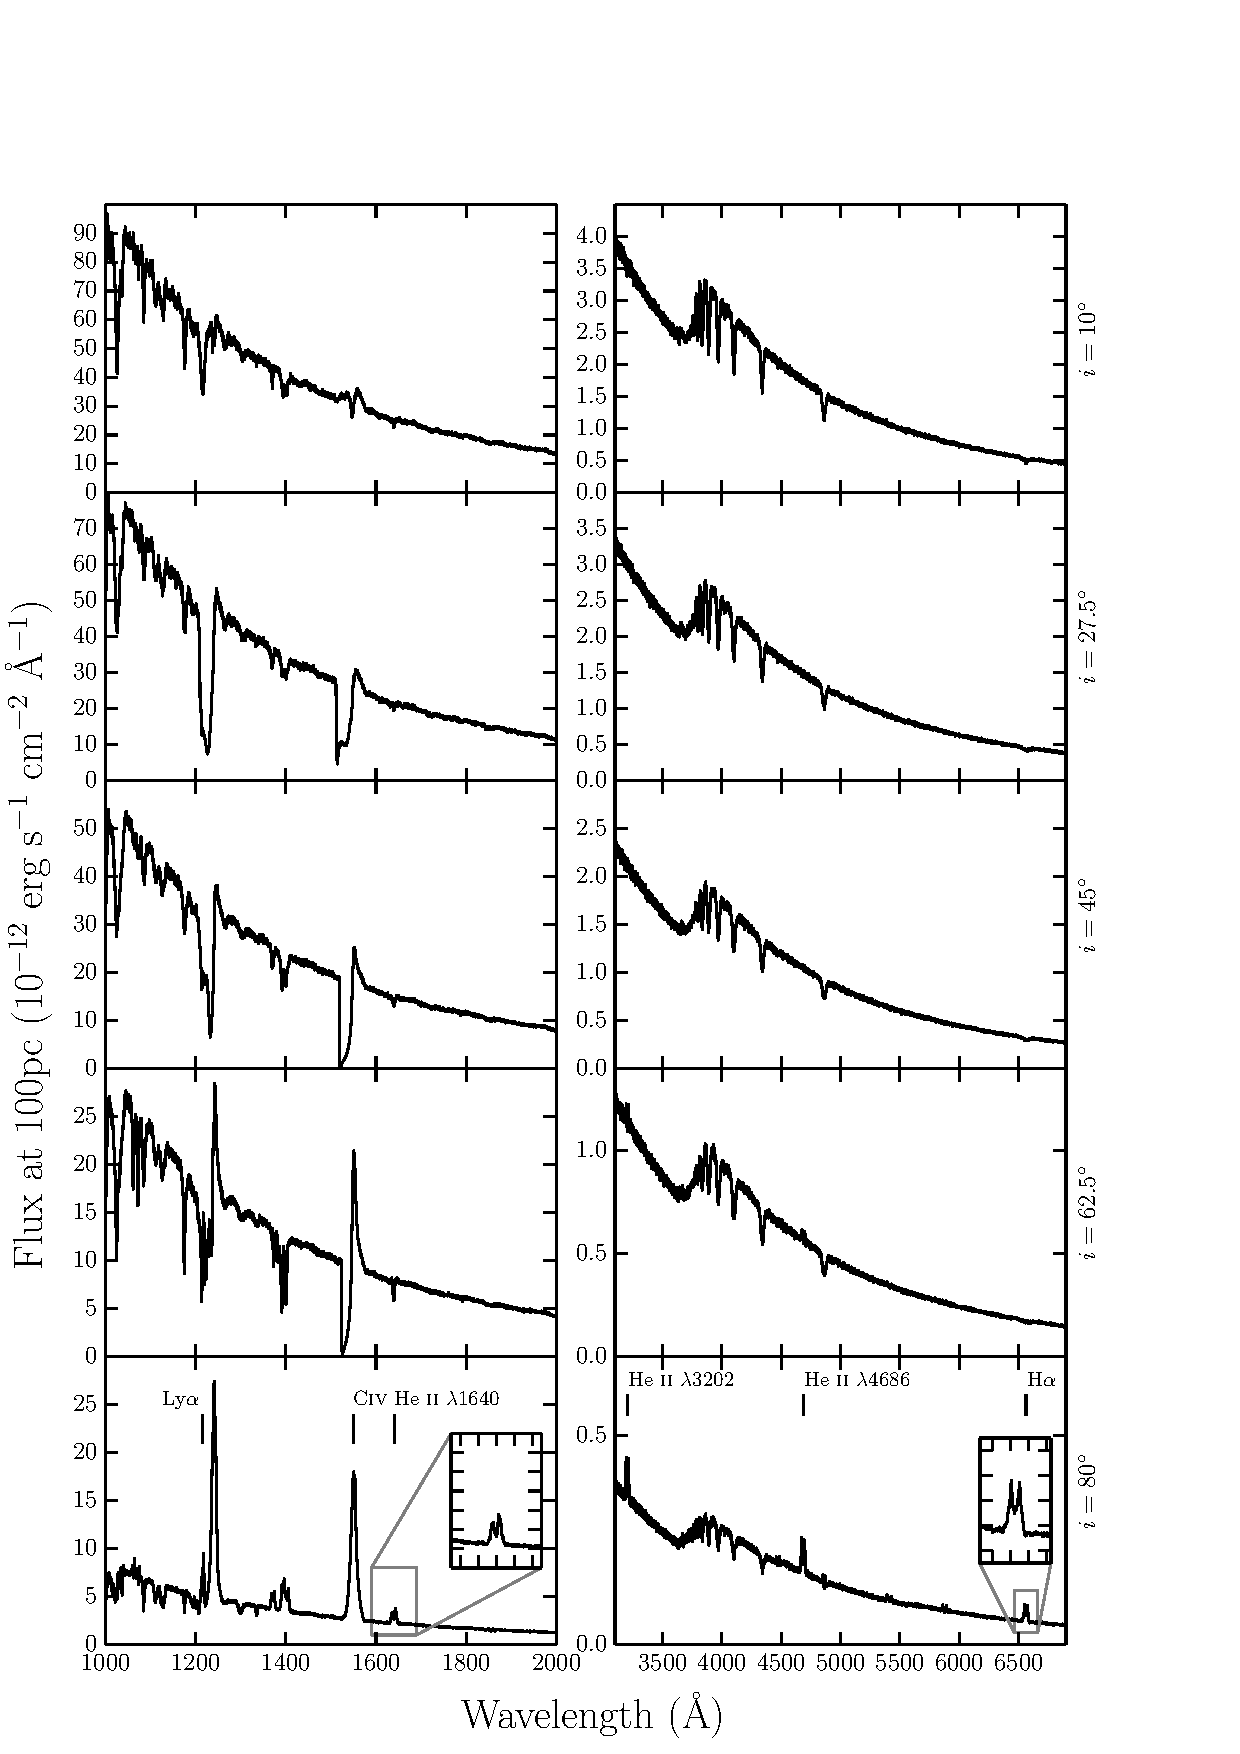
\includegraphics[width=1.0\textwidth]{figures/05-cvpaper/modela_uv_opt.png}
\caption
[UV and optical synthetic spectra from the benchmark CV model]{
UV (left) and optical (right) synthetic spectra for model A, the benchmark model,
computed at sightlines of 10, 27.5, 45, 62.5 and 80 degrees.	
The inset plots show zoomed-in line profiles for 
\heiiuv\ and \ha. Double-peaked line emission can be seen in 
\heiiuv, \heiiopt, \ha\ and some He I lines, but the 
line emission is not always sufficient to overcome the absorption
cores from the stellar atmosphere models. The model
also produces a prominent \heiioptnew\ line at high inclinations.
}
\label{spec}
\end{figure*}



\subsection{Synthetic Spectra}
\label{modela_spectrum}
\label{sec:modela_spectra}

I begin by verifying that the benchmark model still produces UV
spectra that resemble those observed in CVs. This should be
the case, since the ionization state of the wind has not changed
significantly from that computed by LK02 (see section~\ref{modela_ionization}). 
The left column of panels in Fig.~\ref{spec} shows that this expectation
is met: all of the strong metal resonance
lines -- notably N~\textsc{v}~$1240$~\AA,
Si~\textsc{iv}~$1400$~\AA\ and C~\textsc{iv}~$1550$~\AA\ -- 
are present and exhibit clear P-Cygni profiles
at intermediate inclinations. In addition, however, I now also find
that the wind produces significant Ly$\alpha$ and
He~\textsc{ii}~$1640$~\AA\ emission lines. 

Fig.~\ref{spec} (right-hand panel) and Fig.~\ref{spec_continuum}
show the corresponding optical spectra produced for
the benchmark model, and these do exhibit some emission lines
associated with H and He. There is 
a general trend from absorption lines to emission lines 
with increasing inclination, as we might expect from this wind
geometry. This trend is consistent with observations, as discussed in 
section~\ref{sec:NLs}. However, it is clear that this particular model
does not produce all of the lines seen in observations of high-state CVs.
The higher-order Balmer series lines are too weak
to overcome the intrinsic absorption from the disc atmosphere, and the wind 
fails to produce any observable emission at low and intermediate inclinations.
This contrasts with the fact that emission lines are seen 
in the optical spectra of (for example) V3885 Sgr \citep{hartley2005}
and IX Vel \citep[][see also Fig.~\ref{fig:NL_spec}]{beuermann1990}.

The emissivity of these recombination 
features scales as density squared, meaning that they form almost entirely in the 
dense base of the wind, just above the accretion disc. Here, the
velocity field of the wind is still dominated by rotation, rather than
outflow, which accounts for the double-peaked shape of the lines. In
principle, lines formed in this region can still be single peaked,
since the existence of a poloidal velocity {\em gradient} changes the
local escape probabilities (MC96). However, as
discussed further in section~\ref{sec:cv_line_shapes}, the 
radial velocity shear in the
models is not high enough for this radiative transfer effect
to dominate the line shapes.

The Balmer jump is in absorption at all inclinations for the benchmark
model. This is due to the stellar atmospheres used to
model the disc spectrum; it is not a result of photoabsorption in the
wind. In fact, the wind spectrum exhibits the Balmer jump in {\em
emission}, but this is not strong enough to overcome the intrinsic
absorption edge in the disc spectrum. This is illustrated in
Fig.~\ref{cont}, which shows the angle-integrated spectrum of the system,
i.e. the spectrum formed by all escaping photons, separated into the
disc and wind contributions. Even though the wind-formed Balmer
recombination continuum does not completely fill in the Balmer
absorption edge in this model, it does already contribute
significantly to the total spectrum. This suggests that modest changes 
to the outflow kinematics might boost the wind continuum and produce
emergent spectra with weak or absent Balmer absorption edges. 

\begin{figure}
\centering 
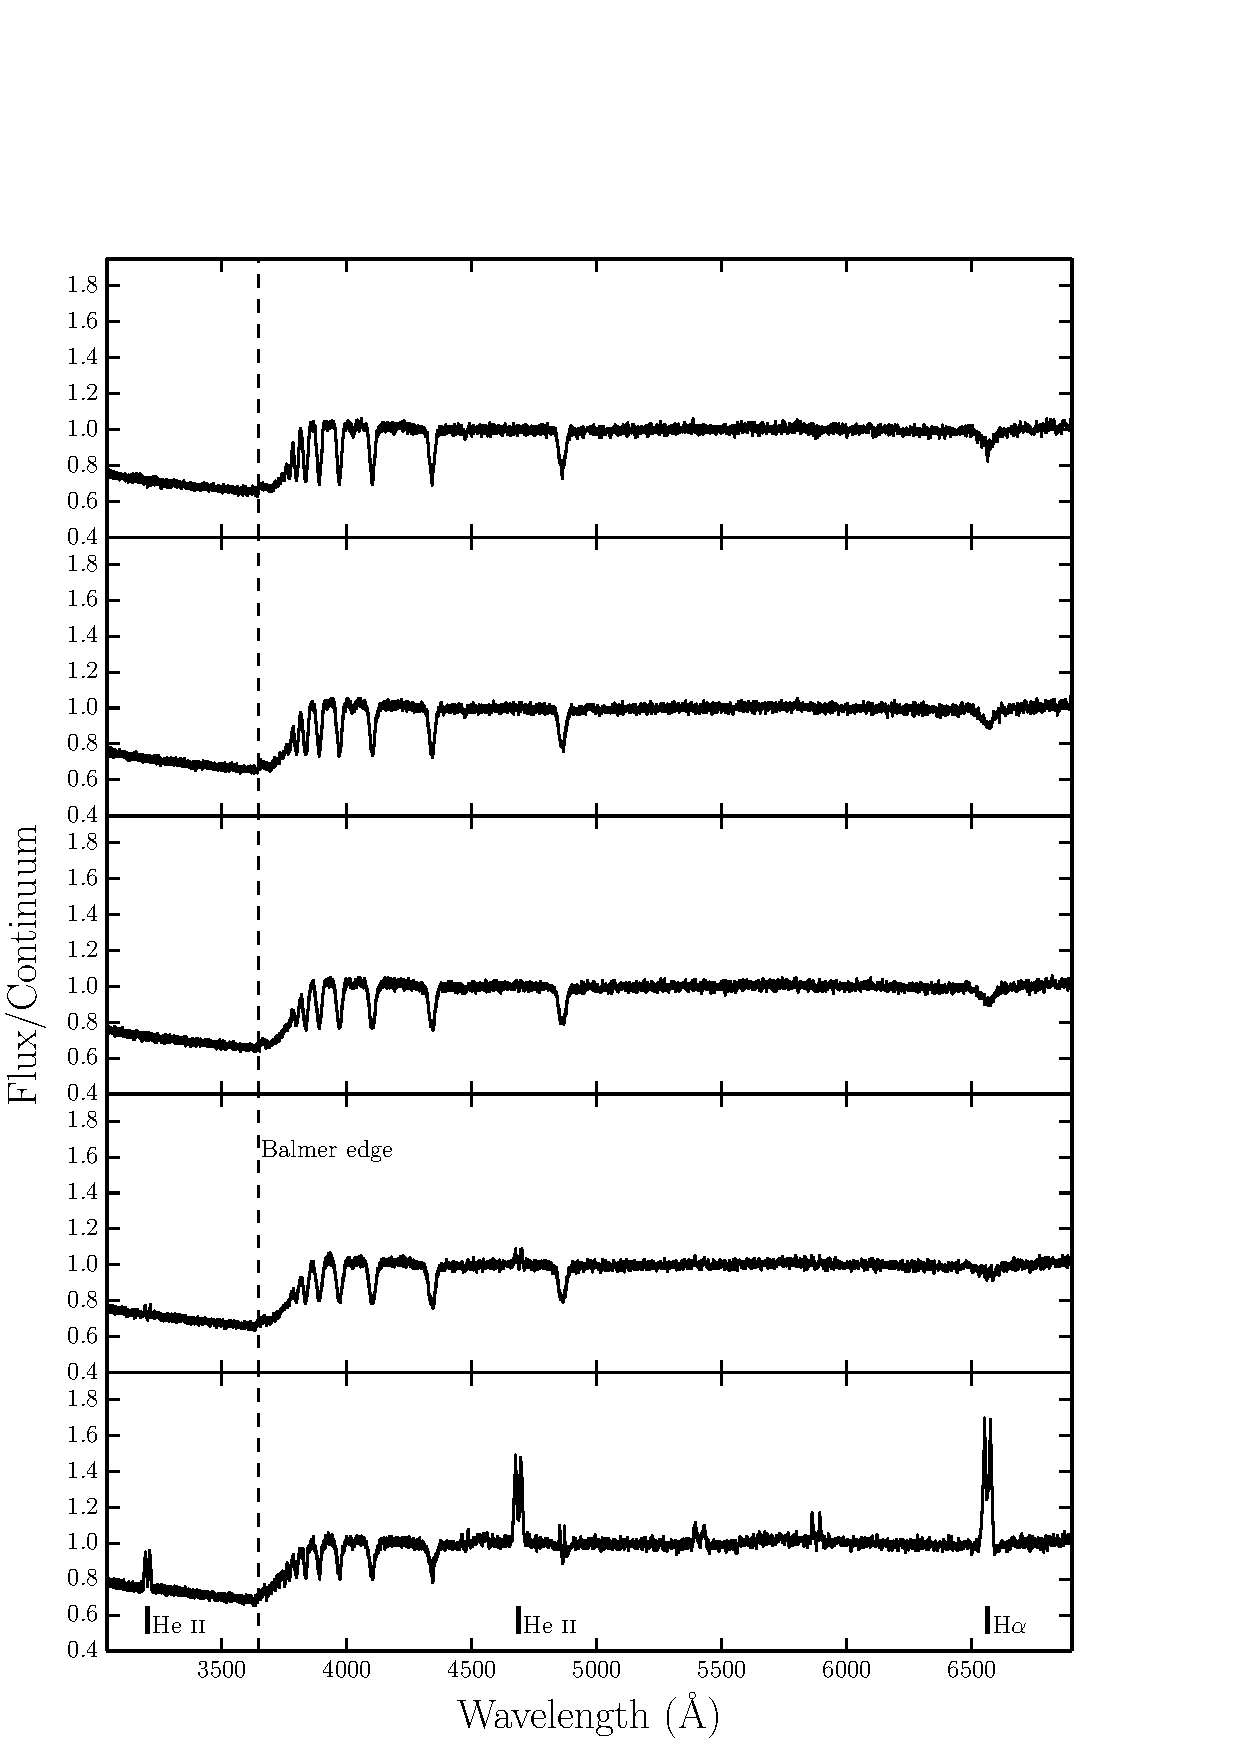
\includegraphics[width=1.0\textwidth]{figures/05-cvpaper/modela_opt_cont.png}
\caption
[Optical synthetic spectra from the benchmark CV model divided by the continuum.]
{Synthetic optical spectra from model A computed for 
sightlines of 10, 27.5, 45, 62.5 and 80 degrees. In these plots
the flux is divided by a polynomial fit to the 
underlying continuum redward of the Balmer edge, so that 
line-to-continuum ratios and the true depth of the
Balmer jump can be shown.}
\label{spec_continuum}
\end{figure} 

\begin{figure} 
\centering
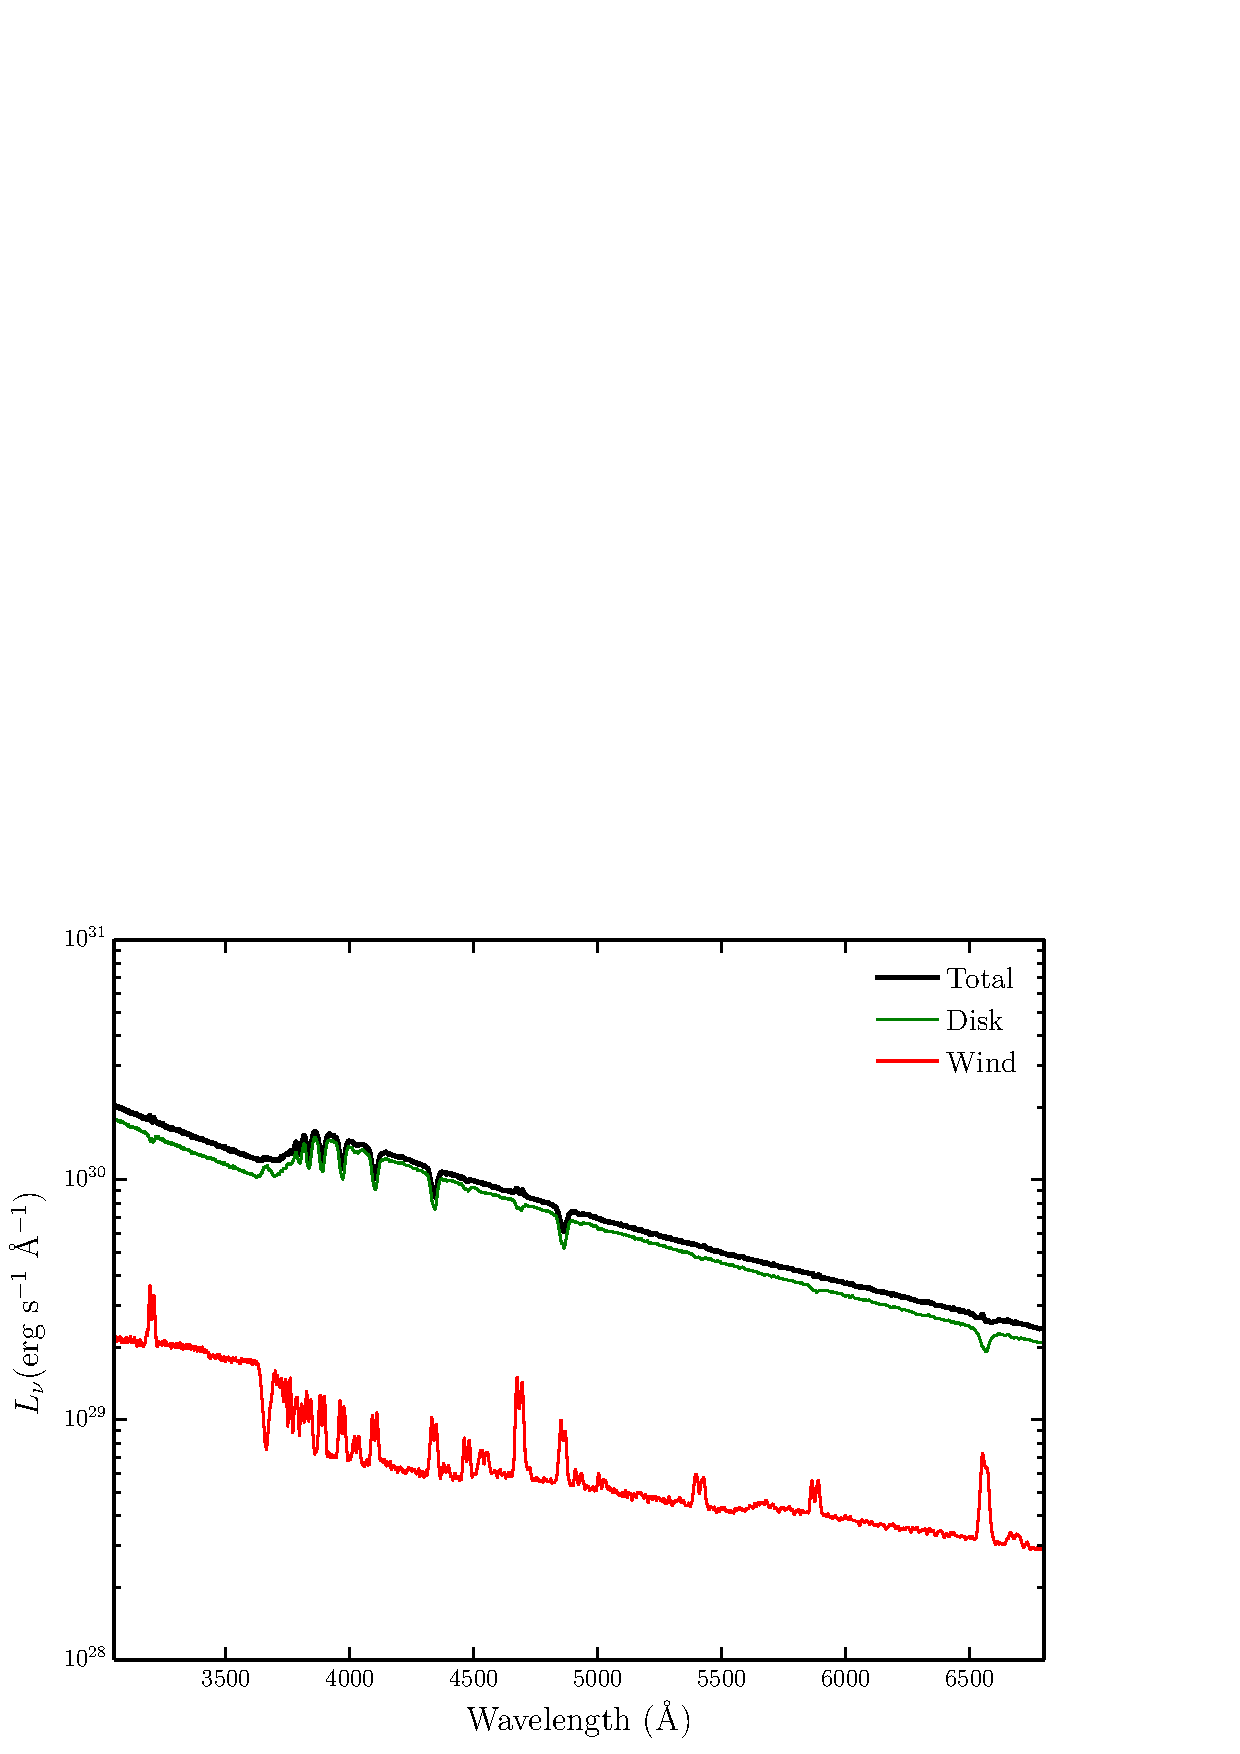
\includegraphics[width=1.0\textwidth]{figures/05-cvpaper/modela_escaping.png}
\caption
[Total packet-binned spectra across all viewing angles from the benchmark CV model.]
{Total packet-binned spectra across all viewing angles, in units
of monochromatic luminosity.
The thick black line shows the total 
integrated escaping spectrum, 
while the green line shows disc photons which escape without being reprocessed by
the wind. The red line show the contributions from reprocessed photons. 
Recombination continuum emission blueward of the Balmer 
edge is already prominent relative to other wind continuum processes, but is not sufficient
to fill in the Balmer jump in this specific model.}
\label{cont}
\end{figure} 


%\newpage



%%%%%%%%%%%%%%%%%%%%%%%%%%%%%%%%%%%%%%
%
%          REVISED MODEL
%
%%%%%%%%%%%%%%%%%%%%%%%%%%%%%%%%%%%%%%%

\section{A Revised Model Optimized for Optical Wavelengths}
\label{sec:modelb}
The benchmark model discussed in section~\ref{modela} was originally
designed to reproduce the wind-formed lines seen in the UV spectra of
high-state CVs. This model does produce some observable
optical emission, but I can now attempt to construct a model that more closely 
matches the observed optical spectra of CVs. 

Specifically, I aim to assess whether a revised model can:

\begin{itemize}
         \item account for all of the lines seen in optical spectra 
         of CVs while preserving
the UV behaviour;
         \item produce single-peaked Balmer emission lines; 
         \item generate enough of a wind-formed recombination continuum
to completely fill in the disc's Balmer absorption edge for 
reasonable outflow parameters.
\end{itemize} 

The emission measure of a plasma is directly proportional to its density.
The simplest way to simultaneously affect the density in the wind (for fixed mass-loss rate),
as well as the velocity gradients, is by modifying the poloidal velocity
law. Therefore, I focus on just two kinematic variables:

\begin{itemize}
         \item the acceleration length, $R_v$, which controls the
        distance over which the wind accelerates to $\frac{1}{2}~v_{\infty}$;
         \item the acceleration exponent, $\alpha$, which controls the rate 
         at which the poloidal velocity changes near $R_v$.
\end{itemize} 

The general behaviour we might expect is that outflows with denser
regions near the wind base -- i.e. winds with larger $R_{v}$ and/or
larger $\alpha$ -- will produce stronger optical emission signatures. 
However, this behaviour may be moderated by the effect of the increasing
optical depth through this region, which can also affect the line profile shapes. 
In addition, modifying $R_v$ also increases the emission {\em volume}.
Based on a preliminary exploration of models with different kinematics,
I adopt the parameters listed in table~\ref{modelb_table}
for this new, `optically optimized' model (model B). 

%It is possible that other parameters, such as the launching radii and angles



\subsection{Synthetic Spectra}
\label{sec:modelb_spectra}
\begin{figure*}
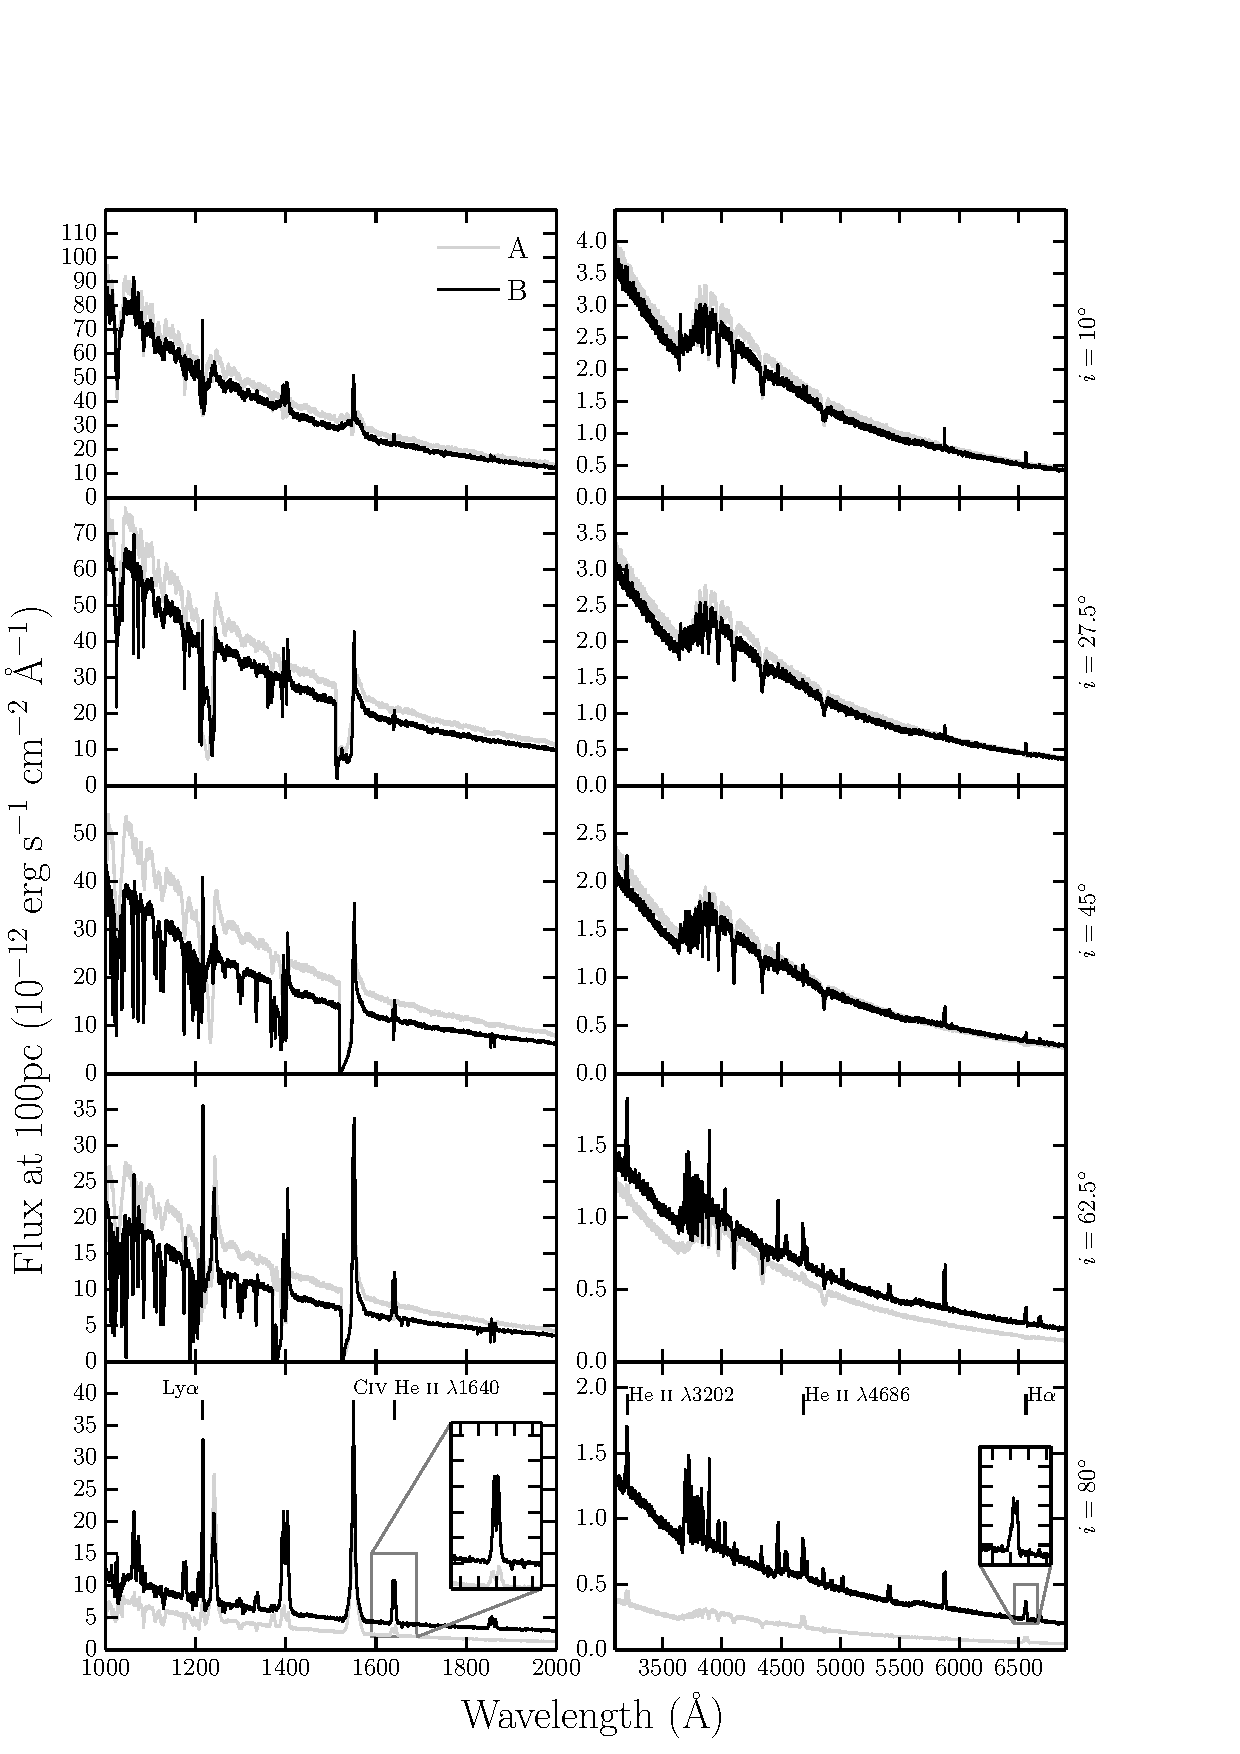
\includegraphics[width=1.0\textwidth]{figures/05-cvpaper/modelb_uv_opt.png}
\caption
[UV and optical synthetic spectra from CV model B]{
UV (left) and optical (right) synthetic spectra for model B computed at
sightlines of 10, 27.5, 45, 62.5 and 80 degrees. 
Model A is shown in grey for comparison.	
The inset plots show zoomed-in line profiles for 
\heiiuv\ and \ha. The Balmer and He
are double-peaked, albeit with narrower profiles.
Strong \heiiopt\ emission can be seen, as well as a trend
of a deeper Balmer jump with decreasing inclination.
}
\label{uvoptb}
\end{figure*}

Fig.~\ref{uvoptb} shows the UV and optical spectra for the
optically optimized model for the full range of inclinations. 
As expected, the trend from absorption to emission 
in the optical is again present, but in this revised model emission
lines in the entire Balmer series are produced at high inclinations, as well
as the observed lines 
in He~\textsc{ii} and He~\textsc{i}. This can be seen more clearly in the 
continuum-normalized spectrum in Fig.~\ref{continuumb}.

Two other features are worth noting in the optical
spectrum. First, the collisionally excited Ca~{\sc ii} emission line at $3934$~\AA\ 
becomes quite prominent in the densest models. Second, the model predicts a detectable
He~\textsc{ii} recombination line at $3202$~\AA. This is the He
equivalent of Paschen~$\beta$ and should be expected in all systems that
feature a strong He~\textsc{ii}~$4686$~\AA\ line (the He
equivalent of Paschen~$\alpha$). 
This line is somewhat unfamiliar observationally, because it 
lies bluewards of the atmospheric cut-off, but
also redwards of most ultraviolet spectra. 

The synthetic spectra do not exhibit P-Cygni profiles in the optical lines.
This is perhaps not surprising. LK02 and SV93 originally designed such models
to reproduce the UV line profiles. Thus, most of the wind
has an ionization parameter of $\log U \sim 2$ (see Fig.~\ref{wind}).
This means H and He are mostly ionized throughout 
much of the wind and are successful in producing recombination features.
However, the line opacity throughout the wind is too
low to produce noticeable blue shifted absorption in these lines. 
It appears that the systems that exhibit such profiles must 
possess a higher degree of ionization stratification, although the lack 
of contemporary observations means it is not known for certain if the 
P-Cygni profiles in UV resonance lines and optical H and He lines exist simultaneously.
Ionization stratification could be caused by a clumpy flow, in which the 
ionization state 
changes due to small scale density fluctuations, or a stratification in density
and ionizing radiation field over larger scales.
Invoking clumpiness in these outflows is not an unreasonable
hypothesis. Theories of line-driven winds predict an unstable flow
\citep{macgregor1979,owockirybicki1984,owockirybicki1985}, and
simulations of CV disc winds also produce density inhomogeneities 
\citep{proga1998,pkdh2002}.
Tentative evidence for clumping being directly related to P-Cygni optical lines
comes from the fact that \cite{prinja2000}
found the dwarf nova BZ Cam's outflow to be unsteady and highly mass-loaded in outburst,
based on observations of the UV resonance lines.
This system has also exhibited P-Cygni profiles in He~\textsc{i}~$5876$~\AA
and \ha\ when in a high-state \citep{patterson1996,RN98}. 
The degree of ionization and density variation and 
subsequent line opacities may be affected by the model parameters
and the specific parameterisation adopted.

In the UV, the model still produces all the observed lines, 
and deep P-Cygni profiles are produced in the normal resonance lines,
as discussed in section~\ref{sec:modela_spectra}. However, the UV spectra also
display what is perhaps the biggest problem with this revised model,
namely the strength of resonance line emission 
at low and intermediate inclinations.
In order to generate strong optical wind signatures, I have adopted wind
parameters that lead to very high densities at the base of the wind
($n_e\sim10^{13}-10^{14}$~cm$^{-3}$). This produces
the desired optical recombination emission, but also increases the
role of collisional excitation in the formation of the UV resonance
lines. This explains the pronounced increase in the emission component 
of the C\textsc{iv} $1550$~\AA\ resonance line, for example, relative to
what was seen in the benchmark model (compare Figures~\ref{spec} and
\ref{uvoptb}). The strength of this component in the revised model 
is probably somewhat too high to be consistent with UV observations 
of high-state CVs \citep[see e.g.][]{long1991,long1994, noebauer}.


\subsection{Continuum Shape and the Balmer Jump}

The wind now also has a clear effect on the continuum shape,
as shown by Fig.~\ref{modelb_escape}. In fact, the majority of the
escaping spectrum has been reprocessed in some way by the wind,
either by electron scattering (the wind is now moderately Thomson-thick),
or by bound-free processes. This is demonstrated by the flatter spectral shape
and the slight He photoabsorption edge present in the optical spectrum 
(marked in Fig.~\ref{continuumb}). This reprocessing is also
responsible for the change in continuum level between models A and B.
In addition, Figures~\ref{uvoptb}, \ref{continuumb} 
and \ref{modelb_escape} clearly demonstrate that the wind produces
a recombination continuum sufficient to completely fill in the Balmer jump
at high inclinations.\footnote{Note that the apparent absorption feature 
just redward of the Balmer jump in these models is artificial. It is
caused by residual line blanketing in the stellar atmospheres, which
the models cannot fill in since they employ a 20-level H atom.}
This might suggest that Balmer continuum emission from a wind can be important 
in shaping the Balmer jump region, as
suggested by \cite{KLWB98} and \cite{hassall}.

It should be acknowledged, however,
that the Balmer jump in high-state CVs would naturally weaken at
high inclinations due to limb darkening effects \citep{ladous1989, ladous1989b}. 
Although simple limb darkening law which affects 
the emergent flux at each inclination is included,
it is not a {\em frequency dependent} opacity in the model.
As a result, the efficiency of filling in the Balmer jump
should really be judged at low and medium inclinations, 
where, although prominent, the recombination continuum does
not overcome the disc atmosphere absorption. 
In addition, this effect 
could mean that any model which successfully fills in the 
jump at low inclinations could lead to a Balmer jump 
in emission at high inclinations.
Furthermore, in this particular model,
approximately $10\%$ of the overall luminosity ultimately
hits the surface of one of the photon sources and is destroyed.
Neglecting, this backscattered radiation could have a small effect on the temperature
and ionization structure of the disc and lower wind region. Irradiation of the disc
by the WD is insignificant, as the high accretion rate causes the disc 
to dominate the emergent luminosity (see e.g. Fig.~\ref{cv_model_sed}).
In any case, to properly understand the 
effect of inclination and irradiation on the resultant 
Balmer jump, a fully self-consistent
radiative transfer calculation of both the disc atmosphere
and connected wind is required. 

\begin{figure} 
\centering
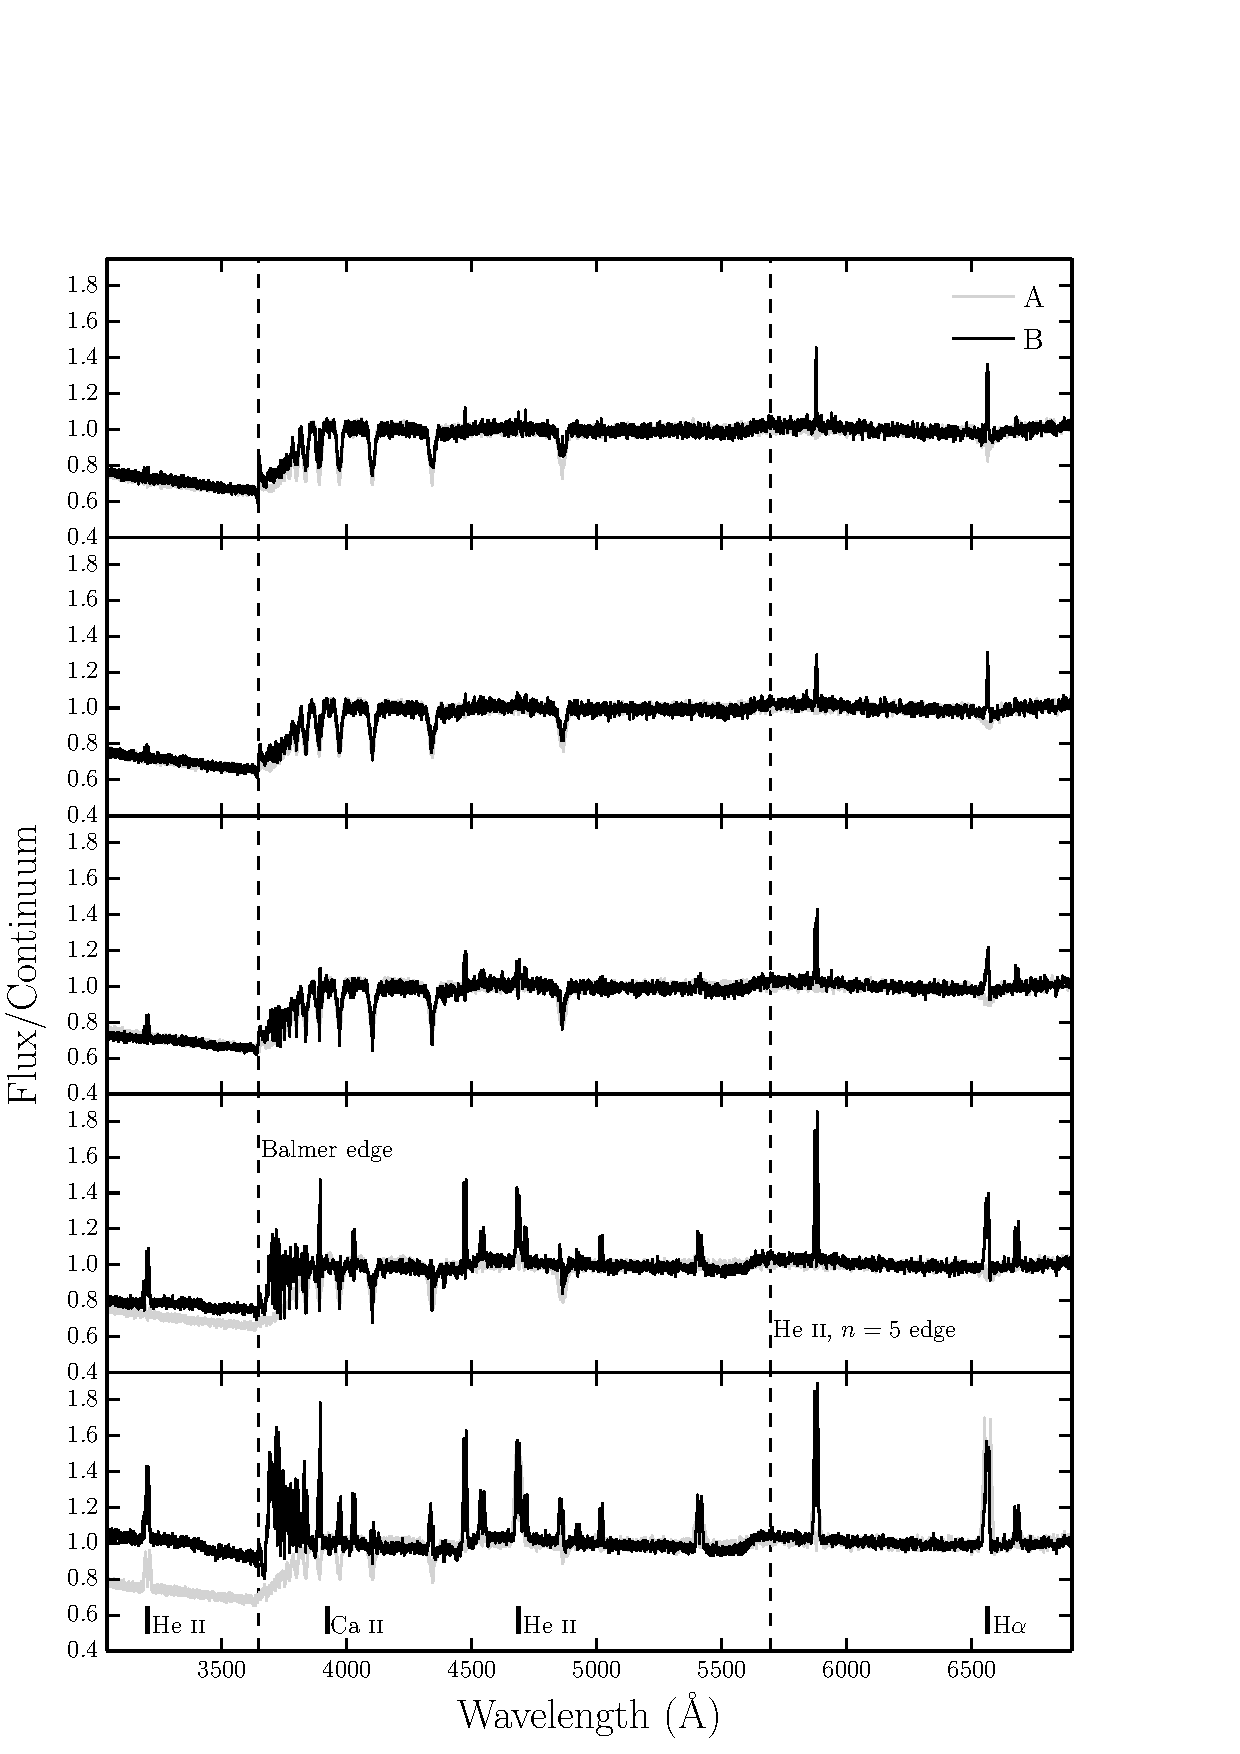
\includegraphics[width=1.0\textwidth]{figures/05-cvpaper/modelb_opt_cont.png}
\caption
[Optical synthetic spectra from CV model B divided by the continuum.]{
Synthetic optical spectra from model B computed for 
sightlines of 10, 27.5, 45, 62.5 and 80 degrees. 
Model A is shown in grey for comparison.
In these plots the flux is divided by a polynomial fit to the 
underlying continuum redward of the Balmer edge, so that 
line-to-continuum ratios and the true depth of the
Balmer jump can be shown.
}
\label{continuumb}
\end{figure} 

\begin{figure} 
\centering
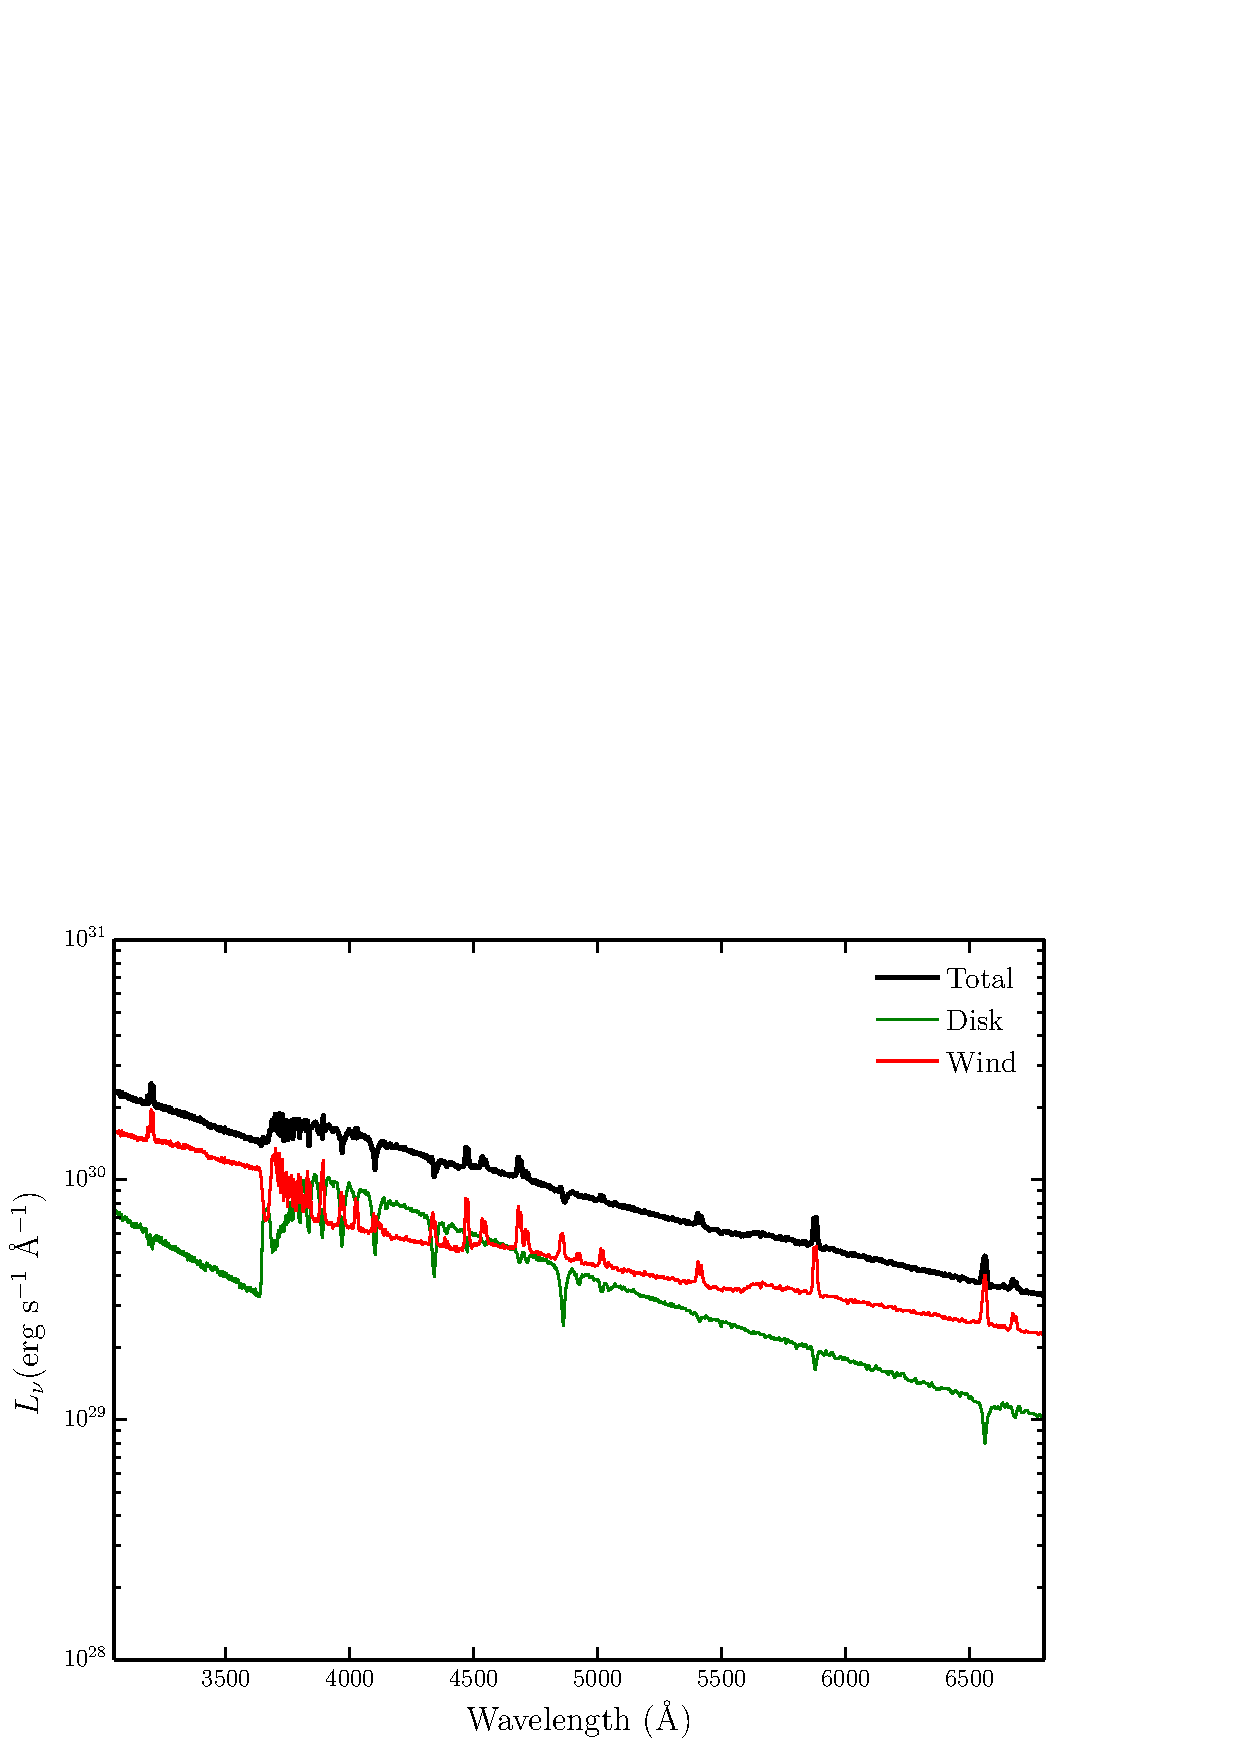
\includegraphics[width=1.0\textwidth]{figures/05-cvpaper/modelb_escaping.png}
\caption
[Total packet-binned spectra across all viewing angles from CV model B.]
{Total packet-binned spectra across all viewing angles, in units
of monochromatic luminosity. 
The thick black line shows the total 
integrated escaping spectrum, 
while the green line shows disc photons which escape without being reprocessed by
the wind. The red line show the contributions from reprocessed 
photons. 
In this denser model the reprocessed contribution is significant compared
to the escaping disc spectrum. The Balmer continuum emission is prominent, and
the wind has a clear effect on the overall spectral shape.}
\label{modelb_escape}
\end{figure} 

\begin{figure}
\centering
\includegraphics[width=1.0\textwidth]{figures/05-cvpaper/mc.png}
\caption
[\ha\ line profiles from CV models A, B and X]
{
\ha\ line profiles, normalized to 1, plotted in velocity space 
for three models with varying kinematic 
properties, computed at an inclination of $80^\circ$.
The benchmark model and the improved optical
model described in section~\ref{sec:modelb} are labeled as A and B respectively,
and a third model (X) which has an increased acceleration length of 
$R_v = 283.8~R_{WD}$, and $\alpha=4$ is also shown. 
The $x$-axis limits correspond to the Keplerian velocity at 
$4~R_{WD}$, the inner edge of the wind.
There is a narrowing of the lines, and a single-peaked line in model X.
This is not due to radial velocity shear (see section~\ref{sec:cv_line_shapes}).
}
\label{halpha}
\end{figure} %fullpage






\subsection{Line Profile Shapes: Producing Single-Peaked Emission}
\label{sec:cv_line_shapes}

Fig.~\ref{halpha} shows how the H$\alpha$ profile changes with the kinematics of the wind for 
an inclination of $80^\circ$. The main prediction is that dense, slowly accelerating 
wind models produce narrower emission lines. This is {\em not} due to radial 
velocity shear. As stated by MC96, that mechanism can only work if poloidal 
and rotational velocity gradients satisfy $(dv_l/dr)/(dv_\phi/dr) \gtrsim 1$; in 
these models, this ratio is always $\lesssim 0.1$. Instead, the narrow lines predicted 
by the denser wind models can be traced to the base of the outflow becoming optically 
thick in the continuum, such that the line emission from the base of the wind
cannot escape to the observer. In such models, the `line photosphere'
(the $\tau \simeq 1$ surface of the line-forming region) moves outwards, towards larger 
vertical and cylindrical distances. This reduces the predicted line widths, since the 
rotational velocities -- which normally provide the main line broadening mechanism at 
high inclination -- drop off as $1/r$ in the outflow. This $1/r$ behaviour occurs due to the wind
conserving specific angular momentum, and is initially in Keplerian rotation 
(see equation~\ref{eq:vrot}). The fact that the MC96 
mechanism does not significantly affect the line profiles in this specific model 
does not mean that it could not be at work in CV winds. For example, it would be worth investigating
alternative prescriptions for the wind velocity field, as well as the possibility that the 
outflows may be clumped. An inhomogeneous flow 
(which has been predicted in CVs; see section~\ref{sec:modelb_spectra})
might allow large radial velocity shears to exist while still 
maintaining the high densities needed to produce the required level of emission.
However, such an investigation is beyond the scope of the present study.

In these models, single-peaked line profiles are produced once the line forming region 
has been
pushed up to $\sim 10^{11}$~cm ($\sim150~R_{WD}$) above the disc plane. 
This number may seem unrealistically large, but the vertical extent of 
the emission region is actually not well constrained observationally. 
In fact, multiple observations of eclipsing NLs show that the H$\alpha$ 
line is only moderately eclipsed compared to the continuum 
\citep[e.g.][see also section~\ref{sec:rwtri}]{baptista2000,groot2004}, 
implying a significant vertical extent for the line-forming 
region. This type of model should therefore not be ruled out {\em a priori}, 
but this specific model was not adopted as the optically optimized model
due to its unrealistically high continuum level in eclipse. 

Observations could help to assess the viability of this scenario, in which lines 
are single peaked due to being formed high above the disc plane. The line formation
region is roughly cospatial with the main recombination continuum emission region.
Thus, the in and out of eclipse continuum levels of high-inclination CVs should be 
compared to see how much of any extended wind emission is occulted by the 
donor star, allowing limits to be placed on
the emission region size. Directly imaging the continuum emission region may prove harder.
At a typical NL distance of $200$~pc \citep[e.g.][]{knigge2006,mizusawa2010}, 
the angular size of a region of size $10^{11}$~cm is approximately $5$~mas. This lies beyond the 
capabilities of the {\sl Hubble Space Telescope}\footnote{http://www.spacetelescope.org/about/general/instruments/wfc3/} and the future {\sl James Webb Space Telescope}
\footnote{http://jwst.nasa.gov/facts.html}.
If the emission region is more extended, on the order of $10^{12}$~cm, resolving it may just 
be possible in the case of the closest NLs and high-state 
DNe \citep[at $\sim100$~pc, e.g.][]{millerjones2013}, which would represent 
the first direct observation of a disc wind. Generally, however, this specific
observation appears to be challenging for even the next generation of 
space telescopes.



%\footnote{https://almascience.eso.org/alma-science}


\subsection{Sensitivity to Model Parameters}
\label{sec:cv_params}
This revised model demonstrates that one can achieve a more
realistic optical spectrum by altering just two kinematic parameters. 
However, it may also be possible to achieve this by modifying
other free parameters such as $\dot{M}_{W}$, the opening angles of the wind and the 
inner and outer launch radii. For example, increasing the mass-loss rate of the wind
increases the amount of recombination emission (which scales with density squared), 
as well as lowering the ionization parameter and increasing the optical depth through the wind. 
Larger launching regions and covering factors tend to lead to a larger emitting volume, 
but this is moderated by a decrease in density 
for a fixed mass-loss rate. I also note that the inner radius of $4~R_{WD}$ adopted by SV93 
affects the emergent UV spectrum seen at inclinations $<\theta_{\mathrm{min}}$ as 
the inner disc is uncovered. This causes less absorption in the UV resonance lines,
but the effect on the optical spectrum is negligible.
I have verified this general behaviour, but
I suggest that future work should investigate the effect of these parameters in more detail,
as well as incorporating a treatment of clumping.
If a wind really does produce the line and continuum emission seen in optical spectra of high-state CVs, then
understanding the true mass-loss rate and geometry of the outflow is clearly important.


\subsection{Comparison to RW Tri}
\label{sec:rwtri}
\begin{figure*}
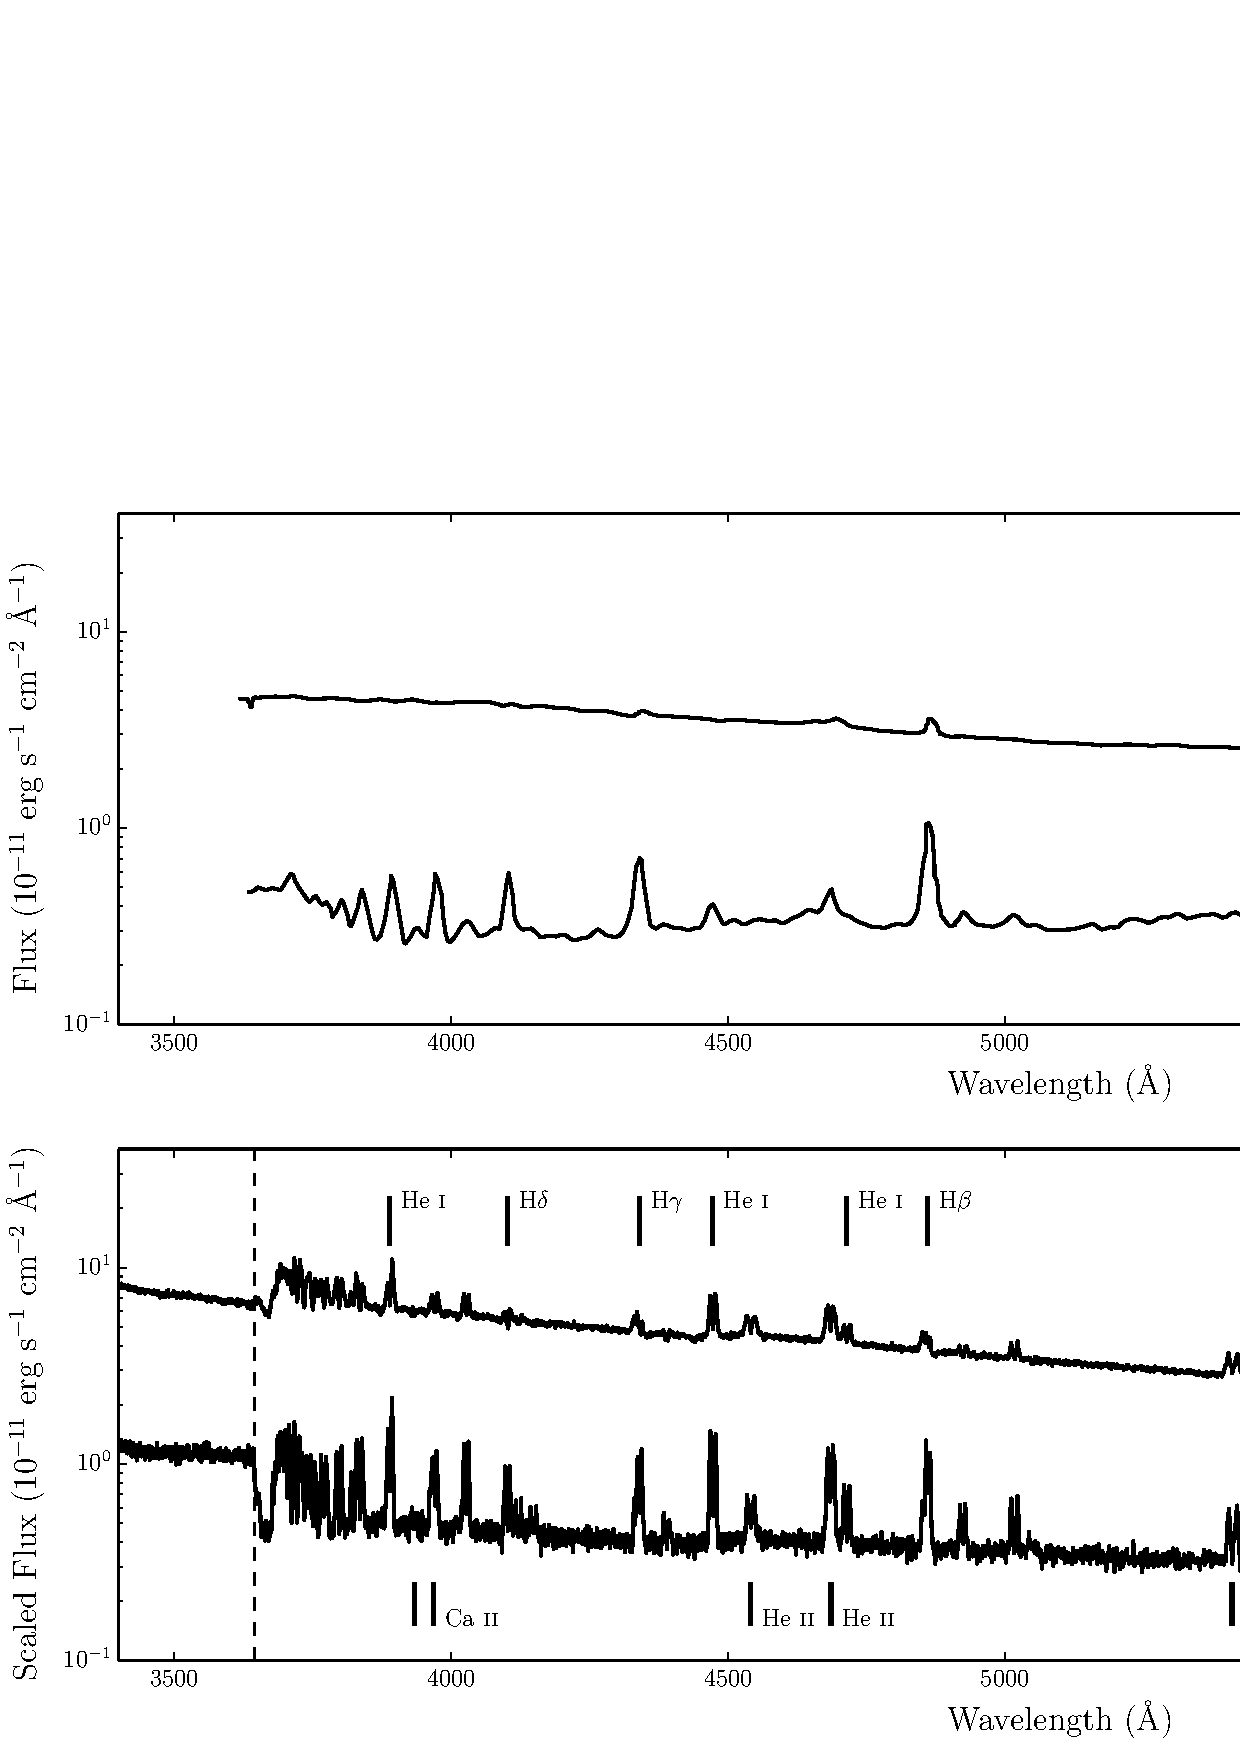
\includegraphics[width=0.9\textheight, angle=270]{figures/05-cvpaper/fig13.png}
\caption
[In and out of eclipse spectra from model B compared to the high
inclination NL RW Tri]
{{\sl Top Panel:} In and out of eclipse spectra of the high
inclination NL RW Tri. {\sl Bottom Panel:} In and out of eclipse synthetic
spectra from model B.
The artificial `absorption' feature just redward of the Balmer jump
is due to the reasons described in section 5.2.}
\label{rwtricomp}
\end{figure*}

Fig.~\ref{rwtricomp} shows a comparison of the predicted
out-of-eclipse and mid-eclipse spectra against observations of the
high-inclination nova-like RW~Tri. The inclination of RW Tri is
somewhat uncertain, with estimates including $70.5^\circ$
\citep{smak1995}, $75^\circ$ \citep{groot2004}, $80^\circ$
\citep{longmore1981} and $82^\circ$\citep{frankking1981}. Here, we
adopt $i = 80^\circ$, but the qualitative conclusions are not
particularly sensitive to this choice. 
I follow LK02 is setting the value of $r_{\mathrm{disc}}(\mathrm{max})$ (the maximum radius of the accretion disc)
to $34.3~R_{WD}$. When compared to the semi-major axis of RW Tri,
this value is perhaps lower than one might 
typically expect for NLs \citep{harropallinwarner1996}. 
However, it is consistent
with values inferred by \cite{rutten1992}.
I emphasize that this model is in no sense a fit to this -- or any other -- data set.


The similarity between the synthetic and observed spectra is
striking. In particular, the revised model produces strong emission in
all the Balmer lines, with line-to-continuum ratios comparable to
those seen in RW Tri. Moreover, the line-to-continuum contrast
increases during eclipse, as expected for emission produced in a disc
wind. This trend is in line with the observations of RW~Tri, and it
has also been seen in other NLs, including members of the SW~Sex class
\citep{neustroev2011}. As noted in section~\ref{sec:modelb_spectra}, the majority
of the escaping radiation has been reprocessed by the wind in some way
(particularly the eclipsed light).

However, there are also interesting differences between the revised
model and the RW Tri data set. For example, the synthetic spectra exhibit
considerably stronger He~{\sc ii} features than the observations,
which suggests that the overall ionization state of the model is
somewhat too high. As discussed in section~\ref{sec:cv_line_shapes}, 
the optical lines are narrow, but double-peaked. 
This is in contrast to what is generally seen in observations
of NLs, although the relatively low resolution of the RW Tri
spectrum makes a specific comparison difficult. In order to demonstrate
the double-peaked nature of the narrower lines, I do not 
smooth the synthesized data to the resolution of the RW Tri dataset.
If the data was smoothed, the \ha\ line would appear single-peaked.

\subsection{A Note on Collision Strengths}
\label{sec:coll_bl}

\py\ uses the \cite{vanregemorter} approximation 
(see section~\ref{sec:coll}) to calculate collision rates.
This approach uses an effective gaunt factor, $\bar{g}$, of
order unity. To conduct these specific simulations a value of $\bar{g}=1$ 
was adopted. There are two main concerns when using this approach.
The first is related to accuracy, as poorly estimating collision strengths
could lead to incorrect heating and cooling balance in the flow, with
knock-on effects on the emergent spectrum. This is of particular concern
here as line heating is the dominant heating mechanism in the dense 
base of the wind. I have verified that the main conclusions of this study
are fairly insensitive to the gaunt factor; for example, if I adopt
$\bar{g}=0.2$ as suggested by, e.g., \cite{ferland2005} than the wind still
produces a host of recombination lines. 
If improved collision strengths were to significantly reduce the wind temperature
a boundary layer might
actually be required to produce the higher ionization lines such as 
\heiiopt\ \citep[see e.g.][]{hoare1991}, arguably making the model
more realistic.

The second concern is that 
collisions between radiatively forbidden transitions are not taken into 
account when one splits levels into $l$- and $s$-subshells, as well
as principal quantum number, $n$ (as I have done with He~\textsc{i}; 
see section~\ref{sec:atomic_data}). However, I have verified that
in this case the plasma is dense enough, and ionized enough, 
that recombination dominates the level populations, at least in 
the regions responsible for the optical line emission. In other words, two levels
that are linked only by a forbidden transition have their relative populations
determined by their recombination rates from the upper ion.
Nevertheless, for future efforts, it would be desirable to include
collisional data for forbidden transitions, an effort that has now
been started (see chapter 7).



% \subsection{Model Sensitivity to Collision Strengths}
% \subsubsection{Collisions Between Radiatively Forbidden Transitions}
% \label{sec:rad_forbid}
% \subsubsection{Line Heating and Cooling}
% \label{sec:line_heat}
% Fig.~?? shows four important heating and cooling mechanisms 
% in the wind for model B. Line heating and cooling 
% \subsection{Improving Collision Strengths}
% \subsection{Introducing a Boundary Layer}



%%%%%%%%%%%%%%%%%%%%%%%%%%%%%%%%%%%%%%
%
%          CONCLUSIONS
%
%%%%%%%%%%%%%%%%%%%%%%%%%%%%%%%%%%%%%%%


\section{Conclusions}
\label{sec:cv_conclusions}

I have investigated whether a disc wind model designed to reproduce
the UV spectra of high-state CVs would also have a significant effect
on the optical spectra of these systems. I find that this is indeed
the case. In particular, the model wind produces H and He
recombination lines, as well as a recombination continuum blueward of
the Balmer edge. The spectra do not show P-Cygni profiles
in the optical H and He lines, which are seen in a small fraction of CV 
optical spectra. Possible reasons for this are briefly discussed in 
section~\ref{sec:modelb_spectra}.

A revised benchmark model was also constructed
to more closely match the optical spectra of high-state CVs. This
optically optimized model produces all the prominent optical lines in
and out of eclipse and achieves reasonable verisimilitude with the
observed optical spectra of RW Tri. However, this model also has
significant shortcomings. In particular, it predicts
stronger-than-observed He~{\sc ii} lines in the optical region and too
much of a collisionally excited contribution to the UV resonance lines. 
Incorporating more accurate collisional data into \py\ will help
assess this discrepancy in more detail.

Based on these results, I argue that recombination emission 
from outflows with sufficiently high densities and/or optical depths 
might produce the optical lines observed in CVs. It may also 
fill in the Balmer absorption edge in the spectrum of the accretion disc, 
thus accounting for the absence of a strong edge in observed CV spectra.
In section~\ref{sec:cv_line_shapes}, I demonstrated that
although the double peaked lines narrow and 
single-peaked emission can be formed in the densest models, 
this is not due to the radial velocity shear mechanism proposed by MC96.
I suggest that `clumpy' line-driven winds or a different
wind parameterization may nevertheless allow this mechanism to work.
I also note the possibility that, as seen in the densest models I have presented, 
the single-peaked lines are formed well above the disc, where 
rotational velocities are lower.

It is not yet clear whether a wind model such as this can
explain all of the observed optical features of high-state CVs --
further effort is required on both the observational
and modelling fronts. However, this work demonstrates that disc winds may
not just be responsible for creating the blue-shifted absorption and
P-Cygni profiles seen in the UV resonance lines of high-state CVs, but
can also have a strong effect on the optical appearance of these
systems. In fact, most of the optical features characteristic of CVs
are likely to be affected -- and possibly even dominated -- by their disc
winds. Given that optical spectroscopy plays a central role in
observational studies of CVs, it is critical to know 
where and how these spectra are actually formed. I believe it is high
time for a renewed effort to understand the formation of spectra in
accretion discs and associated outflows. 


  % Experiment 1

\newpage
\lhead{\emph{5. Testing Quasar Unification: Radiative Transfer In Clumpy Winds}}  
\chapter{Testing Quasar Unification: Radiative Transfer In Clumpy Winds}

{\em This chapter is based on the publication:

Matthews J. H., Knigge C., Long K. S., Sim S. A., Higginbottom N., Mangham S. W., 
`Testing quasar unification: radiative transfer in clumpy winds',
2016, MNRAS, 458, 293.}


%%%%%%%%%%%%%%%%%%%%%%%%%%%%%%%%%%%%%%
%
%          INTRODUCTION
%
%%%%%%%%%%%%%%%%%%%%%%%%%%%%%%%%%%%%%%%

\section{Introduction}

In chapters 1 and 2, I reviewed the observational evidence for accretion disc
winds in quasars and luminous AGN, and showed how they may be responsible
for more than just the broad absorption lines and P-Cygni profiles
seen in quasar spectra. In particular, they offer a natural way to
{\em unify} much of the complex phenomenology into one simple picture.

Here, I aim to test that picture using \py, with
the specific aim of determining whether it is possible to 
reproduce the key properties of AGN spectra, including those of BALQSOs, 
using simple kinematic prescriptions for biconical disc winds. 
Past results have been encouraging: H13
produced simulated spectra that resembled those of BALQSOs, as long as 
the luminosity of the X-ray source was relatively low, of order 
\POW{43}{\LUM}, and the mass-loss rate was relatively high, of order the 
mass accretion rate.  However, at higher X-ray luminosities, the wind was
so ionized that UV absorption lines were not produced.  In addition, and 
in part due to limitations inherent in 
the radiative transfer methods, the model failed 
to produce spectra with strong emission lines at any inclination angle.

Here I attempt to address both of these issues, by
allowing for clumping in the outflow and a introducing a more complete
treatment of H and He in the radiative transfer calculations.
Thus, the simulations presented in this chapter treat H and He as full
macro-atoms and metals as simple-atoms, as described extensively
in chapter 3. In order to correctly model the ionizing spectrum for simple-atoms,
I dispense with the dilute blackbody modified-Saha approach and fully solve the ionization
balance using the spectral modelling approach described 
in section~\ref{sec:simple_ionization}. Macro-atoms still have their
ionization and excitation states calculated from MC estimators.

The kinematic model used once again follows the SV93
prescription, and is described, together with the clumping 
implementation, in section~\ref{sec:clumpy_wind_model}.
Section~\ref{sec:qso_results} contains the results obtained from the clumped wind model, 
including comparisons to observational data, as well as some discussion. 
I discuss the results further, and examine their sensitivity to model parameters
and viewing angle in section~\ref{sec:qso_discuss}, which
expands somewhat on the work presented in \cite{M16}.
Finally, I summarise my findings in section~\ref{sec:qso_conclusions}.

%%%%%%%%%%%%%%%%%%%%%%%%%%%%%%%%%%%%%%%%%%%%%%%%%
%
% MODEL DESCRIPTION
%
%%%%%%%%%%%%%%%%%%%%%%%%%%%%%%%%%%%%%%%%%%%%%%%%%

\section{A Clumpy Biconical Disk Wind Model for Quasars}
\label{sec:clumpy_wind_model}
Here, I once again adopt the SV93 kinematic prescription for a 
biconical disc wind model described in section~\ref{sec:sv93_model}
A schematic is shown in Fig.~\ref{fig:cartoon_qso},
with key aspects marked. The general biconical
geometry is similar to that invoked by \cite{MCGV95} and 
\cite{elvis2000} to explain the phenomenonology
of quasars and BALQSOs.

\begin{figure} 
\centering
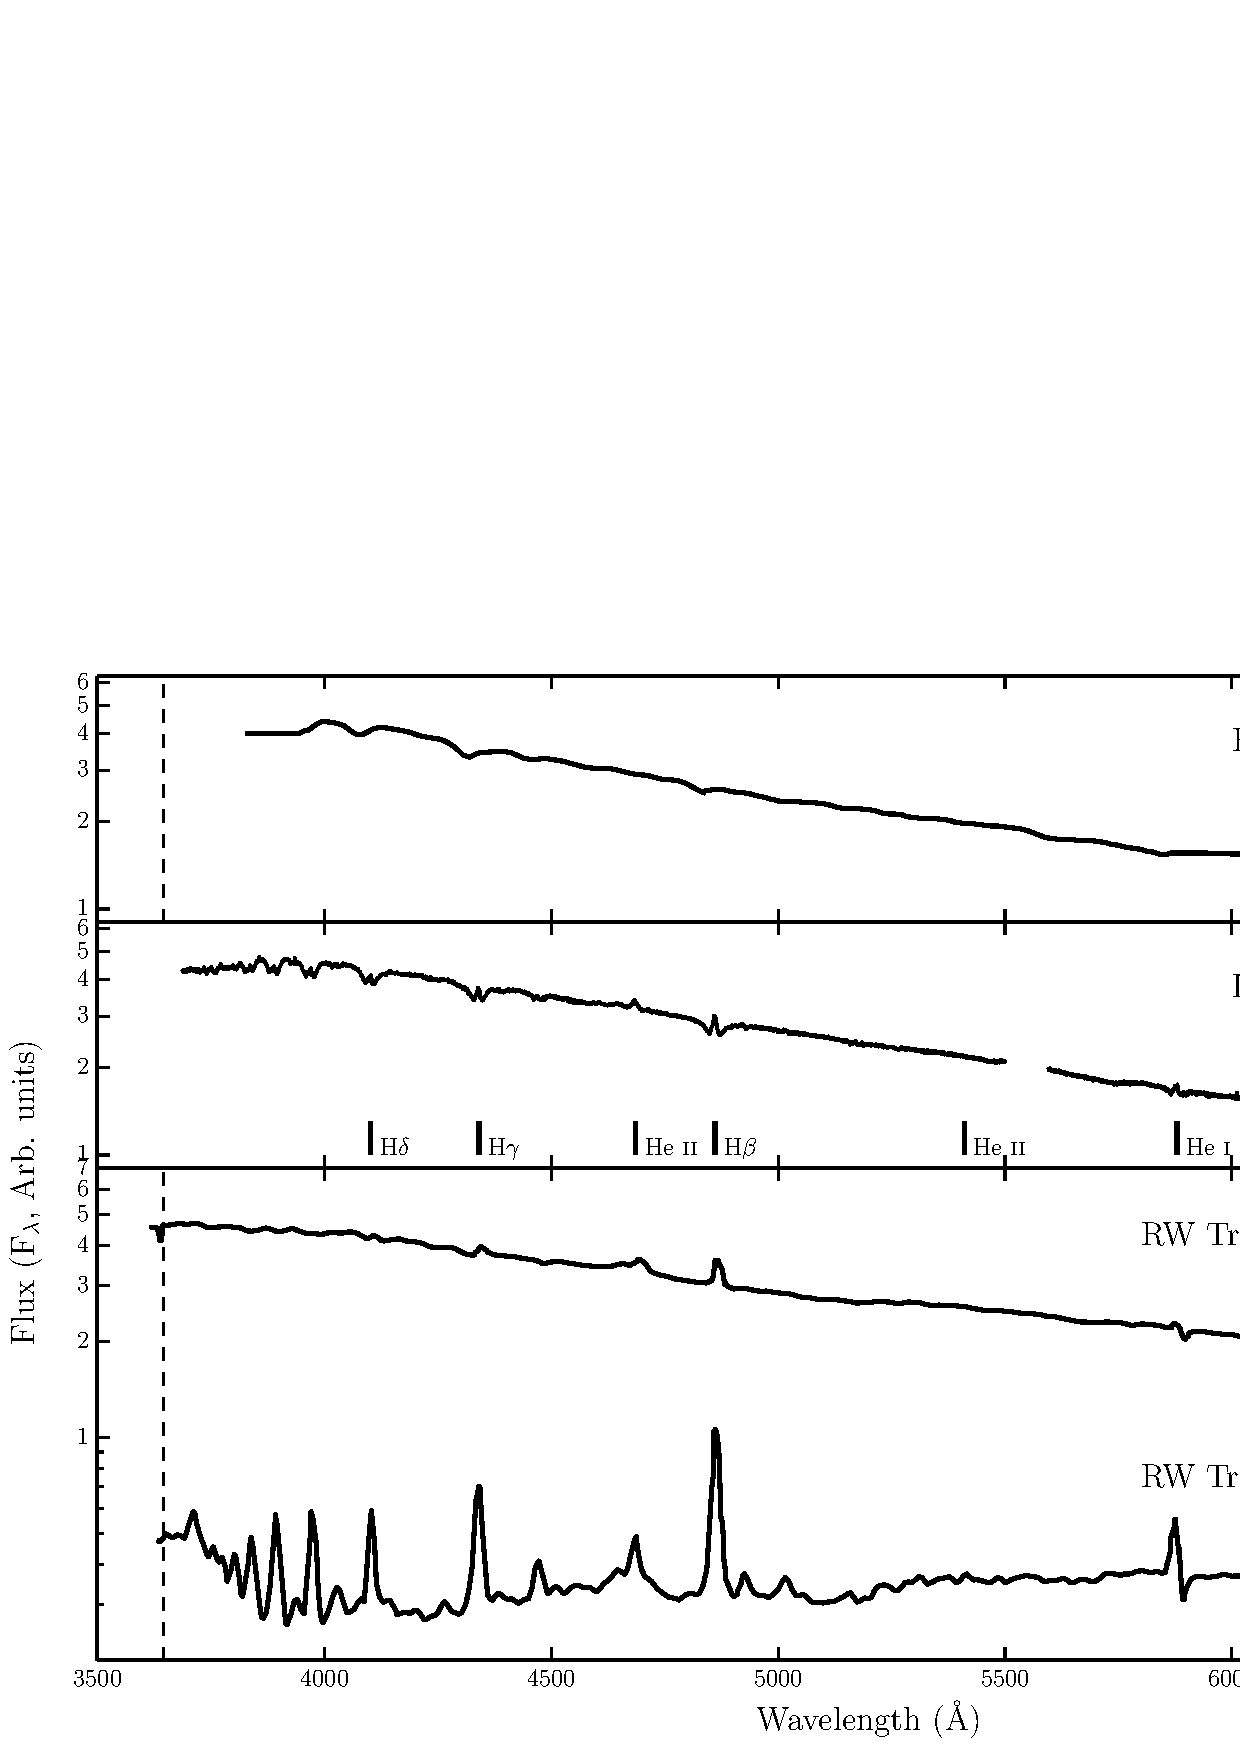
\includegraphics[width=1.0\textwidth]{figures/06-agnpaper/fig1.png}
\caption
[A cartoon showing the geometry and some key parameters of
the biconical quasar wind model.]
{
A cartoon showing the geometry and some key parameters of
the biconical quasar wind model.
}
\label{fig:cartoon_qso}
\end{figure} 

\subsection{Photon Sources}
\label{sec:photon_sources}

Two sources of r-packets are included in the model:
An accretion disc and a central X-ray s ce.
The accretion disc is assumed to be geometrically thin, 
but optically thick.
Accordingly, the disc is modelled as an ensemble of blackbodies with a 
\cite{shakurasunyaev1973} effective temperature profile. 
The emergent SED is then determined by the specified accretion rate ($\dot{M}$)
and central BH mass ($M_{BH}$).
All photon sources in the model are opaque, meaning
that r-packets that strike them are destroyed.
The inner radius of the disc extends to the innermost 
stable circular orbit (ISCO) of the BH. 
I assume a Schwarzchild BH with an ISCO at $6~r_G$, where 
$r_G = GM_{BH}/c^2$ is the gravitational radius.
For a $10^9~M_\odot$ BH, this is equal to $8.85\times10^{14}~{\rm cm}$ 
or $\sim10^{-4}~{\rm pc}$.  


The X-ray source is treated as an isotropic sphere at the ISCO,
which emits $r$-packets according to a power law in flux with index $\alpha_X$, of the form
\begin{equation}
F_X (\nu) = K_X \nu^{\alpha_X}.
\end{equation}
The normalisation, $K_X$ of this power law is such that it 
produces the specified 2-10~keV luminosity, $L_X$.
The input spectrum for the simulations is therefore a simple combination
of a power law X-ray component and accretion disc spectrum; an example input
spectrum is shown in Fig.~\ref{fig:qso_model_sed}. In actual fact, this
spectrum will be angle dependent due to the geometry of the system and 
the angular emissivity profile of the accretion disc (see sections~\ref{sec:xray}
and \ref{sec:ew_in_model}.
Photons, or $r$-packets, produced by the accretion disc and central X-ray source
are reprocessed by the wind. This reprocessing is dealt with by enforcing strict
radiative equilibrium ({\em modulo} adiabatic cooling; see section~\ref{sec:estimators})
via the indivisible energy packet constraint.  

\begin{figure} 
\centering
\includegraphics[width=1.0\textwidth]{figures/06-agnpaper/qso_model_sed.png}
\caption
[The input spectrum used for the quasar modelling.]
{
The input spectrum used for the quasar modelling.
}
\label{fig:qso_model_sed}
\end{figure} 

\subsection{A Simple Approximation for Clumping}

In previous modelling efforts with \py, a smooth outflow was assumed, 
such that the density at a given point was determined only by the 
kinematic parameters and mass loss rate. However, as already discussed,
AGN winds exhibit significant substructure -- the outflow is expected to be
{\em clumpy}, rather than smooth, and probably on a variety of scales. 
A clumpy outflow offers a possible solution to the so-called `over-ionization problem' in 
quasar and AGN outflows \citep[e.g.][]{junk1983,weymann1985,hamann2013}. 
This is the main motivation for incorporating clumping into the model.

Deciding on how to implement clumping into the existing wind models was not straightforward.
First, and most importantly, the physical scale lengths and density contrasts in AGN outflows are not well-constrained from observations or theory.  As a result, while one could envision in principle, clouds with a variety of sizes and density contrasts varying perhaps as function of radius, there would have been very little guidance on how to set nominal values of the various parameters of such a model.
Second, there are significant computational difficulties associated with adequately resolving and realistically modelling a series of small scale, high density regions with a MCRT
-- or for that matter, a hydrodynamical -- code. 
Given the lack of knowledge about the actual type of clumping, I have implemented
a simple approximation used successfully in stellar wind modelling, known as 
{\em microclumping} \citep[e.g.][]{hamann1998,hilliermiller1999,hamann2008}.  

The underlying assumption of microclumping is that clump sizes 
are much smaller than the 
typical photon mean free path, and thus the clumps are 
both geometrically and optically thin. This approach 
allows one to treat clumps only in terms of their volume filling factor, $f_V$, 
instead of having to specify separately their size and density distributions.
In this model, $f_V$ is independent of position.
The inter-clump medium is modeled as a vacuum,
although the outflow is still non-porous and axisymmetric.
This approach therefore assumes that the inter-clump medium
is unimportant in determing the output spectrum, which
is expected to be true only when density constrasts are large and
the inter-clump medium is both very ionized and of low emissivity and opacity.
The density of the clumps is multiplied by the ``density enhancement'' 
$D=1/f_V$. Opacities, $\kappa$, and emissivities, $j$, 
can then be expressed as 
\begin{equation}
\kappa = f_V \kappa_C(D);~~j = f_V j_C(D).
\end{equation}
Here the subscript $C$ denotes that the quantity is calculated using the 
enhanced density in the clump. The resultant effect is that, {\em for fixed temperature},
processes that are linear in density, such as electron scattering, are unchanged, 
as $f_V$ and $D$ will cancel out. However, any quantity that scales with the square of density, 
such as collisional excitation or recombination, will increase by a factor of $D$.
In \py, the temperature is not fixed, and is instead set by balancing heating and 
cooling in a given cell. In the presence of an X-ray source, this thermal balance is 
generally dominated by bound-free heating and line cooling. The main effect of including 
clumping in this modelling is that it moderates the ionization state due to the increased 
density. This allows an increase in the ionizing luminosity, amplifying the amount of
bound-free heating and also increasing the competing line cooling term
(thermal line emission).

The shortest length scale in a Sobolev MCRT treatment such as that used here
is normally the Sobolev length, given by
\begin{equation}
l_S = \frac{v_{th}}{| dv/ds |}
\end{equation}
This is typically $\sim10^{13}$~cm near the disc plane, increasing outwards.
The Sobolev length calculated from the mean velocity gradient in a cell
is shown, together with the size of the cell
and Thomson mean free path, in Fig.~\ref{fig:length_scales}.
The mean density is used to calculate the Sobolev optical depth, 
which assumes that $l_S$ is greater than the typical clump size.
Thus for the microclumping assumption to be formally correct, 
clumps should be no larger than $\sim10^{12}$~cm.
This size scale is not unreasonable for quasar outflows, as
\cite{dekool1995} suggest that BAL flows may have low filling factors with
clump sizes of $\sim10^{11}$~cm.
% An additional concern with this approach to clumping is that the clumps
% may rapidly cool and expand into the inter-clump medium. This is a well-known
% issue in BLR and outflow models (REFs), and requires some kind of confining mechanism,
% such as magnetic confinement \cite[e.g.][]{dekool1995}. Alternatively, as already discussed,
% the LDI may cause clumpy flows as expected in stellar winds.}
\begin{figure} 
\centering
\includegraphics[width=1.0\textwidth]{figures/06-agnpaper/size_of_clumps.png}
\caption
[Some typical length scales for the fiducial model.]
{
Some typical length scales for the fiducial model. 
This places a formal limit of $\sim10^{12}$~cm on clump sizes 
in the microclumping framework, and confirms that the cells are sufficiently
larger than the Sobolev length in almost all cases.
}
\label{fig:length_scales}
\end{figure} 

This clumping treatment is necessarily simple; it does not adequately
represent the complex substructures and stratifications in ionization
state expected in AGN outflows. 
Nevertheless, this parameterization 
allows simple estimates of the effect clumping has on the ionization 
state and emergent line emission.


\subsection{The Simulation Grid}
\label{sec:sim_grid}
Using this prescription, I conducted a limited parameter
search over a 5-dimensional parameter space involving the 
variables $r_{\mathrm{min}}$, $\theta_{\mathrm{min}}$, $f_V$, $\alpha$ and $R_v$.
The grid points are shown in table~\ref{grid_table}.
The aim here was to first fix $M_{BH}$ and $\dot{M}$ to their H13 values,
and increase $L_X$ to $10^{45}$~erg~s$^{-1}$ (a more realistic value for a 
quasar of $10^9~M_\odot$ and an Eddington fraction of $0.2$; see section~\ref{sec:xray}).

These models were then evaluated based on 
how closely their synthetic spectra reproduced the 
following properties of quasars and BALQSOs:

\begin{itemize}
\item UV absorption lines 
with $BI > 0$ at $\sim20\%$ of viewing angles \cite[e.g.][]{knigge2008};
\item Line emission emerging at low inclinations, with $\mathrm{EW}\sim40$~\AA\ in \civline\ \citep[e.g. ][]{shen2011};
\item H recombination lines with $EW\sim50$~\AA\ in \la\ \citep[e.g. ][]{shen2011};
\item  \mg\ and \al\ (LoBAL) absorption features with $BI > 0$ at a subset of 
BAL viewing angles;
\item Verisimilitude with quasar composite spectra.
\end{itemize}
Here $BI$ is the `Balnicity Index' (Weymann et al. 1991), given by
\begin{equation}
BI = \int^{25000~{\rm km~s}^{-1}}_{3000~{\rm km~s}^{-1}} C \left( 1 - \frac{f(v)}{0.9} \right) dv.
\end{equation}
The constant $C=0$ everywhere, unless the normalized flux
has satisfied $f(v)<0.9$ continuously for at least $2000$~km~s$^{−1}$, 
whereby $C$ is set to $1$.

In the next section, I present one of the most promising models,
which I refer to as the fiducial model, and discuss
the various successes and failures with respect to the above criteria.
This allows insight into fundamental geometrical 
and physical constraints to be gained, 
and the potential for unification assessed. 
I then discuss the sensitivity to key parameters in section~\ref{sec:param_sens}.
The full grid, including output synthetic spectra and plots can be found at
\url{jhmatthews.github.io/quasar-wind-grid/}.

\begin{table}
\centering
\begin{tabular}{p{2cm}p{1cm}p{1cm}p{1cm}p{1cm}}
Parameter & \multicolumn{4}{l}{Grid Point Values}  \\
\hline \hline 
$r_{\mathrm{min}}$ 	&	 $60r_{g}$ & $180r_{g}$ & \multicolumn{2}{l}{$300r_{g}$} \\ 
$\theta_{\mathrm{min}}$ 	& $55^{\circ}$ & \multicolumn{3}{l}{$70^{\circ}$} \\ 
$R_v$  	        &	 $10^{18}$~cm & \multicolumn{3}{l}{$10^{19}$~cm} \\ 
$\alpha$ 	&	 $0.5$ & $0.6$ & $0.75$ & $1.5$ \\
$f_V$ 	&	 $0.01$ & \multicolumn{3}{l}{$0.1$}  \\
\hline 
\end{tabular}
\caption
[The grid points used in the parameter search for quasar wind models]
{The grid points used in the parameter search.
The sensitivity to some of these parameters is discussed 
further in section~\ref{sec:param_sens}}
\label{grid_table}
\end{table}



%%%%%%%%%%%%%%%%%%%%%%%%%%%%%%%%%%%%%%%%%%%%%%%%%

% RESULTS

%%%%%%%%%%%%%%%%%%%%%%%%%%%%%%%%%%%%%%%%%%%%%%%%%


\section{Results and Analysis from a Fiducial Model}
\label{sec:qso_results}
Here I describe the results from a fiducial model,
and discuss these results in the context of the criteria 
presented in section~\ref{sec:sim_grid}. 
The parameters of this model are shown in table~\ref{wind_param}.
Parameters differing from the benchmark model of H13 are 
highlighted with an asterisk. In this section, I examine the physical 
conditions of the flow, and present the synthetic spectra, before comparing
the X-ray properties of this particular model to samples of
quasars and luminous AGN. 

\begin{table}
\centering
\begin{tabular}{p{3cm}p{4cm}}
\hline Parameter 	&	 Value \\ 
\hline \hline 
$M_{BH}$ 	 &	 $1\times 10^9~\rm{M_{\odot}}$ \\ 
$\dot{M}_{\mathrm{acc}}$ 	 &	 $5~M_{\odot}\mathrm{yr}^{-1} \simeq 0.2~\dot{M}_{\mathrm{Edd}}$\\ 
$\alpha_X$ 	 &	 $-0.9$ \\ 
$L_{X} $ 	 &	 $10^{45}~\rm{erg~s^{-1}}$$^*$ \\ 
$r_{\mathrm{disc}}(\mathrm{min})=r_{X}$   &	 $6r_g=8.8\times10^{14}~{\rm cm}$ \\ 
$r_{\mathrm{disc}}(\mathrm{max})$   &	 $3400r_g = 5\times10^{17}~{\rm cm}$ \\ 
$\dot{M}_W$  &	 $5~M_{\odot}yr^{-1}$ \\ 
$r_{\mathrm{min}}$ 	&	 $300r_{g} = 4.4\times10^{16}~{\rm cm}$\\ 
$r_{\mathrm{max}}$ 	&	 $600r_{g} = 8.8\times10^{16}~{\rm cm}$ \\ 
$\theta_{\mathrm{min}}$ 	&	 $70.0^{\circ}$ \\ 
$\theta_{\mathrm{max}}$ 	&	 $82.0^{\circ}$ \\ 
%%$\lambda$ 	&	 $0$ \\ 
$v_{\infty}(r_0)$ 	&	 $v_{\mathrm{esc}}(r_0)$ \\ 
$R_v$  	        &	 $10^{19}$~cm$^*$ \\ 
$\alpha$ 	&	 $0.5^*$ \\
$f_V$ 	&	 $0.01^*$  \\
$n_x$ 	&	 $100$  \\
$n_z$ 	&	 $200$  \\
\hline 
\end{tabular}
\caption
[Model parameters for the fiducial quasar model.]
{Wind geometry parameters 
used in the fiducial model, as defined in the text and Fig.~\ref{fig:cartoon_qso}.
Parameters differing from the benchmark model of H13 are 
highlighted with an asterisk.}
\label{wind_param}
\end{table}



\subsection{Physical Conditions and Ionization State}


\begin{figure*}
\centering
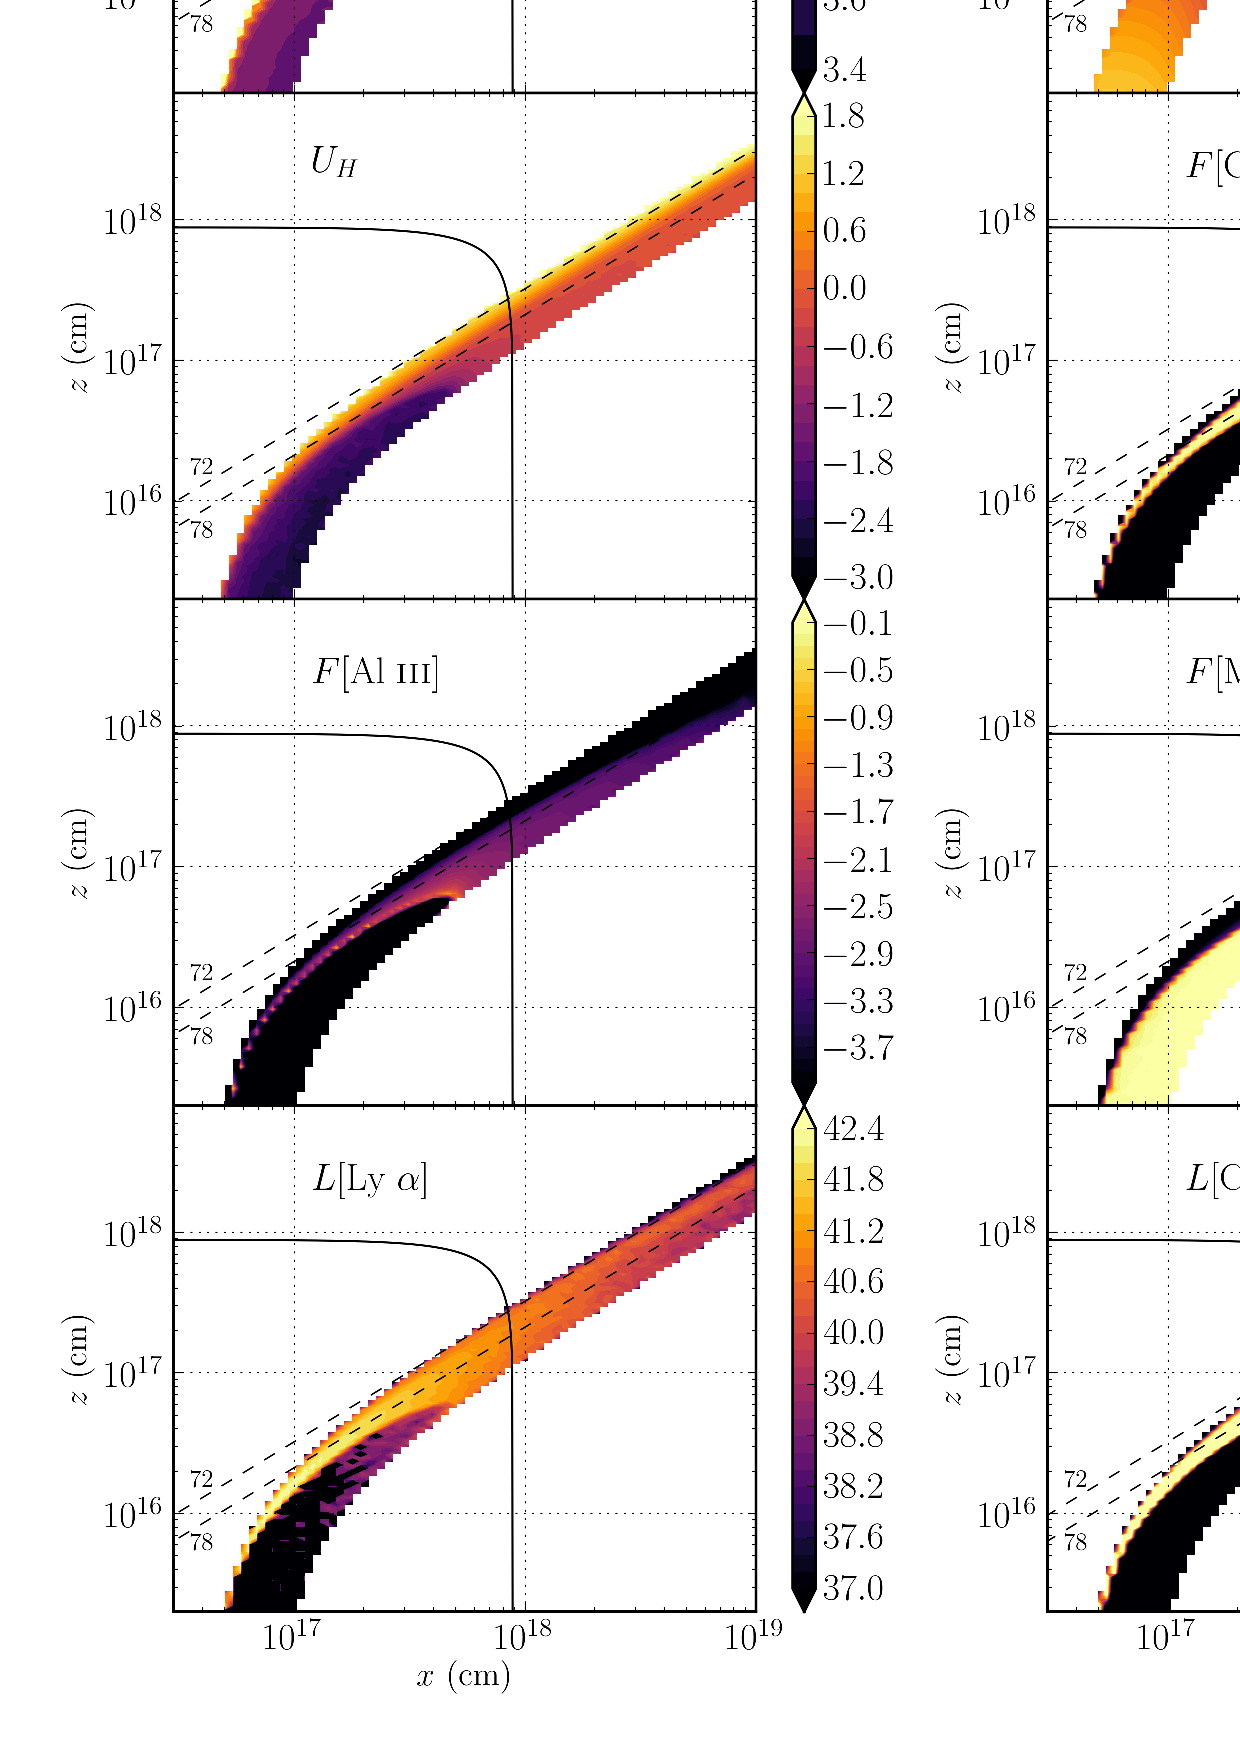
\includegraphics[width=1.0\textwidth]{figures/06-agnpaper/fig2.png}
\caption
[Contour plots showing the logarithm of some important 
physical properties of the quasar outflow.]
{
Contour plots showing the logarithm of some important 
physical properties of the outflow. The spatial scales are
logarithmic and the $x$ and $z$ scales are not the same.
Symbols are defined in the text.
The solid black line marks a sphere at $1000~r_G$.
The dotted lines show the $72^\circ$ and $78^\circ$ sightlines 
to the centre of the system, and illustrate that different sightlines
intersect material of different ionization states.
The line luminosities, $L$, represent the luminosity of photons
escaping the Sobolev region for each line. These photons do not
necessarily escape to infinity.
}
\label{fig:wind}
\end{figure*}

\begin{figure} 
\centering
\includegraphics[width=0.8\textwidth]{figures/06-agnpaper/ne_in_wind.png}
\caption
[The electron density in the fiducial model on linear axes.]
{
The electron density in the model, this time on linear axes
in order to illustrate the density contrasts and scale of the system.
The plot is on the scale of the acceleration length, whereas
the inset is a box of $2700 \times 800 r_G$, where the bottom left corner
corresponds to the base of the innermost streamline.
}
\label{fig:ne_in_wind}
\end{figure} 

\noindent
Fig.~\ref{fig:wind} shows the physical properties of the wind.
The wind rises slowly from the disc at first, with densities within clumps
of $n_H \sim 10^{11}~\rm{cm^{-3}}$ close to the disc plane, 
where $n_H$ is the local number density of H. To illustrate the degree
of scale and density ranges in the model I also show $n_e$ in the wind
on a linear scale in Fig.~\ref{fig:ne_in_wind}.
The flow then accelerates over a scale length of $R_V=10^{19}~\rm{cm}$
up to a terminal velocity equal to the escape velocity at the streamline base
($\sim10,000~\rm{km~s^{-1}}$). This gradual acceleration results in
a wind that exhibits a stratified ionization structure, with low ionization material
in the base of the wind giving way to highly ionized plasma further out.
This is illustrated in Fig.~\ref{fig:wind} 
by the panels showing the ion fraction $F=n_j/n_{tot}$ of some important ions.
The clumped wind produces the range of ionization states observed
in quasars and BALQSOs, while adopting a realistic $2-10$ keV X-ray luminosity
of $L_{X}=10^{45}~\rm{erg~s^{-1}}$. Without clumping, this wind would be over-ionized 
to the extent that opacities in e.g., \civ\ would be entirely negligible (see H13).

One common way to quantify the ionization state of a plasma
is through the ionization parameter, $U_H$, given by equation~\ref{eq:ip}.
Shown in Fig.~\ref{fig:wind},
the ionization parameter is a useful measure of the global ionization state,
as it represents the ratio of the number density of 
H ionizing photons to the local H density.
It is, however, a poor representation of the 
ionization state of species such as \civ\ as it encodes no information
about the shape of the SED. In this case, the X-ray photons 
are dominant in the photoionization of the UV resonance line ions. 
This explains why a factor of 100 increase in X-ray luminosity requires
a clumping factor of 0.01, even though the value of $U_H$ decreases by only a factor of $\sim10$ compared to H13. 

The total line luminosity also increases dramatically compared to the unclumped model
described by H13. This is because the denser outflow can absorb the increased
X-ray luminosity without becoming over-ionized, leading to a hot plasma which
produces strong collisionally excited line emission.
This line emission typically emerges on the edge of the wind
nearest the central source. The location of the line emitting regions
is dependent on the ionization state, as well as the incident X-rays.
The radii of these emitting regions is important,
and can be compared to observations. The line luminosities, $L$,
shown in the figure correspond to the luminosity in $\LUM$ of photons
escaping the Sobolev region for each line. 
As shown in Fig.~\ref{fig:wind},
the \civline\ line in the fiducial model is typically formed between 
$100-1000~r_G$ ($\sim10^{17}-10^{18}~\rm{cm}$).
This is in rough agreement with the reverberation mapping 
results of \cite{kaspi2007} 
for the $2.6\times10^{9} M_\odot$ quasar S5 0836+71,
and also compares favourably with microlensing measurements of the size of the
\civline\ emission line region in the BALQSO H1413+117 \citep{odowd2015}.


\subsection{Synthetic Spectra: Comparison to Observations}

\begin{figure*}
\centering
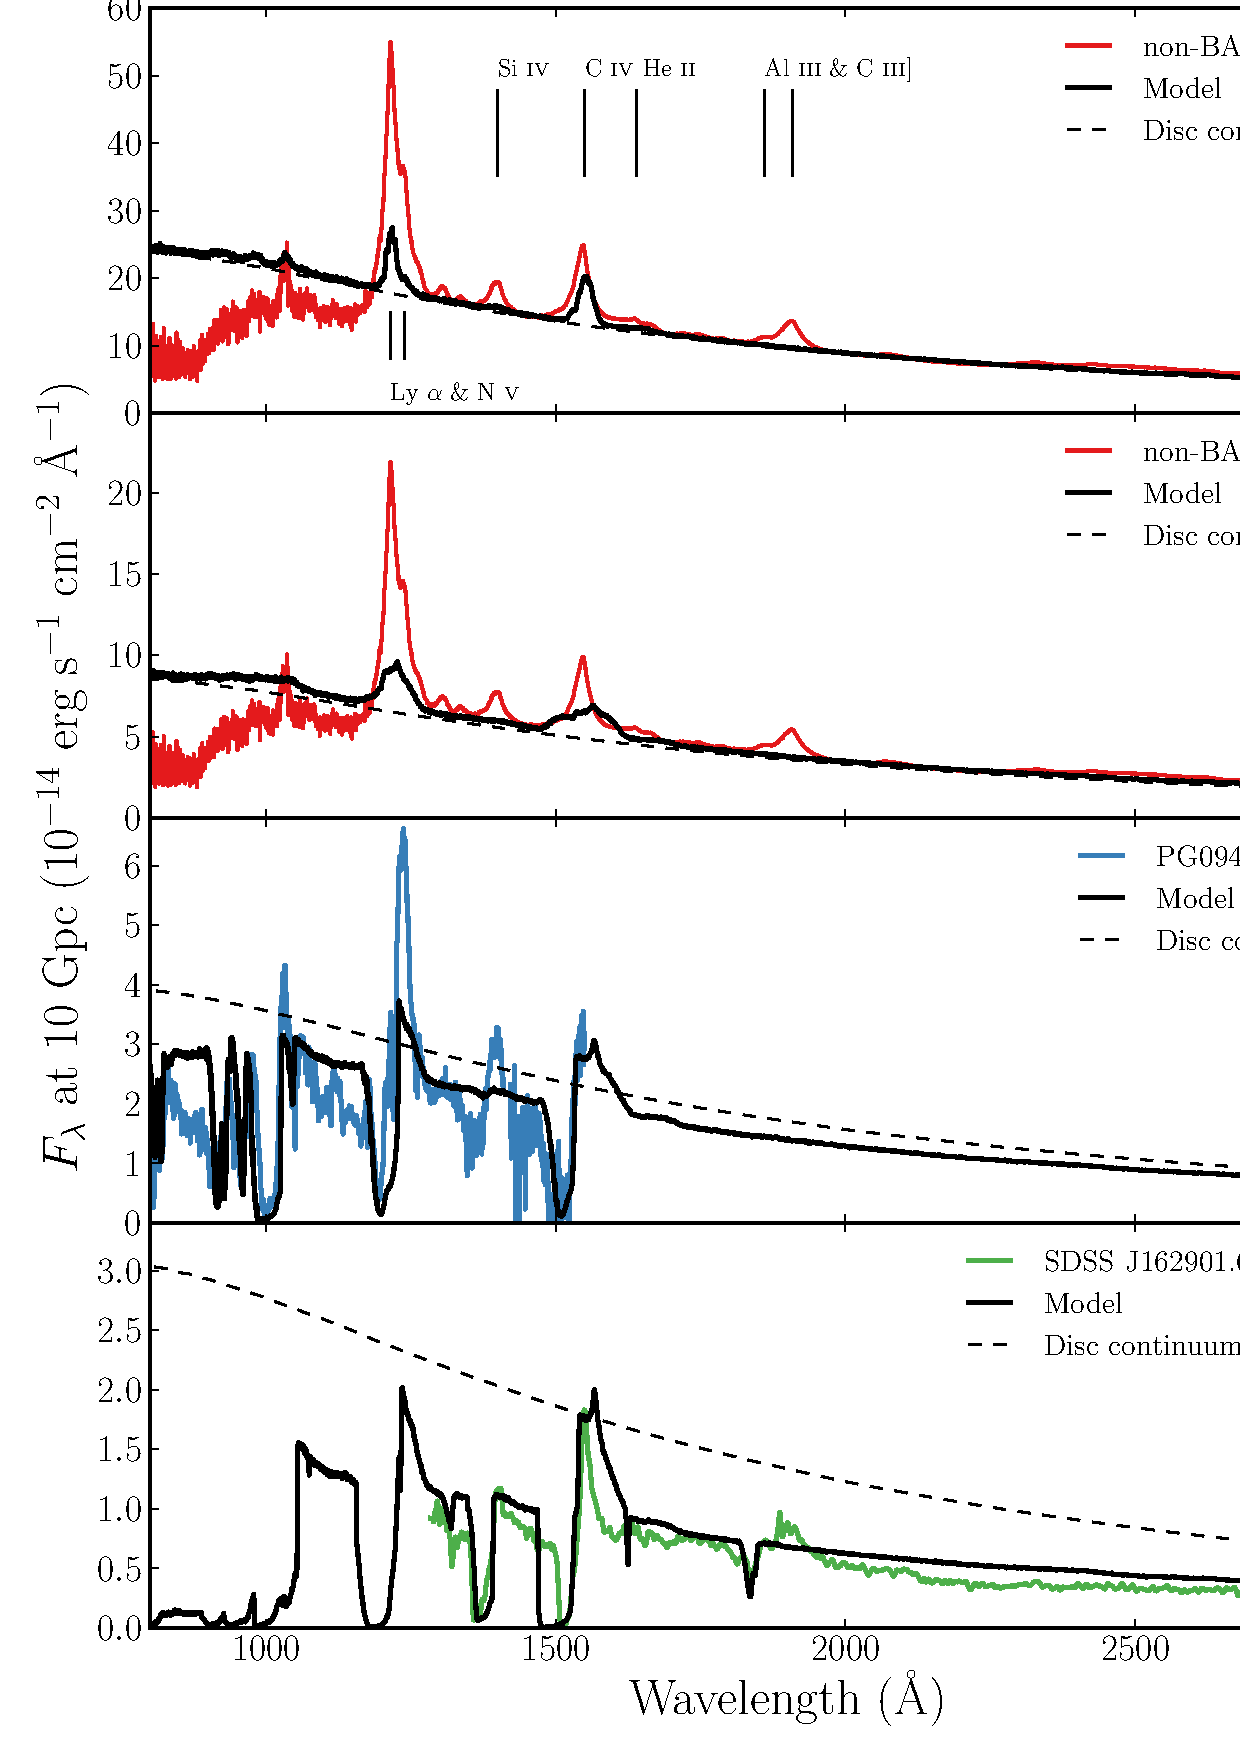
\includegraphics[width=1.0\textwidth]{figures/06-agnpaper/fig3.png}
\caption
[Synthetic spectra at four viewing angles for the fiducial quasar model.]
{
Synthetic spectra at four viewing angles for the fiducial model. At 
$20^\circ$ and $60^\circ$ I show a comparison to an SDSS quasar composite
from Recihard et al. (2003). At $73^\circ$ and $76^\circ$ I show a comparison to
an {\sl HST} STIS spectrum of the high BALnicity BALQSO 
PG0946+301 (Arav et al. 2000), and an SDSS spectrum of the LoBAL quasar 
SDSS J162901.63+453406.0, respectively. The dotted line shows a disc
only continuum to show the effect of the outflow on the continuum level. 
All the spectra are scaled to the model flux at $2000$~\AA, expect for the 
{\sl HST} STIS spectrum of PG0946+301, which is scaled to $1350$~\AA\
due to the incomplete wavelength coverage.
% HST STIS spectrum of PG0946+301 (Arav et al. 2000)
}
\label{fig:uvspec}
\end{figure*}

\begin{figure} 
\centering
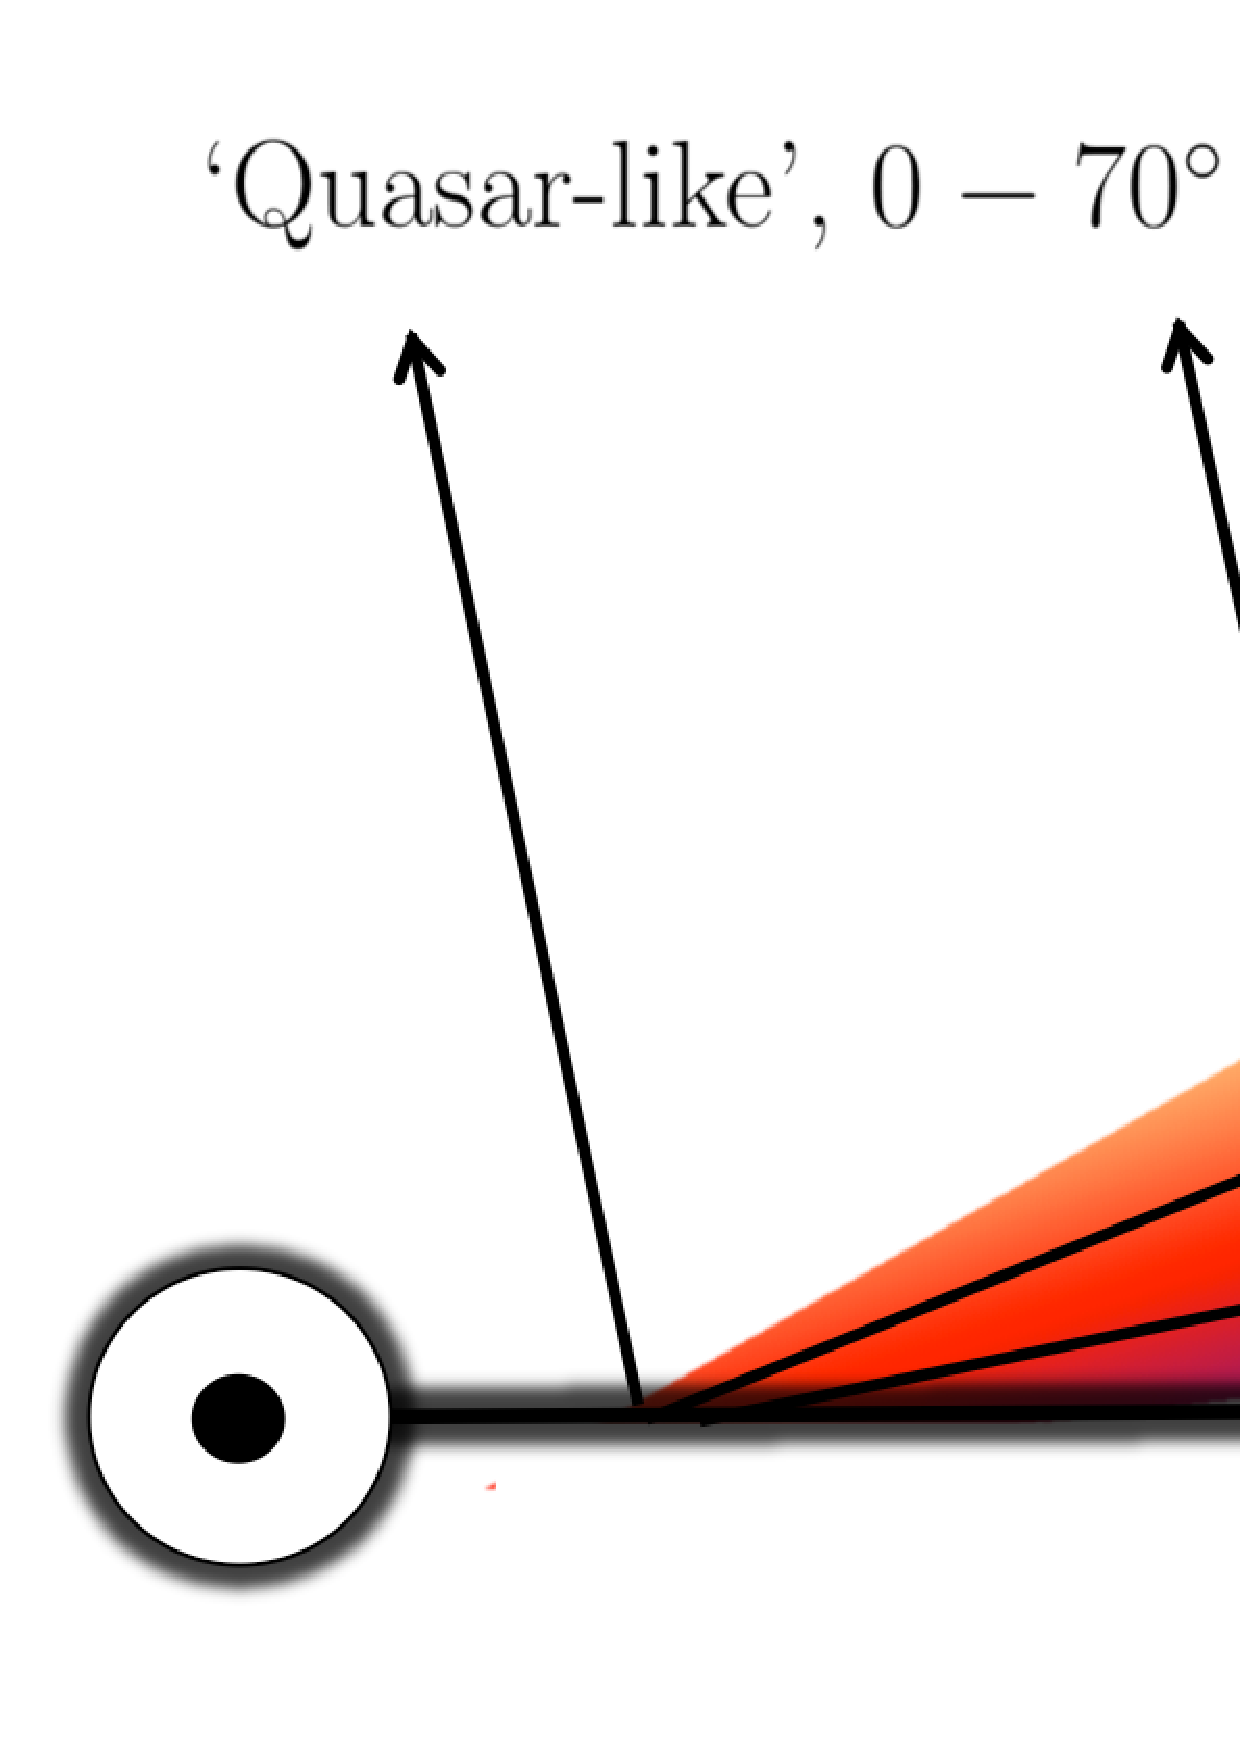
\includegraphics[width=1.0\textwidth]{figures/06-agnpaper/fig4.png}
\caption
[A schematic showing the broad classes of sightline 
in the fiducial model.]
{
A cartoon describing the broad classes of sightline 
in the fiducial model, illustrating how geometric effects lead to 
the different emergent spectra. The colour gradient is approximate,
but indicates the stratified ionization structure, 
from highly ionized (yellow) to low ionization (purple) material.
%[FIGURE NEEDS IMPROVING]
}
\label{fig:sightline}
\end{figure} 

\begin{figure*}
\centering
\includegraphics[width=0.9\textheight, angle=270]
{figures/06-agnpaper/fig5.png}
\caption
[Synthetic spectra at two viewing angles compared to the non-BAL SDSS quasar composite.]
{
Synthetic spectra at two viewing angles, 
this time in frequency space and including the optical band,
compared to the non-BAL SDSS quasar composite. The spectra are normalised to the flux at 
$2000$~\AA, then an offset of 2 is applied per spectrum for clarity -- the dotted lines show the zero point of $F_\nu / F_{2000}$ in each case.
}
\label{fig:sed}
\end{figure*}

\noindent
Fig.~\ref{fig:uvspec} shows the synthetic spectrum in the UV from the fiducial model. 
To assess the ability of the synthetic spectra to match real 
quasar spectra, I also show {\sl Sloan Digital Sky Survey} (SDSS) quasar
composites from \cite{reichard2003}, normalised to the flux at 2000~\AA\
for low inclinations. Unfortunately, the wide variety of
line profile shapes and internal trough structure in BALQSOs
tends to `wash out' BAL troughs in composite spectra
to the extent that BALQSO composites do not resemble typical BALQSOs.
Because of this, I instead compare to a {\sl Hubble Space Telescope} 
STIS spectrum of the high BALnicity BALQSO PG0946+301 (Arav et al. 2000),
and an SDSS spectrum of the LoBAL quasar SDSS J162901.63+453406.0,
for the angles of $73^\circ$ and $76^\circ$, respectively. 
A cartoon illustrating how geometric effects determine
the output spectra is shown in Fig.~\ref{fig:sightline}.  

\subsubsection{Broad Absorption Lines (`BALQSO-like' angles)}
\label{sec:balqso_angles}

The UV spectrum is characterised by strong BAL 
profiles at high inclinations ($> 70^\circ$). 
This highlights the first success of the model: 
clumping allows the correct ionization state 
to be maintained in the presence of strong X-rays, 
resulting in large resonance line opacities. 
At the highest inclinations, the 
cooler, low ionization material at the base of the wind
starts to intersect the line of sight. This produces 
multiple absorption lines in species such as \mg,
\al\ and Fe~\textsc{ii}. The potential links to LoBALQSOs and 
FeLoBALQSOs are discussed in section~\ref{sec:lobal}.

The high ionization BAL profiles are often saturated, and the location in velocity space
of the strongest absorption in the profile varies with inclination.
At the lowest inclination BAL sight lines, the strongest absorption occurs at the red edge,
whereas at higher inclinations (and for the strongest BALs)
the trough has a sharp edge at the terminal velocity.
This offers one potential explanation for the wide range of BALQSO absorption
line shapes \citep[see e.g.][]{trump2006,knigge2008,filizak2014}.

The absorption profiles seen in BALQSOs are often non-black, but saturated, 
with flat bases to the absorption troughs \citep{arav1999b,arav1999a}.
This is usually explained either as  partial covering of the continuum
source or by scattered contributions to the BAL troughs, necessarily
from an opacity source not co-spatial with the BAL forming region.
The scattered light explanation is supported by spectropolarimetry results
\citep{lamy2000}. The synthetic spectra do not show non-black, saturated profiles.
Black, saturated troughs are seen at angles $i > 73^\circ$, and the BALs
are non-saturated at lower inclinations. The reasons for this are inherent 
in the construction of the model. 
First, the microclumping assumption does not allow for 
porosity in the wind, meaning that it does not naturally produce
a partial covering absorber. To allow this, an alternative approach
such as {\em macroclumping} would be required \citep[e.g.][]{hamann2008,surlan2012}.
Second, the wind does not have a significant scattering contribution 
along sightlines which do not pass through the BAL region,
meaning that any scattered component to the BAL troughs is absorbed by line opacity.
This suggests that either the scattering cross-section of the wind must
be increased (with higher mass loss rates or covering factors), or 
that an additional source of electron opacity is required, potentially
in a polar direction above the disc. I note the scattering contribution
from plasma in polar regions is significant in some `outflow-from-inflow'
simulations \citep{KP09, simproga2012}.

\subsubsection{Broad Emission Lines (`quasar-like' angles)}

\begin{table}
\centering
\begin{tabular}{p{2cm}p{2cm}p{3cm}}
\hline Property & Synthetic, $20^\circ$ & Observed  (S11) \\ 
\hline \hline
$\log L$[C~\textsc{iv}]  & $44.60$ & $44.42 \pm 0.32$  \\
$\log L$[Mg~\textsc{ii}] & $43.92$ & $43.54 \pm 0.28$  \\
$\log (\nu L_{\nu})_{1350}$  & $46.42$ & $46.01 \pm 0.30$ \\
$\log (\nu L_{\nu})_{3000}$  & $46.18$ & $45.79 \pm 0.30$ \\
\hline
\end{tabular}
\caption
[Some derived spectral properties of the fiducial model compared to observations.]
{
Some derived spectral properties of the fiducial model, at $20^\circ$,
compared to observations. The observed values are taken from the Shen et al. (2011)
SDSS DR7 Quasar catalog, and correspond to mean values with standard deviations in log space
from a subsample with $8.5>\log(M_{BH})<9.5$ and 
$-1.5<\log (L_{\mathrm{bol}}/L_{\mathrm{Edd}}) < 0$,
where the BH mass is a \civ\ virial estimate. 
Units are logarithms of values in erg~s$^{-1}$.
%unless stated.otherwise.
}
\label{line_lums}
\end{table}


Unlike H13, significant collisionally excited line emission now emerges
at low inclinations in the synthetic spectra, particular in the \civ\ and \nv\
lines. Strong \la\ and
weak He~\textsc{ii}~$1640$~\AA\ lines are also observed
as a result of the improved treatment of recombination using macro-atoms. 
In the context of unification, this is a promising result, 
and shows that a biconical wind can produce significant 
emission at `quasar-like' angles. To demonstrate this further,
I show line luminosities and monochromatic continuum luminosities
from the synthetic spectra in table~\ref{line_lums}. These are compared to
mean values from a subsample of the SDSS DR7 quasar catalog \citep{shen2011} 
with BH mass and Eddington fraction estimates similar to the fiducial model values 
(see caption). The spectra do not contain the strong 
C~\textsc{iii}]~1909~\AA\ line seen in the quasar composite spectra, 
but this is due to a limitation of the current treatment of C; semi-forbidden
(intercombination) lines are not included in this modelling.

In Fig.~\ref{fig:sed}, I show an $F_{\nu}$ spectrum with broader waveband coverage
that includes the optical, showing that the synthetic spectra 
also exhibit \ha\ and \hb\ emission. 
In this panel, I include a low inclination and 
also a very high inclination 
spectrum, which looks underneath the wind cone. This model shows 
strong line emission with very similar widths and line ratios to the quasar composites, and
the Balmer lines are double peaked, due to velocity projection effects.  
Such double-peaked lines are seen in so-called `disc emitter' systems 
\citep[e.g.][]{eracleous1994} but not the majority of AGN.     
The line equivalent widths (EWs) increase at high inclination
due to a weakened continuum from wind attenuation, 
disc foreshortening and limb darkening. This effect also 
leads to a redder continuum slope, as seen in quasars, which is
due to Balmer continuum and Balmer and Fe~\textsc{ii} line emission.
This extreme $89^\circ$ viewing angle cannot represent a typical quasar within a unified model,
but does show that a model such as this can naturally reproduce quasar emission lines
if the emissivity of the wind is increased {\em with respect to the disc continuum}.
In addition, it neatly demonstrates how a stratified outflow can naturally
reproduce the range of ionization states seen in quasars. 

Despite a number of successes, 
there are a some properties of the synthetic spectra
that are at odds with the observations. First, the ratios of the 
EW of the \la\ and \mgline\ lines
to the EW of \civline\ are much lower than in the composite spectra. 
Similar problems have also been seen in simpler photoionization models for the 
BLR \citep{netzer1990}.
It may be that a larger region of very dense ($n_e\sim10^{10}$cm$^{-3}$) 
material is needed, which could correspond to a disc atmosphere or 
`transition region' 
\citep[see e.g.][]{MCGV95,knigge1998}. \nocite{knigge1998} 
While modest changes to geometry may permit this, the initial grid search 
did not find a parameter space in which the \la\ or \mg\ EWs
were significantly higher (see section~\ref{sec:param_sens}). 
Second, EWs increase with inclination 
(see Fig.~\ref{fig:uvspec} and Fig.~\ref{fig:sed}; also Fig.~\ref{fig:lobal}).
This is discussed further in section~\ref{sec:ew_in_model}.

\subsection{X-ray Properties}
\label{sec:xray}


\begin{figure*}
\centering
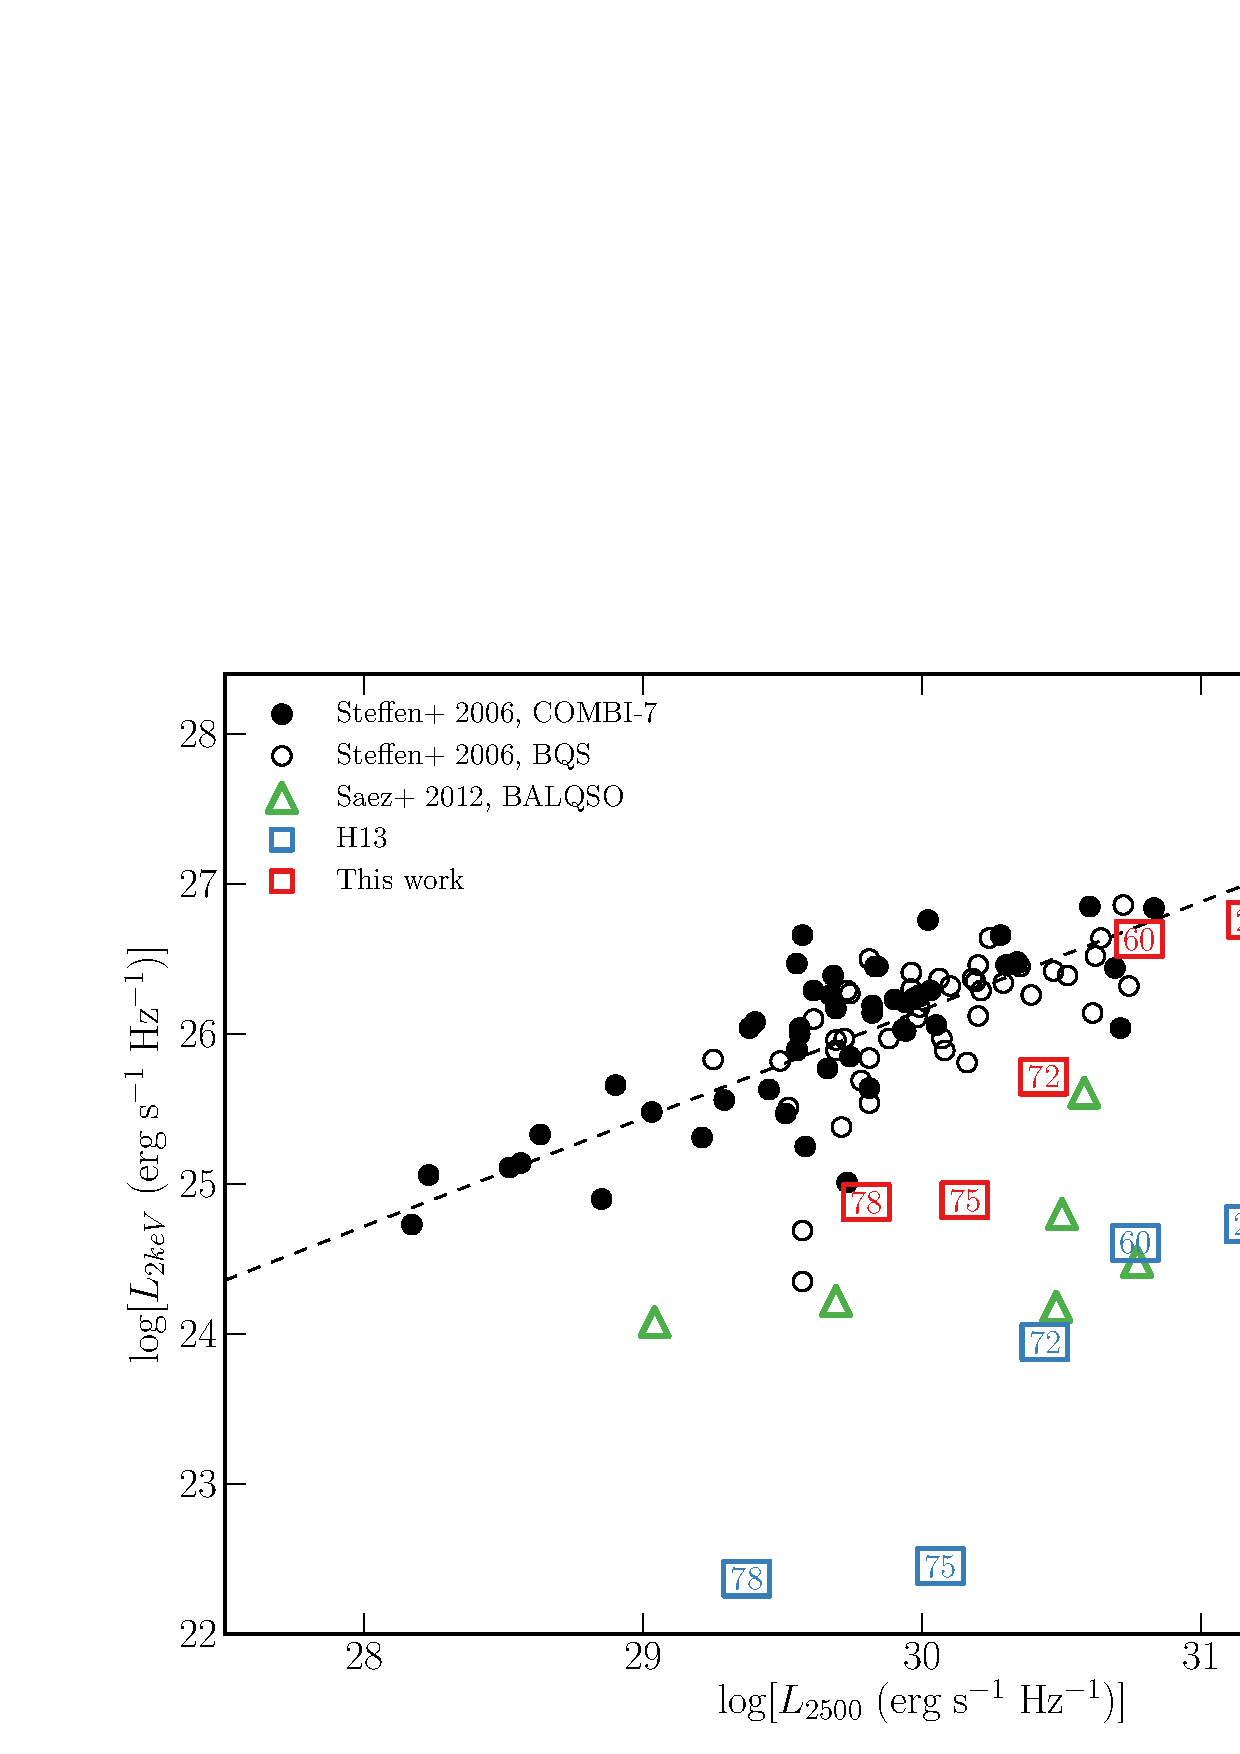
\includegraphics[width=1.0\textwidth]{figures/06-agnpaper/fig6.png}
\caption
[X-ray properties of the clumped quasar model compared to H13 and samples
from the literature.]
{
X-ray ($2$~keV) luminosity of the clumped model (red squares) 
and the H13 model (blue squares), plotted against monochromatic luminosity 
at 2500~\AA. The points are labeled according to inclination; angles
$>70^\circ$ correspond to BALs in this scheme (see Fig.~\ref{fig:sightline}).
Also plotted are masurements from 
the COMBI-7 AGN and the BQS samples (Steffen et al. 2006) and the Saez et al. (2012) 
sample of BALQSOs. The dotted line shows the best fit relation for non-BALQSOs 
from Steffen et al. (2006).
}
\label{fig:xray}
\end{figure*}

The main motivation for adding clumping to the model was
to avoid over-ionization of the wind in the presence of strong X-rays. 
Having verified that strong BALs appear in the synthetic spectra,
it is also important to assess whether the X-ray properties of this
fiducial model agree well with quasar and BALQSO samples for the relevant
inclinations.

Fig.~\ref{fig:xray} shows the emergent
monochromatic luminosity ($L_\nu$) at 2~keV and 
plotted against $L_\nu$ at $2500$~\AA\ 
for a number of different viewing angles in the model.
The monochromatic luminosities are calculated from the synthetic spectra and thus include
the effects of wind reprocessing and attenuation. In addition to model outputs,
I also show the BALQSO sample of Saez et al. (2012) and luminous AGN and quasar
samples from Steffen et al. (2006). The best fit relation from Steffen et al. (2006) 
is also shown. For low inclination, `quasar-like' viewing angles,
the model properties are in excellent agreement with AGN samples. The slight gradient from $20^\circ$ to
$60^\circ$ in the models is caused by a combination of disc foreshortening and limb-darkening 
(resulting in a lower $L_{2500}$ for higher inclinations), and the fact that the disk 
is opaque, and thus the X-ray source subtends a smaller solid angle at high inclinations
(resulting in a lower $L_{2keV}$ for higher inclinations). 


The high inclination, `BALQSO-like' viewing angles show moderate agreement with the data,
and are X-ray weak due to bound-free absorption and electron scattering in the wind.
Typically, BALQSOs show strong X-ray absorption with columns 
of $N_H\sim10^{23}~\rm{cm^{-2}}$ 
\citep{green1996,mathur2000,green2001,grupemathur2003}.
This is often cited as evidence that the BAL outflow is shielded from
the X-ray source, especially as sources with strong X-ray absorption tend
to exhibit deep BAL troughs and high outflow velocities 
\citep{brandt2000,laorbrandt2002,gallagher2006}.
These results imply that the clumpy BAL outflow
itself can be responsible for the strong X-ray absorption, 
and supports the suggestion of \cite{hamann2013} that 
geometric effects explain the weaker X-ray absorption in mini-BALs 
compared to BALQSOs.

\subsection{LoBALs and Ionization Stratification}
\label{sec:lobal}
\begin{figure*}
\centering
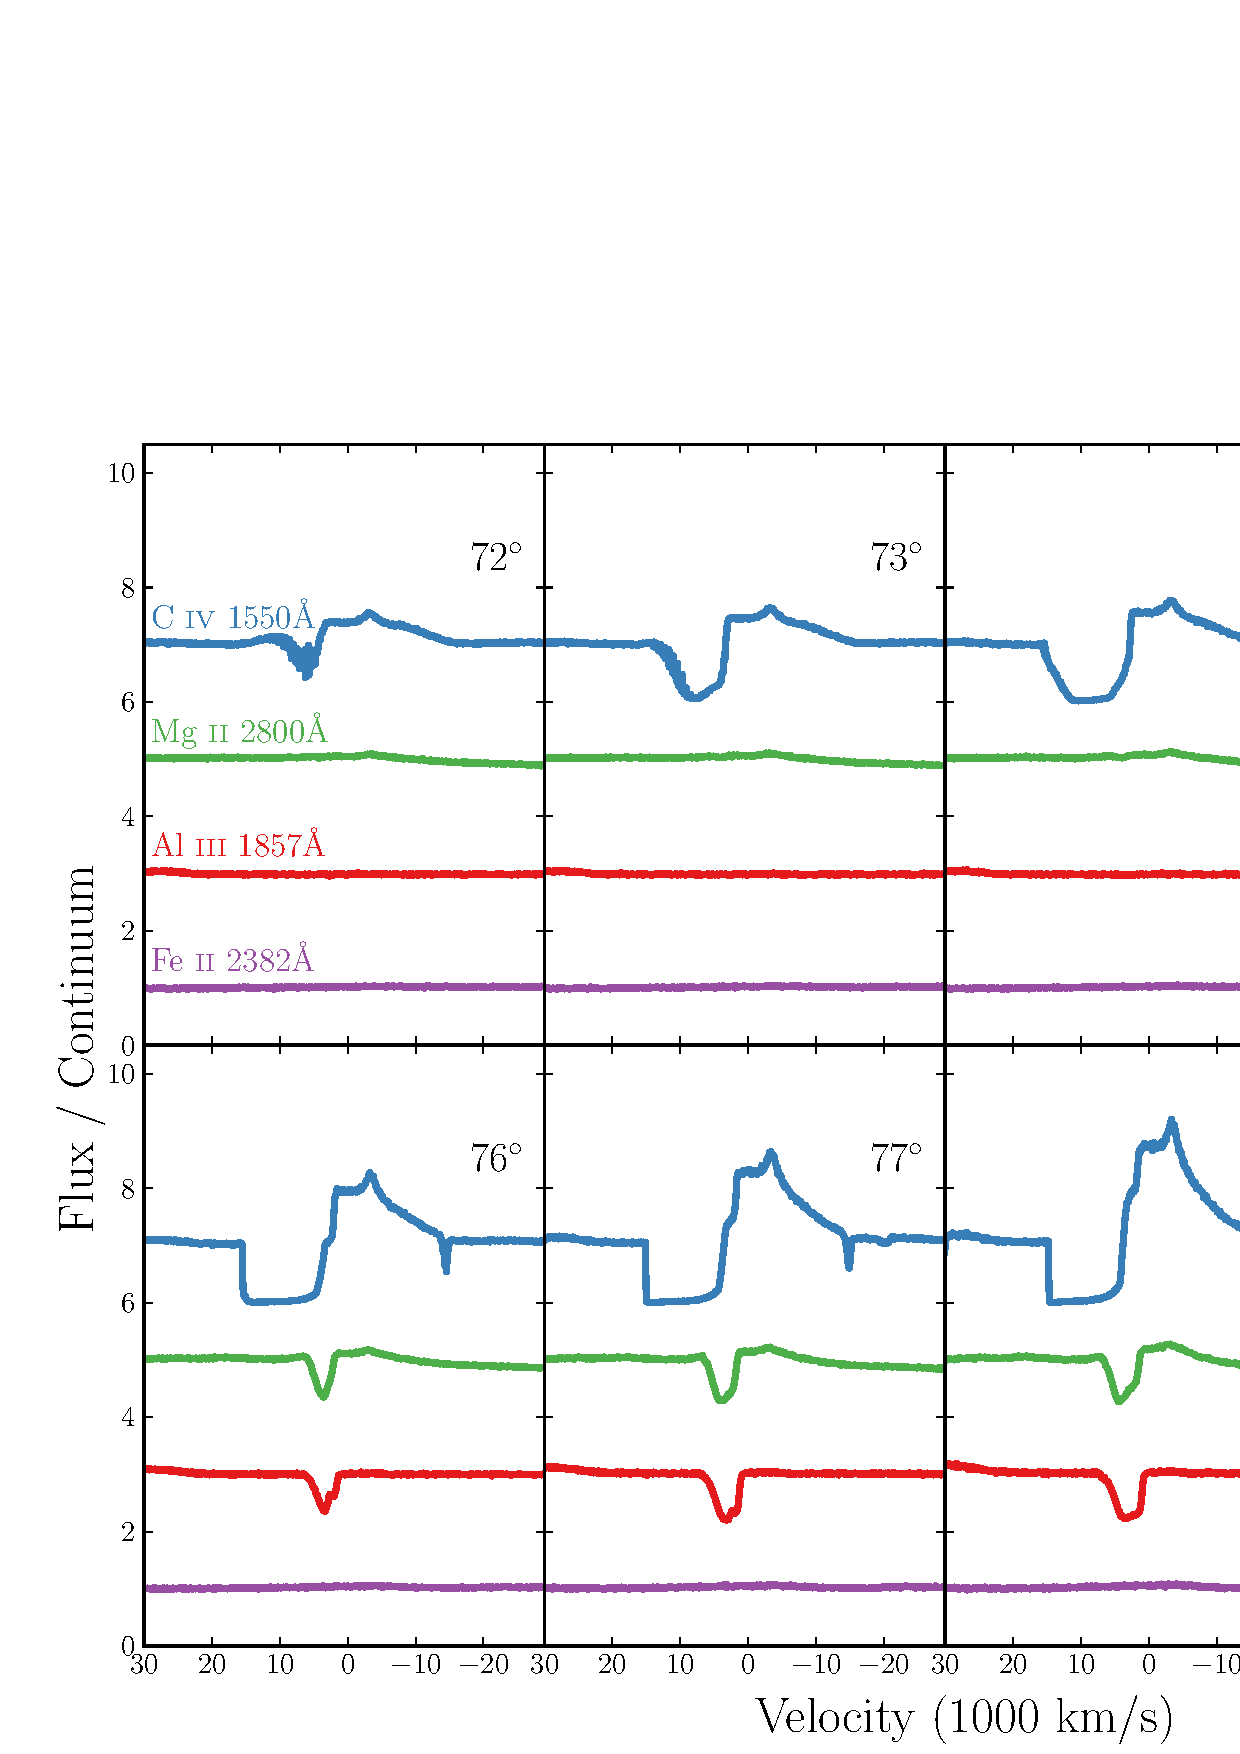
\includegraphics[width=1.0\textwidth]{figures/06-agnpaper/fig7.png}
\caption
[\civ , \mg , \al\ and Fe~\textsc{ii} line profiles for wind viewing angles.]
{
\civ , \mg , \al\ and Fe~\textsc{ii} line profiles for viewing angles
from $72-79^\circ$. The profiles are plotted relative to the local
continuum with an offset applied for clarity. Lower ionization
profiles appear at a subset of high inclinations, compared
to the ubiquitous \civ\ profile.
}
\label{fig:lobal}
\end{figure*}


At high inclinations, the synthetic spectra exhibit 
blue-shifted BALs in \al\ and \mg --
the absorption lines seen in LoBALQSOs -- 
and even show absorption in Fe~\textsc{ii}
at the highest inclinations. Line profiles in velocity space 
for \civ, \al\ and \mg, are shown in Fig.~\ref{fig:lobal} for a range
of BALQSO viewing angles. Ionization stratification
of the wind causes lower ionization material to have a 
smaller covering factor, 
as demonstrated by figures~\ref{fig:wind} and \ref{fig:lobal}.
This confirms the behaviour expected from a unification model such as Elvis (2000). 
LoBALs are only present at viewing angles close to edge-on ($i>75^\circ$),
as predicted by polarisation results \citep{brotherton1997}.
As observed in a BALQSO sample by \cite{filizak2014}, 
the model BAL troughs are wider and deeper when low ionization 
absorption features are present,
and high ionization lines have higher blue-edge velocities than the 
low ionization species.
There is also a correlation between the strength of LoBAL features
and the amount of continuum attenuation at that sightline, particularly
blueward of the Lyman edge as the low ionization base 
intersects the line-of-sight. 
A model such as this therefore predicts that LoBALQSOs and FeLoBALQSOs 
have stronger Lyman edge absorption and 
are more Compton-thick than HiBALQSOs and Type 1 quasars.
An edge-on scenario also offers a potential explanation for the rarity of LoBAL and
FeLoBAL quasars, due to a foreshortened and attenuated continuum, 
although BAL fraction inferences are fraught with complex selection 
effects \citep{goodrich1997,krolikvoit1998}.


\section{Discussion}
\label{sec:qso_discuss}

\subsection{Parameter Sensitivity}
\label{sec:param_sens}

\begin{figure*}
\centering
\includegraphics[width=0.8\textwidth]
{figures/06-agnpaper/thesis_c4_grid.png}
\caption
[Equivalent widths and BALnicities of some important lines for the quasar wind grid.]
{
The EW of the \civ~$1550$~\AA\ line at $20^\circ$ plotted against a) the 
$BI$ of \civ~$1550$~\AA\ at $75^\circ$, b) the EW of the \mg~$2800$~\AA\ line 
at $20^\circ$ and c) the EW of \la\ at $20^\circ$. The circles correspond 
to the simulation grid for two different values of $f_V$, and the fiducial 
model is marked with an orange star. 
I also show a higher X-ray luminosity model and a higher mass loss rate
with a red star.
}
\label{fig:grid}
\end{figure*}

Having selected an individual fiducial model from the simulation grid, it is important
to briefly explore how specialised this model is, and how small parameter
changes can affect the synthetic spectra. Fig.~\ref{fig:grid}
shows the EW of \la, \civline\ and \mgline\ 
for a representative low inclination, and the $BI$ for a 
representative high inclination, as produced by the models in the simulation
grid. A few conclusions can be drawn from this plot straight away. 
First, almost all the models with 
$f_V=0.1$ are over-ionized and 
fail to produce strong \civ\ BALs or emission lines. Second,  
it is difficult to significantly increase line emission while
keeping the luminosity and mass-loss rate of the system fixed. 
I show an additional point on Fig.~\ref{fig:grid} corresponding to a 
model with an order of
magnitude higher X-ray luminosity and double the mass loss rate. As expected, 
this results in far higher line EWs, but fails to produce BALs, because
the collisionally excited emission swamps the BAL profile. In addition,
this model would lie well above the expected $L_{2kev}-L_{2500}$ 
relation in Fig.~\ref{fig:xray}. Such a high X-ray luminosity could therefore 
not be the cause of the strong line emission seen in {\em all} Type 1 quasars.

The parameter search presented here is by no means exhaustive, and
conclusions may be limited by the specific parameterisation of the outflow 
kinematics used. Nevertheless, I suggest that the angular distribution
of both the line and continuum emission is perhaps the crucial 
aspect to understand. With this in mind, obtaining reliable orientation 
indicators appears to be a crucial observational task if we are to
further our understanding of BAL outflows and their connection, or lack thereof, to the 
broad line region. 

\subsection{Inclination Trends: FWHM and EW}
\label{sec:ew_in_model}

Broad line EWs increase with inclination in the fiducial model.
This trend means that even though models with
significantly denser and more strongly irradiated winds
can match the line EWs fairly well at low inclinations, they also
produce overly strong red wings to the BAL P-Cygni profiles at high inclinations.
This trend with inclination is directly related to limb-darkening 
and foreshortening of the model continuum. 
However, it appears to contradict observations, which show remarkably uniform emission
line properties in quasars and BALQSOs \citep{weymann1991,dipompeo2012b}. 

In order to quantitatively assess how emission lines change with 
inclination when blue-shifted absorption 
may affect the line profile, I define the `red wing equivalent width' (EW$_{RW}$) as
\begin{equation}
\mathrm{EW}_{RW} = \int_{\lambda_0}^{\lambda^\prime} \left( 1 - \frac{F_\lambda}{F_0} \right) d\lambda,
\label{rwew}
\end{equation}
where $F_0$ is the continuum flux, and the integral is calculated from $\lambda_0$, line centre,
to a wavelength $\lambda^\prime$ where the flux has returned to the continuum level.
This quantity is shown as a function of inclination in Fig.~\ref{fig:ew_in_model} for the \civ\ UV line.
I also show $1/2$ the EW value, together with the standard deviation, from \cite{dipompeo2012b}.

\begin{figure*}
\centering
\includegraphics[width=0.8\textwidth]{figures/ewpaper/ew.png}
\caption
[EW$_{RW}$ as a function of inclination in the fiducial model.]
{
EW$_{RW}$ as a function of inclination in the fiducial model, compared
to 1/2 EW from the quasar sample of Di Pompeo et al. (2012; D12). The shaded region
corresponds to the standard deviation of the D12 sample.
}
\label{fig:ew_in_model}
\end{figure*}

The variation of EW with inclination is significantly 
larger than the variation across the quasar population.
The angular distribution of the disc 
continuum and line emission is clearly crucially important in 
determining the emergent broad line EWs, as suggested by, e.g., 
the analysis of \cite{risaliti2011}. 
I shall explore this question further in chapter 6.  

\subsubsection{FWHM and Black Hole Mass Estimates}

In a recent study, \cite[hereafter Y16]{yong2016} used the SV93 wind prescription to
assess the variation of full-width at half-maximum (FWHM) of 
\hb\ (and resultant BH mass estimates)
with inclination in a disc wind model. 
Although their model is fairly simple -- 
it does not include, for example, full radiative transfer or ionization physics --
this analysis still gives interesting insights into how emission lines
from a disc wind might bias BH mass estimates.

If the BLR gas is virialised, as often assumed, then the black hole mass
is related to the velocity dispersion, $\Delta v$, of the gas by
\begin{equation}
M_{BH} = f \frac{\Delta v^2 R_{BLR}}{G},
\end{equation}
where $R_{BLR}$ is some appropriate emissivity-weighted radius and is often 
either assumed, estimated from ionization arguments or calculated from reverberation
mapping. When using the FWHM of a broad emission line to estimate the velocity disperson the above
equation can be rewritten as
\begin{equation}
M_{BH} = f_{FWHM}~\left[c~\frac{(FWHM)}{\lambda_0}\right]^2~\frac{R_{BLR}}{G},
\end{equation}
where $\lambda_0$ is the central wavelength of the line in question
and the FWHM is in the same wavelength units.

In our benchmark disc wind model, the BH mass is known, and determines
the escape velocities and rotational motions of the outflow. Thus, 
using a typical radius for line formation in the model, it is trivial to 
estimate $f_{FWHM}$ for each viewing angle. Fig.~\ref{fig:FWHM}
shows $f_{FWHM}$ as a function of inclination for the 
\ha\ emission line in the fiducial model, assuming $R_{BLR}=10^{17}$~cm. 
The results are compared to predicted values for five Seyfert I galaxies
from dynamical modelling \citep[][hereafter P14]{pancoast2014b}, 
and the Y16 predictions. Y16 designed two models 
in order to mimic those proposed by MCGV95 and \cite{elvis2000}, 
whose models are described in section~\ref{sec:wind_models}. 
Note that I have used FWHM of \ha\ rather than \hb\ due to the
low \hb\ luminosity at some viewing angles. Nevertheless,
this value should trace $f_{FWHM}$ from \hb\ fairly well.

\begin{figure}
\centering
\includegraphics[width=0.8\textwidth]{figures/06-agnpaper/f_factor.png}
\caption
[$f_{FWHM}$ as a function of inclination from the fiducial model.]
{
$f_{FWHM}$ as a function of inclination from the fiducial model
for three different lines. The Yong et al. (2016) 
predictions from two models, and the Pancoast et al. (2014) modelling results
for five Seyfert I galaxies are also shown.
}
\label{fig:FWHM}
\end{figure}

At `quasar-like' angles ($0^\circ-60^\circ$), the values from the model presented here 
agree fairly well with the predictions
of Y16 from their simpler analysis, suggesting that,
at least in this specific set-up, 
radiative transfer and ionization has a minimal role in determining
the emergent FWHM at those angles. Instead, at low inclinations 
the effect is dominated by velocity projection
effects. At inclinations looking into the wind radiative transfer
and shielding effects become important, and the FWHM can actually
decrease. The similarity in the shape of the curve to the P14 results suggest 
that the behaviour of FWHM is somewhat degenerate with the BLR
geometry. P14 found a thick disc model for the BLR best reproduced
the observations, but these results suggest that a wind model can mimic 
the behaviour of a disc-shaped BLR. Overall, the strong inclination dependence
of $f_{FWHM}$ strengthens the argument that viewing angle can introduce
significant uncertainty into virial mass estimates, and that individual
values for $f_{FWHM}$ should really be used for different objects
\citep[e.g.][]{decarli2008,kollatschny2011,pancoast2014a,pancoast2014b,shenho2014,brotherton2015,yong2016}.
% The reason for the significantly lower values for \mgii\ is that
% it is actually formed well inside $R_{BLR}=10^{17}$~cm, highlighting
% the dangers of using a single BLR radius for BH mass estimates
% from different lines.


%%%%%%%%%%%%%%%%%%%%%%%%%%%%%%%%%%%%%%%%%%%%%%%%%

% SUMMARY

%%%%%%%%%%%%%%%%%%%%%%%%%%%%%%%%%%%%%%%%%%%%%%%%%

\section{Summary And Conclusions}
\label{sec:qso_conclusions}
I have carried out MCRT simulations using a simple
prescription for a biconical disc wind, with
the aim of expanding on the work of H13. To do this, two main
improvements were necessary: First, I included a simple treatment of 
clumping, and second, 
the modelling of recombination lines was improved by treating H and He as
`macro-atoms'. 
Having selected a fiducial model from an initial simulation grid,
I assessed the viability of such a model for geometric 
unification of quasars, and found the following main points:
\begin{enumerate}
\item Clumping moderates the ionization state
sufficiently to allow for the 
formation of strong UV BALs while agreeing well with the X-ray
properties of luminous AGN and quasars. 
\smallskip
\item A clumpy outflow model naturally 
reproduces the range of ionization states
expected in quasars, due to its stratified density
and temperature structure. 
LoBAL line profiles are seen at a subset of viewing angles, and Fe~\textsc{ii}
absorption is seen at particularly high inclinations. 
\smallskip
\item The synthetic spectra show \la\ line and weak He~\textsc{ii}~$1640$~\AA\ line
as a result of the improved treatment of recombination using macro-atoms. 
Balmer emission lines and a Balmer recombination continuum are also
seen in the optical spectrum, but this
is only really significant at high inclination where 
the continuum is suppressed.  
\smallskip
\item The higher X-ray luminosity causes a significant 
increase in the strength of the collisionally excited emission
lines produced by the model. 
However, the equivalent-width ratios of the emission lines do not match
observations, suggesting that a greater volume of dense ($n_e\sim10^{10}$~cm$^{-3}$)
material may be required.
\smallskip
\item The line EWs in the synthetic spectra increase with inclination.
BAL and non-BAL quasar composites have comparable EWs, so the fiducial model
fails to reproduce this behaviour.
 If the BLR emits fairly isotropically then for a 
foreshortened, limb-darkened accretion disc 
it is not possible to achieve line ratios at low inclinations 
that are comparable to those at high inclinations. 
I suggest that understanding the angular distribution of 
line and continuum emission is a crucial question for theoretical models.
\smallskip
\item There is also a strong dependence on inclination in the FWHM of
\ha, as found in numerous other studies. The results add to the growing evidence
that inclination introduces large uncertainties into virial 
BH mass estimates, and suggest that disc wind models might produce similar inclination-dependent
behaviour in $f_{FWHM}$ to disc-shaped BLR models.
% Furthermore, this is conclusion is independent of the assumed 
% BLR geometry and size.
\end{enumerate}
This work confirms a number of expected outcomes from a geometric unification 
model, and suggests that a simple biconical geometry such as this can come close to 
explaining much of the  phenomenology of quasars. However, these conclusions pose 
some challenges to a picture in which BALQSOs are
explained by an {\em equatorial} wind rising from a classical thin disc, and suggest 
the angular distribution of emission is important to understand if this 
geometry is to be refuted or confirmed. I suggest that obtaining reliable 
observational orientation indicators and 
exploring a wider parameter space of outflow geometries in simulations
are obvious avenues for future work. % Experiment 2

\newpage
\lhead{\emph{6. Quasar Emission Lines as Probes of Orientation and Unification}}
\chapter{Quasar Emission Lines as Probes of Orientation and Unification}



{\em This chapter is based on a paper in prepation:

Matthews J. H., Knigge C., 
`Quasar Emission Lines as Probes of Orientation and Unification',
to be submitted to MNRAS.}


%%%%%%%%%%%%%%%%%%%%%%%%%%%%%%%%%%%%%%
%
%          ABSTRACT
%
%%%%%%%%%%%%%%%%%%%%%%%%%%%%%%%%%%%%%%%
\maketitle

\section{Introduction}

In the previous chapter, I presented tests of geometric unification
models using MCRT and photoionization simulations. 
One of the key results from that analysis is that trends with
inclination prohibit models with equatorial outflows matching
observations, as the EW of the emission lines tend
to increase with inclination. This trend has clear implications for
the geometries of BAL outflows; the viewing angle may determine many
of the selection effects at work and must therefore be understood
before the true covering factor of BAL outflows can be accurately 
determined. The covering factor and opening angle of the outflow
are important quantities to measure in order to calculate the
feedback efficiency \citep[e.g.][]{borguet2012}, 
and understand the outflow physics \citep[e.g.][]{proga2005}. 

Unlike in galactic accretion disc systems, measuring inclinations
for quasars and AGN is notoriously difficult, and obtaining 
reliable orientation indicators is thus an important observational
goal for the community. Perhaps as a result of this problem, 
directly opposing geometries have been proposed for 
BAL outflows (see section~??). Here, I use observational 
data from the Sloan Digital Sky Survey to constrain the inclinations
of BAL quasars. Similar attempts have been made previously with
different diagnostics; for example, by considering 
radio measurements \citep{zhou2006,dipompeo2012a}, 
polarisation \citep{brotherton2006}
and emission line properties \citep{dipompeo2012b}.  

This chapter is structured as follows. First, I describe
the data sample and selection criteria being used. I begin by
simply examining the distributions of the EW of the \oiiifull\ emission line,
\ewo, and comparing the BAL and non-BAL quasar distributions. 
In section~\ref{sec:disc_agn} I review the angular distribution of 
continuum emission one would expect from simple $\alpha$-disc models, 
as well as exploring more advanced disc models computed
with \agn. I then use these theoretical 
angular distributions applied to a simple toy model in 
section~\ref{sec:mc_angular},
and conduct MC simulations in an attempt to fit the observed LoBAL and non-BAL
quasar distributions of \ewo, using a similar approach to 
\cite{risaliti2011}. I also discuss the broad emission
line distribution in HiBAL quasars more detail in this section. 
In section~\ref{sec:discuss_ew} I discuss the results
in the context of radio and polarisation measurements of AGN, as well
as exploring the location of BAL quasars in `Eigenvector 1' parameter space.
Finally, in section~\ref{sec:ew_conclusions}, I summarise the results.

% {\bf{\sl{\huge Abstract}}}

% The incidence of broad absorption lines (BALs) in quasar samples is 
% often explained by a geometric unification model consisting
% of an accretion disc and an associated outflow.
% This outflows is assumed to have a covering factor roughly equivalent to
% the BAL fraction, $f_{BAL}$. We test this model
% by examining ultraviolet (UV) emission line equivalent-widths. 
% We find that a model in which the 
% continuum emission arises from a geometrically thin, 
% optically thick accretion disc is inconsistent with this property
% unless (i) the line emission has the same angular distribution of 
% emission as the continuum or (ii) BAL quasars are viewed from a low or intermediate inclination. 
% We examine whether an accretion disc can emit isotropically, and
% demonstrate that general relativistic effects cannot sufficiently isotropise the 
% radiation field in the UV. 
% We suggest that reprocessing by outflows, or limb brightening due to X-ray irradiation, may play a role.
% We then explore in what limits line emission can emit with the same angular
% distribution as a foreshortened, limb-darkened disc, and discuss our results
% in the context of other observational studies of broad emission line 
% equivalent-widths in quasars.
% Finally we explore geometries in which BAL quasars are viewed
% from a low or intermediate inclination with reference to polarisation
% and modelling results. We also discuss the effect of the outflow 
% geometry on the inferred BAL fraction. We favour a scenario in which the 
% BAL outflow is {\em not} equatorial, and BAL quasars
% are instead viewed from $\sim45^\circ$ as suggested from radio measurements,
% but a number of open questions remain.

% \clearpage

%%%%%%%%%%%%%%%%%%%%%%%%%%%%%%%%%%%%%%
%
%          INTRODUCTION
%
%%%%%%%%%%%%%%%%%%%%%%%%%%%%%%%%%%%%%%%

%{\em This chapter is based on a paper in preparation of the same title, 
%due to be submitted to MNRAS.}

%\section{Introduction}
% {\color{blue}
% Introduction to the topic, particular relating to unification
% and BAL geometries. At the moment this is a placeholder.
% }
% \bigskip

%\noindent
% A number of quasar unification schemes have attempted to explain 
% the incidence of BAL quasars in terms of an outflow which rises 
% from an accretion disc \citep[e.g.][]{MCGV95, elvis2000}. 
% The covering factor of this outflow is then
% expected to determine the BAL fraction, $f_{BAL}$, thought to be
% between $20\%$ and $40\%$ 
% \citep{weymann1991, reichard2003, knigge2008, allen2011}.
% These outflows are of wide-reaching astrophysical significance as 
% they may be an efficient way for the central accretion engine to interact
% with its galactic environment (REFs), potentially explaining 
% for the $M-\sigma$ relation (REFs).

% Unlike in galactic accretion disc systems, measuring inclinations
% for quasars and AGN is notoriously difficult, and obtaining 
% reliable orientation indicators is thus an important observational
% goal for the community. Directly opposing 
% geometries have been proposed for BAL outflows, mostly from observations
% of radio-loud sources. A number of polarisation
% studies of BALQSOs have measured large angle differences 
% from the radio jet, implying an equatorial viewing angle 
% \citep{goodrich1995, cohen1995,brotherton2006}.
% Conversely, Punsly (1991) suggests a polar geometry.
% This is supported by very high brightness temperatures 
% in some RL BALQSOs \citep{zhou2006} 
% and the fact that RL BALQSOs possess similar radio spectral 
% indices to normal RL quasars \citep{bruni2012}.  
% In addition, \cite{marin2013} find a bending angle of 
% $\sim45^\circ$ is required to 
% explain the polarisation dichotomy of type 1 and 2 AGN using an Elvis-type wind 
% model (Elvis 2000) --  a conclusion which is potentially extendable to BAL quasars.

% BALQSOs and quasars generally possess remarkably similar emission line properties 
% \citep[e.g.][]{weymann1991,reichard2003}. This, along with Occam's razor (see figure 1),
% is one of the reasons why they are thought to be drawn from the same population 
% as non-BAL quasars. In this paper, we start by verifying the uniformity 
% of emission line properties
% between BAL and non-BAL quasars. We then derive relationships for
% the expected angular distribution of emission for accretion discs 
% (section~\ref{disc}) and emission lines (section~\ref{lines}). Finally, we discuss
% these results in the context of unification models and offer 
% a number of possible scenarios.

% In the previous chapters we have explored quasar unification schemes
% in which the incidence of BAL quasars is explained in terms of an outflow which rises 
% from an accretion disc \citep[e.g.][]{MCGV95, elvis2000}. In chapter 5,
% we found that a biconical wind model can reproduce much of the qualitative 
% behaviour expected from a unified model, with some shortcomings. 
% In particular, we found an angular dependence of emission-line equivalent 
% width (EW), such that the EWs were much stronger at high inclination.
% Here, we attack the problem from a different angle (but informed by the 
% previous study), by examining UV and optical emission lines from the Sloan Digital Sky 
% Survey and the potential effects of orientation on their EW distributions.

% Unlike in galactic accretion disc systems, measuring inclinations
% for quasars and AGN is notoriously difficult, and obtaining 
% reliable orientation indicators is thus an important observational
% goal for the community. Directly opposing 
% geometries have been proposed for BAL outflows, mostly from observations
% of radio-loud sources. A number of polarisation
% studies of BALQSOs have measured large angle differences 
% from the radio jet, implying an equatorial viewing angle 
% \citep{goodrich1995, cohen1995,brotherton2006}.
% Conversely, Punsly (1991) suggests a polar geometry.
% This is supported by very high brightness temperatures 
% in some RL BALQSOs \citep{zhou2006} 
% and the fact that RL BALQSOs possess similar radio spectral 
% indices to normal RL quasars \citep{bruni2012}.  
% In addition, \cite{marin2013} find a bending angle of $\sim45^\circ$ is required to 
% explain the polarisation dichotomy of type 1 and 2 AGN using an \cite{elvis2000} wind 
% model --  a conclusion which is potentially extendable to BAL quasars.



\section{Data Sample}
% {\color{blue}
% First we need to show that emission line properties of 
% quasars and BAL quasars really are similar. Do that with histograms 
% of EWs. We will probably show a mixture of emission lines so we cover
% allowed dipole, forbidden and intercombination lines. 

% Questions:

% \begin{itemize}
% 	\item Do we need some kind of test statistic here? e.g. K-S
% 	\item Perhaps we should derive theoretical quasar distribution with different 
% 		  inclination cutoffs?
%     \item Do we want to repeat the analysis of Risaliti et al? 
%     \item It may make sense to start with theory, derive model distributions and 
%     	  then test them against real distributions for different physical models
%     	  and inclination cutoffs?
% \end{itemize}
% }
% \begin{figure*} %fullpage
% \centering
% \includegraphics[width=1.0\textwidth]{figures/ewpaper/composites.png}
% \caption
% {
% SDSS Composite spectra
% }
% \label{fig:composite}
% \end{figure*} %fullpage
% The Sloan Digital Sky Survey DR7 contains ~10,000 objects in its quasar
% catalog. Many of these have been fitted with quasar templates, allowing 
% easy comparison of the equivalent width properties between the BAL and 
% non-BAL subsamples. Figure 2 shows histograms of a number of different 
% emission line properties. As found by previous authors, we find that BAL
% and non-BAL quasars really do seem to possess very similar emission line 
% properties.

% \begin{table}
% \begin{tabular}{p{2cm}p{1cm}p{1cm}p{1cm}p{1cm}}
% Sample & Redshift Range & Number of non-BAL Objects & Number of BAL objects & Number of LoBAL objects \\
% \hline \hline 
% A & $?<z<?$ & 
% \hline 
% \end{tabular}
% \caption{
% The properties of our subsamples, built from the SDSS DR7
% quasar catalog.
% }
% \label{tab:samples}
% \end{table}

\begin{figure*} %fullpage
\centering
\includegraphics[width=1.0\textwidth]{figures/ewpaper/bals_2x2_scatter.png}
\caption
{
BH mass and Eddington fraction for the BAL samples plotted 
over the overall quasar sample from S11.
}
\label{fig:bal_scatter}
\end{figure*} %fullpage

\begin{figure*} %fullpage
\centering
\includegraphics[width=1.0\textwidth]{figures/ewpaper/ew_hist_qsos.png}
\caption
{
Histograms of equivalent widths for three emission lines from the two different samples.
}
\label{fig:ew_hists}
\end{figure*} %fullpage

The data sample is based upon the
\citet[][hereafter S11]{shen2011} catalog of
105,783 quasars from the The Sloan Digital Sky Survey (SDSS) 
Data Release 7 (DR7). 
As I will use emission line diagnostics in this study,
this sample must be further divided according to which 
emission lines are present in 
the SDSS wavelength range at a given redshift. 
Sample A contains all quasars within the redshift range $0.35<z<0.83$, 
such that the \mgline\ and \oiiifull\ line EWs are both measured, 
and \mg\ BAL identification
is possible.  Sample B contains all quasars within the redshift 
range $1.45<z<2.28$, such that 
the EWs and presence of BALs in Mg II 2800A and CIV 1550A are both measurable.
The details of these samples are shown in table 1.
The mass and Eddington fraction measurements from S11 of the two samples,
are shown in Fig.~\ref{fig:bal_scatter}
against the background distribution of all S11 quasars.

S11 are careful to take into account traditional problems with quasar line fitting,
such as narrow line or Fe pseudocontinuum contamination, in their fits to 
emission line profiles and resultant EW measurements. For \mgline\
this includes careful subtraction of the Fe emission using the \cite{vestergaard2001}
templates. This subtraction is not included for \civfull,
as the Fe emission is less prominent and harder to model. This may lead to
a systematic overestimate by $\sim0.05$ dex in the \civ\ line EW. 
The \oiiifull\ line is fitted
with a Gaussian and the flux ratio with the sister component 
of the doublet, \oiiidoublet, is found to agree well with the theoretical
expectation of around 3, implying a reliable subtraction of broad \hb.
To mask out the effects of e.g., absorption, on \civ, S11 ignore 
$3\sigma$ outliers in the fit to the profile. Based on these
considerations, the S11 catalog makes for a reliable set of EW 
measurements. This is especially true when making inferences from 
multiple emission lines, as systematics inherent to individual lines 
or spectral windows are less likely to affect the analysis as a whole.

In attempting to draw broad conclusions about unification models as a whole,
I would ideally construct a large, homogenous dataset of 
{\em HiBAL} and non-BAL quasars, both with \oiiifull\ EWs. Unfortunately,
the wavelength limits of SDSS do not allow this, and only LoBAL quasars have 
both BALs and \ewo\ measurements. One of the problems with
using just LoBAL quasars as tests of unification is that there is evidence 
that they are drawn from a different population than normal quasars, perhaps
suggesting an {\em evolutionary} origin. Examples include anomalously 
high LoBAL fractions in dust-reddened quasar samples \citep{urrutia2009} 
and infra-red selected samples \citep{dai2012}; 
although see also \cite{lazarova2012}.
% in SDSS by cross-matching the S11 catalog with BALs identified in the HST 
% COS archive.BALs were selected from the COS spectra using the balnicity index, 
% $BI$, defined in equation~??. HST objects were designated as HiBALS 
% by satisfying the condition that $BI>0$ in one of CIV, NV, SiIV.


Fig. 2 shows histograms of a number of different 
emission line properties for samples A and B. 
As discussed by previous authors \cite[e.g.][]{weymann1991}, I find that BAL
and non-BAL quasars really do seem to possess very similar emission line 
properties. The EW is related to the intrinsic, `face-on' equivalent width,
$\ew_*$ by the equation
\begin{equation}
\ew = \ew_* /\epsilon(\theta)
\end{equation}
where $\theta$ is the viewing angle with respect to the symmetry axis 
and $\epsilon(\theta)$ is the `angular emissivity function', which describes 
how the continuum luminosity from the disc varies as a function of viewing angle.
For a foreshortened disc this is simply $\epsilon(\theta) = \cos \theta$. 
Note that this assumes isotropic line emission, but the effect of line
anisotropy is discussed in section~\ref{sec:}

Thus, if BAL quasars are viewed from a larger viewing angle on average then one
would expect them to possess higher EWs, with a broader distribution.
It is already apparent from figure 1 that the BAL distribution mean 
is not significantly higher than the non-BAL
mean -- in fact, in many cases it is lower. This is not expected from a model
in which the continuum is foreshortened and BAL outflows are at all equatorial.
This problem is examined further in section~\ref{sec:mc_angular}. 
First, I will examine the motivations for different forms of \ept\ 
in AGN and quasars.

\section{The Angular Distribution of Emission from an Accretion Disc and Broad-Line Region}
\label{sec:disc_agn}

\noindent 
As introduced in chapter 1, the most widely-used theoretical model for an accretion disc
is the so-called `$\alpha$-disc' model of SS73. 
There are a number of well-documented problems when fitting 
AGN SEDs with SS73 accretion disc models (see section~\ref{sec:disc_continuum}), 
Despite these problems, \cite{capellupo2015} recently had 
some success fitting spectra of AGN when the effects of
GR, mass-loss and comptonisation were included.
In this section, I start by discussing the angular distribution of
emission from an SS73 disc, before exploring opacity and GR 
effects. In order to do so, I use \agn\
\citep{hubeny2000,davishubeny2006,davis2007}. I stress that the 
discussion here is not limited to SS73 discs; the only real condition
for the angular distributions derived here is that the 
disc is geometrically thin and optically thick.

\subsection{Standard Thin Disc Models}

\noindent
Any geometrically thin, optically thick disc will appear
foreshortened and limb darkened (if temperature decreases
with height from the central disc plane). 
Foreshortening is a simple $\cos \theta$ geometric effect, 
where $\theta$ is the inclination with respect to the vertical z axis, which
is perpendicular to the disc plane.
Limb darkening, $\eta(\theta)$, is given by
\begin{equation}
\eta(\theta) = a \left( 1 + b \cos \theta \right),
\end{equation}
where $a$ is a normalisation constant and $b$ governs the strength
of the limb darkening. $b=3/2$, known as the Eddington approximation
tends to given good agreement with solar observations 
\citep[e.g.][]{mihalas}. The two effects can be 
combined to give an angular emissivity function, of
\begin{equation}
\epsilon(\theta) = a \cos \theta \left( 1 + \frac{3}{2} \cos \theta \right).
\end{equation}

\subsection{Including GR and Opacity Effects}

\begin{figure}
\centering
\includegraphics[width=1.0\textwidth]{figures/ewpaper/agnspec.png}
\caption
{
Monochromatic continuum luminosities from AGNSPEC and classical thin disc
models.
}
\label{fig:agnspec_disc}
\end{figure} 


\noindent
In reality, limb darkening is not frequency independent and 
depends on the bound-free and bound-bound opacities in the disc.
In addition, it has been shown that GR can `isotropize' the radiation
field in XRBs \citep{zhang1997,munozdarias2013}, in some cases overcoming
foreshortening effects. To assess the impact of GR and disc opacities
on \ept, I use \agn\ models, which conducts a stellar atmosphere calculation
to obtain the SED from a series of annuli, before using the \kerrtrans\ code 
to calculate the emergent SED by ray-tracing along Kerr geodesics.
Fig.~\ref{fig:agnspec_disc} shows \ept\ as a function of 
$\theta$ for \agn\ models for minimally and maximally spinning BHs,
compared to foreshortened and limb-darkened predictions for SS73 models.
Although the continuum is significantly more isotropic at $500$\AA,
there is very little effect redward of around $1000$\AA, which is the relevant
region of \ept\ for \oiiifull, \civline\ and \mgline . 
In fact, using the foreshortened estimate is 
the conservative approach in these regimes. I will thus adopt \ept$=\cos \theta$
for the remainder of this work.


% Including GR, Comptonisation and Opacity Effects

% \subsection{Alternative Continuum Models: Irradiation and Truncated Discs}

% Alternative Models exist...


% \subsection{Angular Distribution of Line Emission}

% Lines can be classified according to whether they violate quantum selection rules.
% In order of decreasing oscillator strength, they comprise
% dipole permitted transitions, such as \civline\ and \hb, 
% semi-forbidden or intercombination
% lines such as \ciiiline, and forbidden lines such as \oiiifull.
% As the optical depth in a line is proportional to the oscillator strength,
% we can see that we should expect lines such as \oiiifull\ to be optically
% thin, whereas dipole transitions may be subject to local line
% opacity effects. It is worth noting, of course, that all lines can be absorbed by 
% continuum processes. Ignoring the effect of obscuration, we thus expect all 
% forbidden lines to be isotropic (i.e. \eptl$={\rm constant}$. 
% But what about permitted lines? What is their expected angular distribution
% of emission





\section{Predicted EW Distributions Compared to Observations}
\label{sec:mc_angular}

\subsection{Fitting the Quasar Distribution}
\label{sec:fitting}

\citet[][hereafter R11]{risaliti2011} analysed the \ewo\ 
distribution of 6029 quasars in SDSS DR5. They demonstrated
that a foreshortened disc and isotropic \oiiifull\ line produces
a high EW tail to the distribution with a characteristic 
slope of $\Gamma_{EW}=-3.5$. In order to first reproduce their
result and discuss its implications, I have 
created a sample according to their selection
criteria. The criteria are that the object in question lies in the redshift
range 0.01 to 0.8, have an absolute magnitude $M_i>22$, an 
apparent magnitude $m_i>19.1$, and signal to noise per pixel of greater
than 5. Using the updated SDSS quasar sample of S11, this defines
a sample of 14,424 quasars.

To fit the distribution, I conduct the following procedure,
which is similar to the method R11 use to demonstrate that the power
law tail is expected.
\begin{enumerate}
	\setlength\itemsep{1em}
	\item A set of isotropic angles is chosen such that 
	$P(\theta)\propto d\Omega(\theta)$. 
	If $\theta<\theta_{1}$ then the fake object is designated as unobscured, 
	and otherwise the object is ignored. 
	\item To be included in the sample, the object also has to 
	survive a selection test
	to simulate the distribution of angles in a flux-limited sample.
	This is done by drawing a random sample from the real quasar sample, 
	and calculating a `doubly observed continuum flux', $F_O$ at $5100\AA$ 
	(rest frame), such that $F_O = F_{5100}~\epsilon(\theta)$. The flux limit
	is set at $5\times10^{-13}$~erg~s$^{-1}$~cm$^{-1}$~\AA$^{-1}$, but the results
	are fairly insensitive to the limit chosen.
	\item For each mock sample, an EW$_*$ is drawn from an intrinsic 
	(i.e. `face-on') EW distribution for quasars. This is assumed to be a
	gaussian. The mean, $\mu_*$, and width, $\sigma_*$, of this Gaussian
	can either be set arbitrarily -- for example, to demonstrate trends
	in mock data -- or obtained from a $\chi^2$ fit to the observed EW
	distribution.
	\item A mock EW is estimated such that $\ew = \ew_* / \epsilon(\theta)$,
	and this process is repeated to build up a mock sample of $10^6$ objects.
\end{enumerate}
The result of this numerical experiment is, as found by R11, a distribution
with a high EW tail of slope $-3.5$. I can now vary the maximum angle, $\theta_1$,
and examine how this tail changes. Mock data for a series
of maximum angles is shown in Fig.~\ref{fig:cutoff}, for two different intrinsic 
Gaussians. The power law behaviour is only seen when the maximum angle is
sufficiently large, and a rapid decay in the distribution is observed
at a characteristic EW related to both the width and mean of the
intrinsic distribution as well as the cosine of the maximum angle.
The top panel has $\mu_*$ and $\sigma_*$ of the R11 Model 1, 
whereas the bottom panel shows a narrower distribution to illustrate the 
earlier onset of the high EW cutoff. In principle, this cutoff could
be used to infer information about the viewing angle distribution
of quasars.

\begin{figure}
\centering
\includegraphics[width=1.0\textwidth]{figures/ewpaper/cutoff.png}
\caption
{
Theoretical EW distributions from the numerical experiment 
described in section~\ref{sec:fitting} for a few different 
maximum angles. The results in the top panel use the same intrinsic
distribution as Model 1 from R11 (shown in black), 
whereas the bottom panel shows the distributions 
obtained from a narrower intrinsic Gaussian. By the time the maximum
angle is limited to around $70^\circ$ the cutoff is
clear even at moderate values of EW.
}
\label{fig:cutoff}
\end{figure}

Fig.~\ref{fig:chi2} shows the result of a $\chi^2$ minimization fit 
to the R11 sample. The best fit is achieved with a maximum angle of 
$\theta_{1}=84^\circ$ and a narrower intrinsic distribution
than model 1 of R11. The run of reduced $\chi^2$ with maximum angle
is shown in Fig.~\ref{fig:chi2_curve}, where the choice for $\mu_*$
and $\sigma_*$ is left free in each case. 
Maximum angles below $\sim80^\circ$ are strongly disfavoured
by this model. I adopt linear binning to facilitate easy comparison 
with R11, and only fit up $\ew=100$\AA\
due to poor statistics above that limit. Unfortunately, this 
makes inferring any information about a potential high EW cutoff 
difficult as a more complete sample at high EW is required. 

\begin{figure}
\centering
\includegraphics[width=1.0\textwidth]{figures/ewpaper/log_quasar_fit.png}
\caption
{
The EW distribution of quasars in the R11 sample (red errorbars)
and the best fit model with a maximum viewing angle of
$84^\circ$.
}
\label{fig:chi2}
\end{figure}

\begin{figure}
\centering
\includegraphics[width=0.8\textwidth]{figures/ewpaper/chi2_o3.png}
\caption
{
$\chi^2/dof$ as a function of maximum angle, $\theta_1$, calculated in
steps of $0.1^\circ$. The choice for $\mu_*$ and $\sigma_*$ is 
left free in each case.
}
\label{fig:chi2_curve}
\end{figure}

\subsection{Comparing non-BAL and LoBAL Distributions: Sample A}
\label{sec:bal_v_nonbal}

\begin{figure}
\centering
\includegraphics[width=0.8\textwidth]{figures/ewpaper/fig2_cartoon.png}
\caption
{
The geometry of the toy model used to carry out the Monte Carlo simulations
}
\label{fig:cartoon}
\end{figure}

% For LoBALs, \ewo\ measurements are available. This means the 
% non-BAL quasar \ewo\ distribution can actually be fitted in
% the LoBAL redshift range, and the expected LoBAL \ewo\ distribution
% predicted for a grid of $\theta_{min}$ and $\theta_{max}$. To do this,
% the procedure used to generate

In order to compare the observed distributions to those expected for LoBALs and
non-BALs I conduct a Monte Carlo simulation similar to
the process described in section~\ref{sec:fitting}, but with a few 
key differences. I once again assume $\epsilon(\theta) = \cos \theta$.
The geometry of the toy model used in this simulation is shown in
Fig.~\ref{fig:cartoon}.

First, A set of isotropic angles is generated.
If $\theta_{min}<\theta<\theta_{max}$ then the fake object 
is flagged as a mock BAL. If $\theta<\theta_{min}$ then the 
fake object is designated a non-BAL, and otherwise
the object is ignored. Once again, the object also has to 
survive a selection test based on a arbitrary flux selection limit.
I then fit the non-BAL distribution using the method described previously.
For each mock sample, a EW$_*$ is drawn from the intrinsic gaussian,
and a mock EW is estimated such that $\ew = EW_* / \epsilon(\theta)$.
This process is repeated to build up a mock sample of objects, and 
carried out for a series of pairs of $\theta_{min}$ and $\theta_{max}$.
This allows theoretical distributions for BAL and non-BAL quasars
for a series of different outflow geometries to be derived.

The diagnostics recorded from the simulation are the following four
quantities:
\begin{itemize}
	\item The $p$-value associated with the Kolgomorov-Smirnov (K-S) 
	test statistic, $p_{KS}$, in which the mock BAL sample is compared
	to the real LoBAL sample.
	\item The BAL fraction, $f_{BAL}$, is calculated from the 
	number of objects in the mock sample with $\theta_{min}<\theta<\theta_{max}$.
	\item The $\chi^2/dof$ from the fit to the non-BAL quasar distribution.
	\item $\Delta \mu$, the difference between the mean value of the mock BAL
	distribution and the mean value of the mock non-BAL distribution.
\end{itemize}
The simulation results are shown in figure~\ref{fig:contour}, in which the 
four diagnostics are plotted as a function of $\theta_{min}$ 
and $\theta_{max}$. 

As expected, equatorial viewing angles for LoBAL quasars 
are disfavoured, and furthermore, it is only possible to fit
the tail to the \ewo\ distribution if non-BAL quasars are allowed 
to be viewed from high inclinations. There is no region of parameter
space where a satisfactory fit is obtained to the quasar distribution
without simultaneously obtaining a large value of $\Delta \mu$. The
K-S test allows us to reject the null hypothesis
The simulations favour a geometry in which BAL quasars are viewed
from very similar angles to non-BAL quasars.

The conclusions here are limited by the lack of knowledge about the 
intrinsic face-on distribution of \ewo, or equivalently,
the orientations of the quasars themselves. If either of these
quantities were known then the results of the
K-S test and $\chi^2$ minimization could be used
to place more robust constraints on BAL and non-BAL viewing angles 
and the associated covering factor of the outflow.
Furthermore, the distribution of \civ\ quasar EW cannot be fit by 
the same model as the \ewo\ distribution.
% Despite these difficulties, it is still relatively easy to 
% demonstrate that the EW distribution in BAL quasars is not well produced by a 
% model in which the accretion disc is foreshortened 
% and BAL quasars are viewed from high inclinations. I will show this byconducting
% a slightly simpler Monte Carlo experiment to ascertain which geometries 
% best reproduce the observed distributions.

% First, I find that the quasar EW distribution
% cannot be well-fitted unless quasars are viewed from a wide range of angles,
% right up to edge-on. This was already known from the analysis in 
% section~\ref{sec:fitting}. However, now we can see that this region of
% parameter space is the region most disfavoured when comparing the mock BAL
% dataset to the observed BAL dataset, and outflows occupying those
% opening angles would have significantly higher EWs than the non-BAL
% quasars.

% Although the quasar EW distribution can be fitted with the above 
% model, neither the true distribution of viewing angles 
% or the intrinsic `face-on' EW distribution of the emission line in 
% question is known. If an intrinsic, face-on distribution could be constructed
% then the Kologomorov-Smirnov test and $\chi^2$ minimization could be used
% to place constraints placed on BAL and non-BAL viewing angles.
% Furthermore, the distribution of \civ\ quasar EW cannot be fit by the same
% model as the \ewo\ distribution.
% Despite these difficulties, it is still relatively easy to 
% demonstrate that the EW distribution in BAL quasars is not well produced by a 
% model in which the accretion disc is foreshortened 
% and BAL quasars are viewed from high inclinations. I will show this byconducting
% a slightly simpler
% Monte Carlo experiment to ascertain which geometries best reproduce the observed
% distributions. Throughout these simulations, 

\begin{figure*} %fullpage
\centering
\includegraphics[width=1.0\textwidth]{figures/ewpaper/mesh4_ew_o3_max_sdss.png}
\caption
{
Heat map showing the results of the MC simulation described in 
section~\ref{sec:bal_v_nonbal}. The quantities shown are discussed 
further in the text, but correspond to (clockwise from top left):
the $p_{KS}$ value from a comparison between the mock BAL dataset
and the observed BAL dataset, the reduced $\chi^2$ from the fit to
the non-BAL EW distribution, the difference in mean EW between the 
mock BAL and mock non-BAL datasets, and the BAL fraction expected
for the geometry in question.
}
\label{fig:contour}
\end{figure*} %fullpage

An additional limitation is due to the SDSS wavelength coverage
and means that only LoBALs can be used when \ewo\ is present (sample A).
I would suggest that future observational programs might 
look to build up a large sample of \ewo\ measurements for HiBAL
quasars. In the mean time, I will turn to the UV broad emission
lines to examine if the above conclusions also hold
when examining the properties of the HiBAL quasars in sample B.

\subsection{Broad Emission Lines in HiBAL quasars: Theoretical EW Distributions for Sample B}
\label{sec:hibal_v_nonbal}

\begin{figure} %fullpage
\centering
\includegraphics[width=1.0\textwidth]{figures/ewpaper/faceon_ew_c4_faceon_sdss.png}
\caption
{
Heat map showing the results of the MC simulation described in 
section~\ref{sec:hibal_v_nonbal}. The top panel shows the expected 
BAL fraction for the geometry in question, and the 
}
\label{fig:c4_faceon}
\end{figure} %fullpage

Unfortunately, due to the wavelength ocverage of SDSS, objects in 
which \civ\ BALs can be identified cannot also have measurements of \ewo. 
Furthermore, it is not possible to find a good fit to 
the non-BAL quasar \civline\ EW distribution using the method used until
now, due to the fundamentally different shape of the \civ\ line compared to
\oiii. This difference in shape could be due to line opacity effects 
(see section~\ref{sec:line_aniso}) or obscuration of the BLR, which is significantly
more compact than the NLR (see section~\ref{sec:obscure}).
Thus, to explore which geometries are favoured by the \civ\ distribution,
I conduct a simpler test, in which I make the assumption that the intrinsic
distribution is roughly equivalent to the non-BAL quasar distribution.
I repeat the procedure from the previous section, but instead draw $EW_*$
from the non-BAL quasar distribution. As I result, I only record $\Delta \mu_{EW}$
and $f_{BAL}$ as diagnostics. 

The results are shown in Fig.~\ref{fig:c4_faceon}. 
Similar trends are observed to those seen in LoBALs -- geometries
in which BAL outflows emerge at extreme inclinations should produce
dramatically higher mean values for the EW, which are not observed in 
the data. Although this analysis makes more assumptions than for the \ewo\
fitting, it still implies that BALQSOs are not viewed from significantly 
higher inclinations than non-BAL quasars.


\section{Discussion}
\label{sec:discuss_ew}
I have demonstrated that the EW distributions of the 
\oiiifull\ emission line in quasars is not consistent with a 
model in which BAL quasars are viewed from equatorial angles 
and the continuum emission originates from
a foreshortened accretion disc. This conclusion would be strengthened were 
I to include limb darkening. This conclusion is extendible to the broad 
emission lines, with the caveat that those lines are dipole 
transitions and so opacity effects can change the angular distribution of 
emission. I will now explore how the above results compare to other
observations of quasars that are expected to probe system orientation, as 
well as the potential impact of obscuration on the results.

\subsection{Eigenvector 1}

% \begin{table}
% \centering
% \begin{tabular}{p{2cm}p{2cm}p{2cm}p{2cm}}
% \hline Par. A & Par. B & $r_{corr,AB}$ (non-BALs) & $r_{corr,AB}$ (BALs) \\ 
% \hline \hline 
% $\log$[\ewo] & \fwh\ & 0.14 & 0.18 \\
% $\log$[\ewo] & $R_{{\rm Fe \textsc{ii}}}$ & $-0.51$ & $-0.67$ \\
% \fwh\ & $R_{{\rm Fe \textsc{ii}}}$ & $-0.26$ & $-0.42$ \\
% \end{tabular}
% \centering
% \caption
% [Eigenvector 1 correlation coefficients]
% {
% Eigenvector 1 correlation coefficients
% }
% \label{ev1_corr}
% \end{table}

Eigenvector 1 (EV1) is a fundamental parameter space for AGN and quasars
\citep{borosongreen,sulentic2000ev1,marziani2001,shenho2014}. 
It relates the 
FWHM of \hb, \fwh, the relative iron strength, 
$R_{{\rm Fe \textsc{ii}}}$ and
the \ewo. Both \ewo\ and \fwh\ have been used as orientation
indicators, and so comparing the BAL EV1 distribution to the non-BAL EV1 
distribution is particularly interesting. 

Fig.~\ref{fig:bal_ev1} shows the quasar distribution from sample A 
in EV1 parameter space, with BAL quasars from samples A and B overplotted.
\cite[][hereafter SH14]{shenho2014} propose 
that the main inclination driver in the parameter space
is \fwh, and that high inclination sources should thus cluster around
a diagonal line from the lower right to upper left quadrants. Conversely,
R11's analysis instead suggests that high inclination sources should cluster
around high EW OIII widths. As \ewo\ and \fwh\ are very weakly correlated
(Spearman's rank coefficient of 0.13), this means they should lie to
the left of the parameter space. Inspection of the figure clearly 
shows that BAL quasars are not only found in one region of the 
EV1 parameter space. 

In order to assess this more quantitavely, I have shown contours of 
quasar counts overlaid on the scatter plot. The contours correspond
to the number of objects in each bin, where the bins are of size
$\Delta R_{{\rm Fe \textsc{ii}}} = 0.2$ and $\Delta$\fwh$=500$km~s$^{-1}$.
The percentage of quasars falling within the inner contour is 45\%, 
whereas only 18\% of BAL quasars fall in the space. Conversely, 24\% 
of BAL quasars fall outside the outermost contour compared to 10\% of 
non-BAL quasars. It would therefore appear that BAL 
quasars are preferentially clustered towards the high-mass and 
high-inclination end of EV1 space (under the interpretation of SH14).
This is further illustrated by Fig.~\ref{fig:bal_ev1_bins},
which shows the LoBAL fraction in the same bins, compared to the 
mean LoBAL fraction. This is again suggestive of an overdensity 
towards the upper right of the parameter space.
It is also clear that a unification picture in which BAL 
quasars are viewed exclusively from high inclinations is ruled out,
under both the R11 and SH14 interpretations. 

Larger datasets, preferably including HiBAL quasars with EV1 measurements, 
are needed in order to properly constrain the EV1 behaviour of BAL quasars.
However, overall, the behaviour of EV1 in LoBALs slightly 
strengthens the above conclusion that BAL quasars are not always viewed from 
extreme inclinations.

\begin{figure}
\centering
\includegraphics[width=0.8\textwidth]{figures/ewpaper/ev1.png}
\caption
[Eigenvector 1 for BAL and non-BAL quasars.]
{
Eigenvector 1 for BAL and non-BAL quasars. 
FWHM of the \hb\ line plotted against the relative
iron strength, $R_{{\rm Fe \textsc{ii}}}$. The colour coding
corresponds to the EW of OIII. The dots mark all quasars from
sample A, while the squares mark those with \mgii\ BALs.
The triangles show the HST BAL quasars from sample B.
}
\label{fig:bal_ev1}
\end{figure}

\begin{figure}
\centering
\includegraphics[width=0.8\textwidth]{figures/ewpaper/ev1_bins.png}
\caption
[LoBAL fraction compared to mean LoBAL fraction in Eigenvector 1 space.]
{
LoBAL fraction compared to mean LoBAL fraction in Eigenvector 1 space.
The contour shows the outermost contour from Fig.~\ref{fig:bal_ev1} for
reference.
}
\label{fig:bal_ev1_bins}
\end{figure}

% \begin{figure}
% \centering
% \includegraphics[width=1.0\textwidth]{figures/ewpaper/fwhm_hist.png}
% \caption
% [Distribution of \fwh\ in BAL and non-BAL quasars.]
% {
% Distribution of \fwh\ in BAL and non-BAL quasars.
% }
% \label{fig:fwhm_hb}
% \end{figure}
% \subsection{Radio Observations}
% Fig.~? shows the equivalent width distributions in radio-loud quasars, 
% split into core or lobe dominated. This designation is commonly used
% as an orientation indicator \citep{orr1982,wills1995}. 
% Although th
% In this case, we can see that 
% A full investigation of this is beyond the scope 
% {\color{blue}
% Alternative geometries and polarisation. Are there any problems with
% a more moderate viewing angle for BALs? Do we want to show a cartoon?
% Discuss modelling work. Also discuss compton-thick fraction at high mass end.
% What about PHYSICS. Can we derive lower limits on outflow angles from
% e.g. conservation of angular momentum??
% }


\subsection{Polarisation}

Spectropolarimetry of BAL quasars offer some of
the best insights into the geometries of BAL outflows, and 
tends to show a few key properties. The first is enhanced 
polarisation in the BAL troughs themselves \citep{schmidt1999}. 
This is readily explained by a scattering region unobscured by the
BAL trough, with the higher polarisation percentage simply due to the
decreased direct flux. This may also explain the non-black saturation in
BAL troughts (see section~\ref{sec:balqso_angles}).

The second property 
is a continuum polarisation percentage of around $2.4$ times greater, 
on average, than the non-BAL population \citep{schmidt1999}.
The continuum polarisation percentages of a sample of BAL quasars from 
\cite{schmidt1999} are compared to the Type I and Type II AGN 
populations from \cite{marin2014} in Fig.~\ref{fig:bal_polarisation}.
As we can see, BAL polarisation percentages lie between those of type 1
and type 2 AGN. If type 1 and type 2 objects are viewed from low and high 
inclinations respectively, as expected from unified models and measured by
\cite{marin2014,marin2016}, this is suggestive of an intermediate inclination
for BALQSOs. This enhanced polarisation is also well reproduced by intermediate
inclination flows in simple radiative transfer models \citep{marin2013}.

\begin{figure}
\centering
\includegraphics[width=0.9\textwidth]{figures/ewpaper/hist_p2.png}
\caption
{
Histograms of polarisation percentages 
for BAL quasars from Schmidt et al. (1999) together with the 
Marin et al. (2014) AGN sample. 
}
\label{fig:bal_polarisation}
\end{figure}

The third property is a polarisation angle of $\gtrsim60^\circ$ with respect
to the radio jet axis in RL BALQSOs \citep[][and references therein]{brotherton2006}.
This suggests a higher inclination (compared to non-BAL quasars)
viewing angle for BALQSOs under the interpretation of a geometric model. Indeed,
early polarisation studies explained the observations with scattering 
off a polar region, viewed at an equatorial angle 
\citep[e.g.][]{goodrich1995, cohen1995,lamy2004}. Regardless of
the true geometry, the reason for the difference must be understood.
I would suggest that polarisation predictions are made from wind
models such as the one I presented in chapter 5, using a similar
approach to \cite{marin2013}, but considering BALs in more detail. 
Overall, however, polarisation measurements imply that BAL quasars are viewed
from higher inclinations if the unified models are correct, and are 
inconsistent with the idea that BAL quasars are viewed from the same range
of angles as non-BAL quasars.




\subsection{The Effect of Obscuration}

\subsection{Line Anisotropy}
\label{sec:line_aniso}

Optically thin lines are isotropic -- the {\em local}
escape probabilities in each direction are equal due to the 
low optical depth. 
When lines are optically thick, the situation is more
complex, as local velocity gradients then determine the line 
anisotropy. Indeed, Keplerian velocity shear has been shown to modify the
shape of disc-formed emission lines \citep{hornemarsh1986}, and an additional
radial shear from a wind could caused double-peaked lines
to become single-peaked \citep{MC96,MC97,flohic2012}.

R11 suggested that the broad emission lines follow trace the disc
emission in terms of their anisotropy. 
If this was the case, then we would not expect a difference in the EW 
distributions. However, an emission line would only be purely 
foreshortened if emitted from a {\em static} disc. For broad emission lines
this is not true by definition. If the lines came from a region subject to
Keplerian velocity shear then the surface brightness of an optically thick 
line is \citep{hornemarsh1986}
\begin{equation}
J_{thick} \approx \cos \theta~S_L~\Delta \nu~\sqrt{8 \ln \tau_0},
\end{equation}
where $S_L$ is the line source function and
$\tau_0$ is the line centre optical depth, given by
\begin{equation}
\tau_0 = \frac{W}{\sqrt{2}\pi \Delta \nu \cos \theta}.
\end{equation}
The parameter $W$ is given by
\begin{equation}
W = \frac{\pi e^2}{m_e c}f N^\prime,
\end{equation}
where $f$ is the oscillator strength and $N^\prime$ is the number
density integrated along the vertical height of the disc. The linewidth
$\Delta \nu$ is enhanced from the thermal linewidth by the velocity shear, such
that
\begin{equation}
\Delta \nu = \Delta \nu_{th} \left[1 + 
\left(\frac{3}{4}\frac{v_{k}}{v_{th}}\frac{H}{R}\right)^2
\sin^2 \theta \tan^2 \theta \sin^2 2 \phi
\right]^{1/2}.
\end{equation}
Here, $\phi$ is the azimuthal angle in the disc, $\nu_{th}$ and $v_{th}$ are the 
thermal line width in frequency and velocity units respectively, 
$H$ is the scale height of the disc at radius $R$, and $v_k$ is the
Keplerian velocity.

The outcome of the \cite{hornemarsh1986} analysis is that optically thick lines 
formed in a Keplerian disc are strongly anisotropic, but they do not follow a simple 
$\cos \theta$ distribution. Instead, the angular emissivity function is
a strong function of the velocity shear in the disc, the atomic physics of
the line in question, the location of the line formation region 
and the vertical disc structure. It is hence possible
that the broad emission lines are strongly anisotropic, and the presence of radial
velocity shear from a wind would only complicate matters. 
I would therefore suggest that future efforts might include fully modelling 
the line emission as a function of inclination to feed into the above analysis.

Regardless of the precise angular distribution, 
line emission should not trace disc emission
exactly, as we already know large-scale velocity fields are dynamically important
in the BLR, purely from the line widths. In that case, one would expect systematic
differences in EW between high inclination and low inclination sources, and these are 
not seen in the \civline\ and \mgline\ EW distributions.

\section{Conclusions}
\label{sec:ew_conclusions}
I have explored the emission line properties of BAL and non-BAL quasars 
and found that they are inconsistent with a unification picture in which 
BAL outflows rise equatorially from a foreshortened or limb darkened accretion
disc. Based on these findings, it is possible to 
construct a few possible scenarios that are not ruled out by the above results.
these conclusions have the caveat that I have assumed that conclusions drawn about
LoBAL quasars can be extended to BAL quasars in general.
\begin{itemize}
	\item {\sl Scenario 1:} The quasar continuum is roughly isotropic, which is not 
	expected from a geometrically thin, optically thick accretion disc.
    I have demonstrated that general relativistic effects cannot account for this discrepancy in the 
    UV. Reprocessing by surrounding dense plasma with a large covering factor or limb brightening 
    in the disc may provide possible explanations which this analysis cannot yet confirm or refute.
    \smallskip
	\item {\sl Scenario 2:} Quasar discs are strongly anisotropic, as expected from a 
	geometrically thin, optically thick accretion disc. In this case, BAL outflows cannot 
	only emerge at extreme inclinations and should instead be seen at very similar angles
	to non-BAL quasars. Polarisation measurements need to be reconciled with this hypothesis.
	I recommend that future RT modelling efforts explore different outflow 
	geometries and that detailed polarisation modelling is undertaken to constrain the 
	outflow opening angles.
	\smallskip
	% \item {\sl Scenario 3:} BAL outflows are more collimated than expected from early
	% polarisation measurements. This easily explains the emission line properties of BAL 
	% and non-BAL quasars. However, equatorial geometries have been most successful when modelling
	% BAL quasars, and there are clear differences in the polarisation properties of BAL and
	% non-BAL quasars. We recommend that future RT modelling efforts explore different outflow 
	% geometries and that detailed polarisation modelling is undertaken to constrain the 
	% outflow opening angles.
	% \smallskip
	\item  {\sl Scenario 3:} The geometric unification model does not explain the incidence of 
	BALs in quasars, or requires an additional component which is {\em time-dependent}, 
	such as an evolutionary or accretion state origin for BAL outflows. In this scenario, 
	BAL quasars would be seen from very similar angles to non-BAL quasars. However, the 
	evidence for this is limited and there is no good model for why outflows would exist 
	only for $\sim 20\%$ of a quasar's lifetime. Even if this is the case, then the covering 
	factor of the outflow still needs to be constrained in order to estimate the BAL duty cycle.
\end{itemize}
Regardless of the conclusions about BAL quasars and their outflow geometries,
this analysis allows conclusions to be drawn about the {\em overall} 
quasar population. In scenario 1, the \ewo\ distribution of quasars cannot
be driven by inclination as suggested by \citep{risaliti2011}. 
It is also clear from the work presented here that $\log R$, \ewo\ and FWHM \hb\ 
are {\em cannot all} be reliable orientation indicators. 
Furthermore, if a geometric unification does explain BAL quasars, then 
absorption effects cannot be responsible for the observed \ewo\ distribution.
The above conclusions each pose a different challenge to the current
understanding of, respectively, accretion physics, polarisation measurements 
and geometric unification models. This work therefore adds to the
growing evidence that our simplest models are not sufficient to
describe the overal quasars and that alternatives should be sought.


 % Experiment 2

\newpage
\lhead{\emph{7. Conclusions \& Future Work}}
\chapter{Conclusions and Future Work}

\epigraph{``...and the credits rave as the critics roll.''}
{{\sl Mike Vennart, Silent/Transparent}}

I began this thesis with the fundamental tenet that accreting systems
and their associated outflows are astrophysically important. However, I also
demonstrated that much of the diverse phenomenology associated with such systems, as well
as the underlying {\em physics}, is not well understood.  
Having attempted to address some of the issues raised in the 
introductory chapters, I will provide some concluding remarks. 
First, I will summarise my findings, before 
commenting on how future research can help unveil the true nature of 
accretion discs and their winds.

A large portion of this PhD has been spent maintaining,
testing and developing the MCRT and ionization code, \py. The first 
step in this project was to understand the macro-atom scheme
developed by \cite{lucy2002,2003}, and it's specific integration
into \py. I described the scheme and the operation of \py\ in detail
in chapter 3, partly in the hope that it will prove a useful document
for future efforts involving this useful, but complex, piece of software.
The latter parts of the same chapter focused on the series of tests
I conducted to robustly verify that the code worked as expected and that 
it could reproduce the analytical and computational results in the 
right physical limits. Near the start of the project many of these tests
would fail, either because \py\ did not possess the relevant atomic data,
or because the necessary integration between the macro-atom and simple-atom
portions of the code was not yet in place. Thus, while time consuming,
progressing to the point where all the tests shown in chapter 3 could be
passed was an important milestone, and enabled the techniques in question
to be applied to astrophysical problems with confidence.

The first of these astrophysical problems involved CVs, and in particular
those accreting at a relatively high rate, such as DNe or NLs. Having 
improved the radiative transfer techniques from previous CV modelling efforts
involving \py\ \citep[LK02 ][]{noebauer2010}, it was now possible to see
if the outflows that are responsible for the P-Cygni profiles seen
in UV resonance lines could also affect the {\em optical} line and continuum
emission. The results were unambiguous. By simply taking the SV93/LK02
models -- designed to reproduce the UV spectra of high-state CVs --
and `turning on' the improved radiative transfer mode, the wind already 
had a significant effect on the optical spectrum, producing strong
\ha, \heiiopt\ and \heiioptnew\ lines, among others, at high inclinations.

I then conducted a small parameter search over just two kinematic parameters, 
to see if a model could produce {\em all} of the optical H and He lines observed 
in high-state CVs. A model with a more slowly accelerating outflow produced
synthetic spectra showing the full sequence of H and He recombination lines, with 
the observed trend from strong emission at high inclination to weaker lines
at low inclination. Furthermore, the dense outflow now produced strong Balmer
recombination emission that was sufficient to `fill in' the Balmer 
absorption edge intrinsic to the disc atmosphere input spectrum. The optically
optimised model is not without issues; the red wing to the \civ\ line
is now overly strong, particularly at high inclinations, and \heii\ emission
is stronger than that observed. Nevertheless, the synthetic spectra exhibited
reasonable verisimilitude with observations of the high inclination NL RW Tri,
and the results indicated that disc winds may have a much broader impact,
especially in wavelength terms, than is traditionally expected. Furthermore,
the large vertical extent of the line emitting region has implications
for techniques that assume planar line emission, such as Doppler tomograpgy (REFs)
and eclipse mapping (REFs).

In chapter 5, I applied similar techniques to the question of quasar 
unification, but with one additional adaptation. In order to simultaneously
increase the emission measure of the wind, as well as moderate the ionization
state in the presence of strong X-rays, I incorporated a simple treatment of clumping 
into \py. The technique -- known as {\em microclumping} -- is prevalent 
in the stellar wind community, but this was the first time it had been
applied to quasar winds in this context. Although the motivation for including
clumping was in some sense empirical, in that H13 could not produce a 
model with strong \civ\ BALs without severely limiting the X-ray luminosity, 
the validity of this approach is strengthened by the theoretical and observational
evidence for clumping in line-driven hot star winds 
(see section~\ref{sec:clumpy_stellar} and \ref{sec:line_driving}).

\section{Suggestions for Future Work}

\subsection{CVs as Accretion and Outflow Laboratories}

CVs are the closest and best understood laboratories for
our understanding of accretion physics. In particular, the NL
variables make excellent testbeds for the $\alpha$-disc model,
as they are one of the few accreting systems known to
lie in a relatively constant accretion rate state -- fulfilling 
an explicit assumption of the SS73 prescription. I suggest
that two observational programs relating to NLs are pursued.
The first is to take broadband, simultaneous spectroscopy of a number
of NL variables. This will allow the impact of winds on the spectrum
to be assessed more carefully as modelling of the entire wavelength
range can be undertaken, possibly including fits to the observed spectrum.
It will also allow the broadband SED to be fitted with confidence,
and inferences made about the temperature profile of the disc. 
The second is to take measurements of the depth of the Balmer jump
in a relatively large sample of NLs, either through narrow band spectroscopy
or two-band photometry. Together with inclination measurements the predictions
of disc and outflow models can be tested directly by exploring how the depth
of the Balmer absorption edge varies with viewing angle and accretion rate.

\subsection{Improving the Treatment of Clumping}

A few 

\subsection{Improving Atomic Models}

In chapter 4, the dominant source of heating in the benchmark CV model
is line heating. This means that accurate collision strengths are needed
in order 

\subsection{Using Radiative Transfer to Test }

\subsection{Obtaining Reliable Orientation Indicators}

A wide variety of quantities have been used as AGN orientation
indicators. However, many of these indicators are {\em model-dependent},
which is concerning given the lack of knowledge about the true
origins of the multi-wavelength AGN SED. Furthermore, I showed in
chapter 6 that it is not possible for \ewo, \fwh and radio-core 
dominance to {\em all} be reliable orientation indicators due to
the lack of the expected correlations between these measurements.

In order to distinguish between geometric unification, obscuration 
and evolutionary scenarios for the diversity of AGN it is 
critical to constrain their inclinations.

% One of the conclusions presented in chapter 6, and also found
% from multiple studies (REFs), is that it is not possib

% One possible way in which 

\subsection{Placing BAL Quasars on the Eigenvector 1 Parameter Space}




\section{Closing Remarks}

Above all, this work demonstrates that {\em disc winds matter}.
They are ubiquitous in accreting systems and appear to have a 
profound connection with the accretion process. 










 % Conclusion

%% ----------------------------------------------------------------
% Now begin the Appendices, including them as separate files

\addtocontents{toc}{\vspace{2em}} % Add a gap in the Contents, for aesthetics

\appendix % Cue to tell LaTeX that the following 'chapters' are Appendices
% \input{Appendices/AppendixA}	% Appendix Title
\addtocontents{toc}{\vspace{2em}}  % Add a gap in the Contents, for aesthetics


\backmatter

%% ----------------------------------------------------------------
\label{Bibliography}
\lhead{\emph{Bibliography}}  % Change the left side page header to "Bibliography"
\bibliographystyle{aabib}
\setlength{\bibsep}{0pt}
\setstretch{1.5}  % Return the line spacing back to 1
%\bibliographystyle{unsrtnat}  % Use the "unsrtnat" BibTeX style for formatting the Bibliography
\bibliography{bibs/mybib.bib,bibs/stellar.bib,bibs/h14.bib,bibs/h13.bib,bibs/hamann.bib,bibs/krolik.bib,bibs/lk02.bib,bibs/agn.bib,bibs/proga_theory.bib,bibs/cv.bib,bibs/bals.bib}  % The references (bibliography) information are stored in the file named "Bibliography.bib"l

\end{document}  % The End
%% ----------------------------------------------------------------